\documentclass[11pt]{article}
\usepackage[margin=1in]{geometry}
\usepackage{amsmath,amssymb,amsthm}
\usepackage{mathtools}
\usepackage{microtype}
\usepackage{graphicx}
\usepackage{booktabs}
\usepackage[section]{placeins}
\usepackage{xcolor}
\usepackage{algorithm}
\usepackage{algpseudocode}
\usepackage{tikz}
\usetikzlibrary{arrows.meta,positioning,shapes.geometric}
\usepackage[hidelinks]{hyperref}
\usepackage[capitalise,nameinlink]{cleveref}

\graphicspath{{figures/}{../figures/}}

\newtheorem{theorem}{Theorem}
\newtheorem{proposition}{Proposition}
\newtheorem{lemma}{Lemma}
\newtheorem{corollary}{Corollary}
\theoremstyle{definition}
\newtheorem{definition}{Definition}
\theoremstyle{remark}
\newtheorem{remark}{Remark}

\newcommand{\Bone}{B_1^{+}}
\newcommand{\Tone}{T_1}
\newcommand{\Ttwo}{T_2}
\newcommand{\Ttwos}{T_2^{*}}
\newcommand{\Rtwop}{R_2'}
\newcommand{\Mzero}{M_0}
\newcommand{\TR}{T_R}
\newcommand{\dw}{\Delta\omega}
\newcommand{\E}{\mathrm{e}}
\newcommand{\Fi}{\mathcal{I}}
\renewcommand{\Re}{\operatorname{Re}}
\renewcommand{\Im}{\operatorname{Im}}
\newcommand{\sgn}{\operatorname{sign}}

\newcommand{\CalAzTThousand}{1.16}
\newcommand{\CalAcovTThousand}{95.2}
\newcommand{\CalBzTThousand}{0.98}
\newcommand{\CalBcovTThousand}{95.5}
\newcommand{\WrongPaperThousand}{0}
\newcommand{\WrongMLThousand}{0}
\newcommand{\WrongMagThousand}{0}
\newcommand{\Voxels}{37876}
\newcommand{\CalAzTThreeHundred}{1.01}
\newcommand{\CalAcovTThreeHundred}{95.4}
\newcommand{\CalBzTThreeHundred}{0.87}
\newcommand{\CalBcovTThreeHundred}{97.7}
\newcommand{\WrongPaperThreeHundred}{0}
\newcommand{\WrongMLThreeHundred}{0}
\newcommand{\WrongMagThreeHundred}{0}
\newcommand{\StartWorseThreeHundred}{15.8}
\newcommand{\StartFlaggedThreeHundred}{26}
\newcommand{\StartMedianThreeHundred}{0.025}
\newcommand{\StartMaxThreeHundred}{4.1}
\newcommand{\StartWorseThousand}{2.3}
\newcommand{\StartFlaggedThousand}{22}
\newcommand{\StartMedianThousand}{0.002}
\newcommand{\StartMaxThousand}{1.9}

\newcommand{\MagWrongThree}{0}


\title{Multi-pathway multi-echo (MPME) relaxometry:\\
forward model, information limits, and efficient estimation\\[4pt]
\large Technical note}
\author{Sarang Joshi}
\date{\today}

\begin{document}
\maketitle

\begin{abstract}
This note gives a complete account of quantitative parameter mapping with the multi-pathway
multi-echo (MPME) sequence of Cheng et al.~\cite{cheng2019}. We derive the steady-state
forward model from the configuration-state description and prove that, for each scan, the
signal depends on the flip angle and $\Tone$ only through two invariants
(\cref{thm:uv}); one scan therefore cannot separate $\Mzero$, $\Bone$ and $\Tone$, and for
small flip angles two scans cannot either, to leading order. The published protocol escapes
this through its near-$360^\circ$ second pulse. We implement the published analytic
inverse and verify it, analyse the Fisher information and Cram\'er--Rao bounds (CRLB) of the
model, identify its exact global aliases, and show that a joint maximum-likelihood (ML) fit
attains the bound where the bound applies, while the analytic inverse is 3--7 times above
it. For magnitude data we reduce the alias conditions to a square system and show that an exact
alias exists inside the physiological $\Bone$ range and explain why a magnitude fit needs the relative phase of the two FID images (one
bit) while complex ML does not; with that bit, magnitude least squares performs like complex
ML. Exact Jacobians obtained by implicit differentiation of the steady state make both fits
10--34 times faster, so that a $256\times256$ slice is fitted in seconds to minutes on a laptop
CPU. A two-dimensional digital phantom with simulated acquisitions demonstrates all
estimators, including the published low-resolution second scan, and validates per-voxel
uncertainty maps; the BrainWeb phantom quantifies how partial volume with CSF biases every
single-compartment estimator while leaving the residual and the uncertainty maps
deceptively benign.
\end{abstract}

\section*{Summary of findings}

\begin{enumerate}
\item \textbf{Two invariants per scan (exact).} Each pathway amplitude is
  $a_k=v\,G_k(u,E_2,\dw)$ with $u=(E_1-\cos\alpha)/(1-E_1\cos\alpha)$ and
  $v=\sin\alpha\,(1-E_1)/(1-E_1\cos\alpha)$ (\cref{thm:uv}). One scan identifies only
  $(u,\Mzero v)$: its Fisher information about $(\Mzero,\Bone,\Tone)$ is singular at every
  flip angle (\cref{cor:onescan}).
\item \textbf{Small flip angles are degenerate to leading order.} In the joint limit of small
  $\alpha$ and $\TR/\Tone$ the signal is invariant under
  $(\Mzero,\Bone,\Tone)\mapsto(\Mzero/\kappa,\kappa\Bone,\Tone/\kappa^2)$ (\cref{prop:scaling}).
  With $15^\circ/30^\circ$ the information matrix has condition number $5\times10^5$; the
  parameters remain identifiable in principle but not usefully at realistic SNR.
\item \textbf{The near-$360^\circ$ pulse breaks the degeneracy.} At $\Bone=1$, $330^\circ$ and
  $-30^\circ$ carry the same information (\cref{prop:period}); the benefit of $330^\circ$ is
  the eleven-fold faster response of its effective angle to $\Bone$. The condition number
  drops to 173 and the bound on $\log\Tone$ is $40.5\,\sigma/\Mzero$.
\item \textbf{Exact global aliases.} Magnitudes admit an exact alias with
  $\alpha_2=360^\circ+x$ inside the physiological range; complex data with a shared phase
  exclude it but admit one with $\alpha_2>540^\circ$, removed by the range assumption
  $\Bone<1.64$ (\cref{prop:equiv}).
\item \textbf{The published inverse is inefficient; ML is efficient.} The analytic inverse
  is exact without noise but its $\Tone$ standard deviation is 3.2--7.1 times the bound, with
  large bias and undefined estimates at moderate SNR. Joint ML attains the bound (ratio
  0.99--1.02) where its assumptions hold.
\item \textbf{Magnitudes need one bit of phase.} Magnitudes carry essentially all the local
  information, but their likelihood has two equal maxima for every noise realisation; the
  FID-sign test resolves it, after which magnitude least squares matches complex ML.
\item \textbf{Exact Jacobians make it fast.} Implicit differentiation of the steady state
  gives exact Jacobians at the cost of about one model evaluation; fits are 10--12 times
  faster in double precision and up to 34 times in single precision.
\item \textbf{Phantom.} On a $256\times256$ digital phantom (\Voxels{} brain voxels) the
  estimators behave as the voxel-wise analysis predicts, the published low-resolution design
  costs precision in $\Tone$ that a two-stage ML pipeline recovers in part, and the per-voxel
  uncertainty maps are calibrated (\cref{sec:phantom}).
\item \textbf{Partial volume.} On BrainWeb, WM/GM mixtures are harmless (second-order model
  error), but voxels containing CSF are biased by far more than the noise, with uncertainty
  intervals that cover the truth in as few as $0.5\%$ of voxels and residuals that a $\chi^2$ test
  flags in only $3$--$15\%$ at SNR 1000; the analytic inverse additionally jumps to a wrong flip-angle
  root in up to $38\%$ of them (\cref{sec:pv}).
\end{enumerate}

\section*{How to read this note}

\Cref{sec:notation} fixes notation. \Cref{sec:model} derives the forward model and proves
its structural properties. \Cref{sec:paper} presents and verifies the published inverse.
\Cref{sec:information} analyses what the data can determine, locally (CRLB, conditioning)
and globally (aliases). \Cref{sec:ml,sec:magnitude} develop and evaluate maximum-likelihood
estimation for complex data and least squares for magnitude data. \Cref{sec:jacobian}
derives exact Jacobians and their consequences. \Cref{sec:phantom} demonstrates everything
on a digital phantom, and \cref{sec:pv} measures the effect of partial volume on the
BrainWeb phantom. \Cref{sec:discussion} summarises which limitations belong to the
forward model and which to an inverse, and lists future work (model mismatch, Rician ML,
hierarchical estimation, learned estimators). Longer proofs are in \cref{app:proofs},
algorithms in \cref{app:algorithms}, and reproduction instructions in \cref{app:repro}.

\tableofcontents
\clearpage
\section{Notation and conventions}\label{sec:notation}

\begin{table}[!htbp]
\centering
\caption{Principal symbols.}
\label{tab:symbols}
\small
\begin{tabular}{ll}
\toprule
Symbol & Meaning\\
\midrule
$i\in\{1,2\}$, $j$, $k$ & scan, echo, pathway (configuration order)\\
$\TR$, $t_{ijk}$ & repetition time; echo time after the RF pulse (ms)\\
$\alpha_i^{\rm nom}$, $\alpha_i=\Bone\alpha_i^{\rm nom}$ & nominal and actual flip angle of scan $i$\\
$\Bone$ & transmit-field scale (dimensionless)\\
$\Mzero$ & equilibrium magnetisation times receive sensitivity ($C\times\Mzero$)\\
$\Tone$, $\Ttwo$, $\Ttwos$ & relaxation times (ms); $\Ttwos=1/(1/\Ttwo+\Rtwop)$\\
$\Rtwop$ & reversible (Lorentzian) decay rate (1/ms), $\Rtwop\ge0$\\
$\dw$, $\phi_0$ & off-resonance (rad/ms), global receive phase (rad)\\
$E_1$, $E_2$, $\rho$ & $\E^{-\TR/\Tone}$, $\E^{-\TR/\Ttwo}$, $\TR/\Tone$\\
$F_k$, $Z_k$ & transverse and longitudinal configuration states\\
$a_k$ & steady-state amplitude of $F_k$ just after the pulse, per unit $\Mzero$\\
$u$, $v$ & the two invariants of \cref{thm:uv}\\
$S_{ijk}$ & noise-free voxel signal\\
$\sigma$ & noise standard deviation per real/imaginary component\\
$\theta$ & fitted parameters (log of positive ones, see below)\\
$\Fi$ & Fisher information matrix\\
\bottomrule
\end{tabular}
\end{table}

\paragraph{Transverse magnetisation and phases.} $M^+=M_x+iM_y$. An RF pulse of flip
$\alpha$ and phase $\varphi$ is the rotation $R_z(\varphi)R_x(\alpha)R_z(-\varphi)$; from
equilibrium it gives $M^+=-i\E^{i\varphi}\sin\alpha$. One repetition of the unbalanced gradient
multiplies $M^+$ by $\E^{i\psi}$, where $\psi$ is the intravoxel phase, and free precession by
$\dw$ for a time $t$ multiplies it by $\E^{i\dw t}$ (the same sense). The RF phase is constant
($\varphi=0$ unless stated).

\paragraph{Units.} Times in ms, rates in 1/ms, $\dw$ in rad/ms ($1$\,Hz $=2\pi\times10^{-3}$
rad/ms), angles in radians in formulas and degrees in text.

\paragraph{Parameters.} The fitted vector is
\begin{equation}
  \theta=(\log\Mzero,\ \log\Bone,\ \log\Tone,\ \log\Ttwo,\ \log\Ttwos,\ \dw,\ \phi_0),
\end{equation}
with the last two absent for magnitude data. Positive scale parameters are logged
(\cref{sec:logparam}); $\dw$ and $\phi_0$ are not. Bounds and spreads of log-parameters are
\emph{log-parameter standard deviations}: for a small value $s$ this is the relative
standard deviation; in general a spread $s$ corresponds to a one-sigma factor $\E^{\pm s}$.

\paragraph{Signal-to-noise ratio.} We write $\mathrm{SNR}(\Mzero)=\Mzero/\sigma$ with
$\Mzero=1$ for the reference tissue. The brightest MPME image of the reference tissue has
$|S|\approx0.088\,\Mzero$, so the image SNR is about $0.088\,\mathrm{SNR}(\Mzero)$.

\paragraph{Reference tissue and protocol.} Unless stated otherwise: $\Tone/\Ttwo/\Ttwos=
1500/70/60$\,ms (the tissue used for protocol optimisation in~\cite{cheng2019}), $\Bone=1$,
and the published in-vivo protocol (\cref{tab:protocol}).

\section{The MPME sequence and its forward model}\label{sec:model}

\subsection{Sequence}

The MPME sequence~\cite{cheng2019} is a 3D gradient-echo sequence without RF spoiling: the RF
phase is constant and the repetition time $\TR$ is fixed. Only the readout gradient $G_x$ is
unbalanced; its net area per repetition, $A=\int_0^{\TR}G_x\,dt$, dephases the magnetisation
by many cycles across a voxel (the \emph{fully dephased} regime). Configuration states of
different order are therefore displaced in $k_x$ by multiples of $\gamma A$, and a state of
order $k$ created by an RF pulse is refocused when the moment accumulated since the pulse
equals $-kA$.

In the published design each of three readout windows of alternating polarity sweeps the
moment across three adjacent multiples of $A$ (lobe areas $+1.5:-3:+3:-3:+0.5$ in units of
$-A$), so that every window samples the pathways $k\in\{+1,0,-1\}$, separated by the time
needed to traverse one $A$, which is $1/\mathrm{BW}\approx2$\,ms (\cref{fig:sequence}). The
visiting order reverses in alternate windows. Two acquisitions with the same gradients but
very different flip angles are performed; the second covers only the central part of
$k$-space (\cref{tab:protocol}). The actual flip angles are
\begin{equation}
  \alpha_i=\Bone\,\alpha_i^{\rm nom},
  \label{eq:b1}
\end{equation}
so $\Bone$ scales all pulses by the same factor.

\begin{figure}[!htbp]
\centering
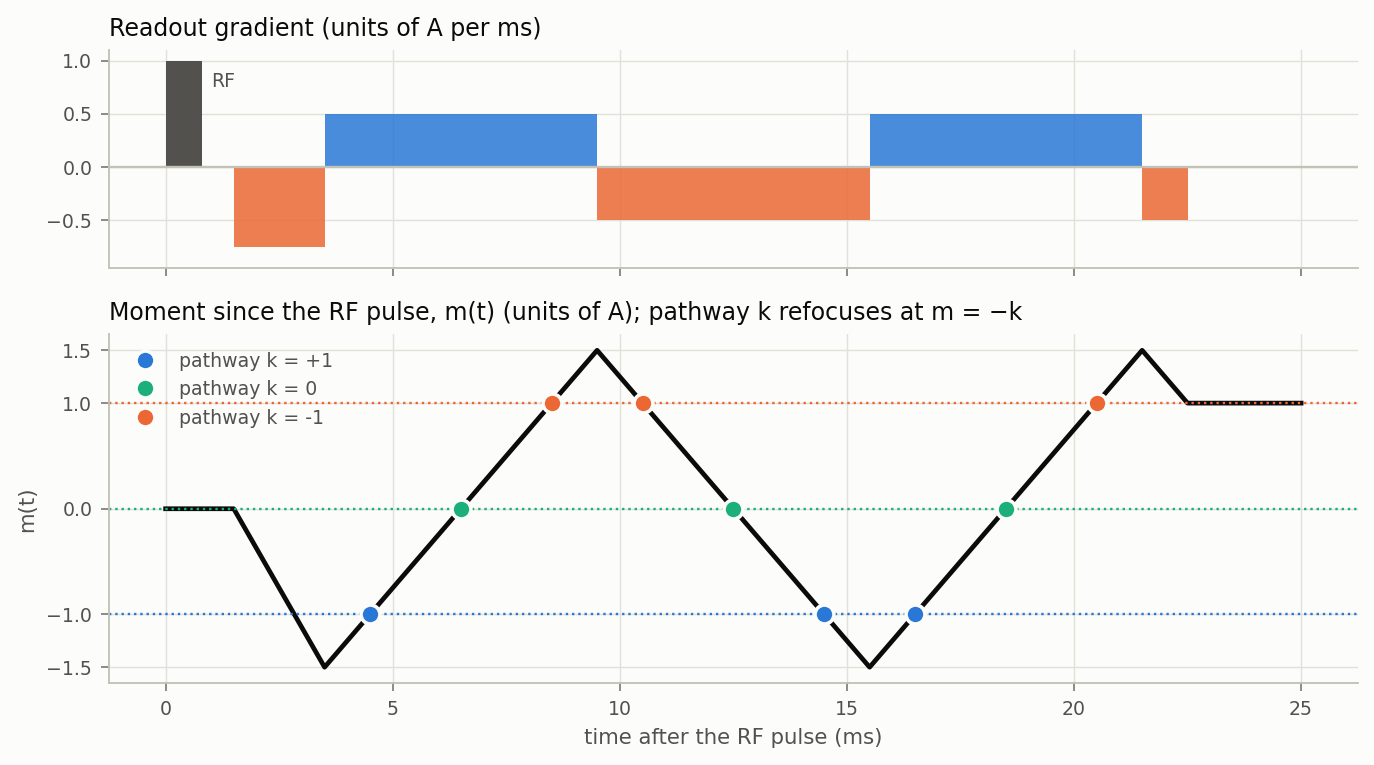
\includegraphics[width=\linewidth]{sequence_timing.png}
\caption{One repetition of the $[+1,0,-1]$ scheme. Top: readout gradient (prephaser, three
readout windows of alternating polarity, rewinder); net area $A$ per repetition. Bottom: the
moment accumulated since the RF pulse; pathway $k$ is refocused (circles) whenever $m(t)=-k$.
The time from the pulse to the first echo (4.5\,ms) is an assumption; the paper does not
state it.}
\label{fig:sequence}
\end{figure}

\begin{table}[!htbp]
\centering
\caption{Published in-vivo protocol~\cite{cheng2019} and the values used in this note.}
\label{tab:protocol}
\small
\begin{tabular}{ll}
\toprule
Repetition time & $\TR=25$\,ms (both scans)\\
Nominal flip angles & $\alpha_1^{\rm nom}=15^\circ$, $\alpha_2^{\rm nom}=330^\circ$ (hard pulses)\\
Pathways & $k\in\{+1,0,-1\}$; three readout windows\\
Pathway spacing & $2.0$\,ms in vivo ($1.86$\,ms phantom); 501\,Hz/pixel\\
Echo times (ms) & $k=+1$: $4.5,14.5,16.5$;\ $k=0$: $6.5,12.5,18.5$;\ $k=-1$: $8.5,10.5,20.5$\\
Scan 2 coverage & central $25\%\times25\%$ of $k_y$--$k_z$\\
Resolution, matrix & $1.2\times1.0\times1.2$\,mm$^3$, $160\times192\times160$, 11.5\,min\\
\bottomrule
\end{tabular}
\end{table}

\subsection{Configuration states}

Let $\psi\in[0,2\pi)$ be the intravoxel phase imparted by one repetition of the unbalanced
gradient and expand
\begin{equation}
  M^+(\psi)=\sum_kF_k\,\E^{ik\psi},\qquad M_z(\psi)=\sum_kZ_k\,\E^{ik\psi},\qquad
  Z_{-k}=\overline{Z_k}.
\end{equation}
One repetition consists of~\cite{hennig1991,weigel2015}:
\begin{align}
  \text{RF:}\quad F_k'&=\cos^2\tfrac{\alpha}{2}F_k+\E^{2i\varphi}\sin^2\tfrac{\alpha}{2}\overline{F_{-k}}
     -i\E^{i\varphi}\sin\alpha\,Z_k,\nonumber\\
  Z_k'&=-\tfrac{i}{2}\E^{-i\varphi}\sin\alpha\,F_k+\tfrac{i}{2}\E^{i\varphi}\sin\alpha\,\overline{F_{-k}}
     +\cos\alpha\,Z_k,\\
  \text{relaxation:}\quad F_k&\to E_2F_k,\quad Z_k\to E_1Z_k\ (k\ne0),\quad
     Z_0\to E_1Z_0+\Mzero(1-E_1),\nonumber\\
  \text{gradient:}\quad F_k&\to F_{k+1}.\nonumber
\end{align}
We write $a_k(\alpha,\Tone,\Ttwo,\dw)$ for the steady-state amplitude of $F_k$ immediately
after the pulse, per unit $\Mzero$.

\subsection{Exact steady state}

The steady state can be computed without truncating the configuration space. An isochromat
whose total precession per repetition is $\beta=\psi+\dw\TR$ has the post-pulse steady state
\begin{equation}
  \bigl(I-R\,R_z(\beta)\,\mathrm{diag}(E_2,E_2,E_1)\bigr)\,\mathbf M^+=(1-E_1)\,R\,\hat{\mathbf z},
  \qquad R=R_z(\varphi)R_x(\alpha)R_z(-\varphi),
  \label{eq:iso}
\end{equation}
and $a_k$ is the $k$-th Fourier coefficient of $M^+(\psi)=M_x^++iM_y^+$ over $\psi$. On a uniform
grid of $n$ isochromats this is a discrete Fourier transform; orders with $|k|<n/2$ are exact
up to aliasing of orders differing by $n$, which decay as $E_2^{n}$-like factors. For every
tissue in this note, including CSF ($\Ttwo=1.5$\,s) at $330^\circ$, $n=128$ reproduces
$n=16\,384$ to $10^{-15}$.

\begin{proposition}[Off-resonance only adds phase]\label{prop:offres}
In the fully dephased regime
\[
  a_k(\dw)=a_k(0)\,\E^{ik\dw\TR};
\]
in particular $|a_k|$ does not depend on $\dw$.
\end{proposition}
\begin{proof}
By \eqref{eq:iso} the steady state depends on $\psi$ and $\dw$ only through $\beta=\psi+\dw\TR$,
so $M^+_{\dw}(\psi)=M^+_0(\psi+\dw\TR)$. Shifting a $2\pi$-periodic function by $\theta$ multiplies
its $k$-th Fourier coefficient by $\E^{ik\theta}$.
\end{proof}

\subsection{Two invariants per scan}

\begin{theorem}[Exact two-invariant reduction]\label{thm:uv}
Let $\varphi=0$ and, for one scan with flip angle $\alpha$, define
\begin{equation}
  u=\frac{E_1-\cos\alpha}{1-E_1\cos\alpha},\qquad
  v=\frac{\sin\alpha\,(1-E_1)}{1-E_1\cos\alpha}.
  \label{eq:uv}
\end{equation}
Then for every pathway $k$ and every $\dw$
\begin{equation}
  a_k(\alpha,\Tone,\Ttwo,\dw)=v\;G_k(u,E_2,\dw),
  \label{eq:uvform}
\end{equation}
where $G_k$ does not depend on $\alpha$ or $\Tone$ otherwise.
\end{theorem}
\begin{proof}
Let $(x,y,z)$ be the pre-pulse state of one isochromat and $w=x+iy$. The pulse $R_x(\alpha)$
maps it to $(x,\ cy-sz,\ sy+cz)$ with $c=\cos\alpha$, $s=\sin\alpha$; relaxation and precession by
$\beta$ then give the next pre-pulse state. The steady state therefore satisfies
\begin{equation}
  w=E_2\E^{i\beta}\bigl(x+i(cy-sz)\bigr),\qquad z=E_1(sy+cz)+1-E_1 .
  \label{eq:steady2}
\end{equation}
The second equation gives $z=(E_1sy+1-E_1)/(1-E_1c)$; note $1-E_1c>0$. Substituting,
\[
  cy-sz=y\,\frac{c-E_1c^2-E_1s^2}{1-E_1c}-\frac{s(1-E_1)}{1-E_1c}=-u\,y-v .
\]
The post-pulse transverse magnetisation is $m_\perp=x+i(cy-sz)=x-iuy-iv$, and $w=E_2\E^{i\beta}m_\perp$.
Eliminating $x=\Re w$ and $y=\Im w$,
\begin{equation}
  m_\perp=\Re\bigl(E_2\E^{i\beta}m_\perp\bigr)-iu\,\Im\bigl(E_2\E^{i\beta}m_\perp\bigr)-iv .
  \label{eq:mperp_lin}
\end{equation}
This is a real-linear equation for $m_\perp$ (two real unknowns) whose coefficients involve only
$u$, $E_2$ and $\beta$, and whose inhomogeneous term is $-iv$. Its $2\times2$ real matrix is
$I-E_2\,D_u\,R(\beta)$ with $D_u=\mathrm{diag}(1,u)$ and $R(\beta)$ a planar rotation; since
$|u|\le1$ and $E_2<1$, $\|E_2D_uR(\beta)\|\le E_2<1$, so it is invertible. Hence
$m_\perp=v\,g(u,E_2,\beta)$ with $g$ independent of $\alpha$ and $\Tone$, and taking Fourier
coefficients over $\psi$ (with $\beta=\psi+\dw\TR$) gives \eqref{eq:uvform}.
\end{proof}

\begin{lemma}\label{lem:absv}
$|u|\le1$ and $|v|=\sqrt{1-u^2}\,\sqrt{\tanh\bigl(\TR/(2\Tone)\bigr)}$.
\end{lemma}
\begin{proof}
From \eqref{eq:uv}, $1-u=(1-E_1)(1+c)/(1-E_1c)$ and $1+u=(1+E_1)(1-c)/(1-E_1c)$, both
non-negative, so $|u|\le1$ and $1-u^2=(1-E_1^2)\,s^2/(1-E_1c)^2$. Hence
$v^2=s^2(1-E_1)^2/(1-E_1c)^2=(1-u^2)(1-E_1)/(1+E_1)$, and $(1-E_1)/(1+E_1)=\tanh(\TR/2\Tone)$ for
$E_1=\E^{-\TR/\Tone}$.
\end{proof}

The invariants take their simplest form in terms of the Ernst angle $\alpha_E=\arccos E_1$, the
flip angle that maximises the spoiled-gradient-echo signal of the tissue.

\begin{proposition}[Ernst-angle form of the invariants]\label{prop:ernst}
Let $\zeta=\tan(\alpha_E/2)$ and, for a flip angle $\alpha$ that is not an odd multiple of $\pi$,
\begin{equation}
  \xi=\frac{\tan(\alpha/2)}{\tan(\alpha_E/2)},\qquad \vartheta=\arctan\xi\in(-\tfrac\pi2,\tfrac\pi2).
  \label{eq:xi}
\end{equation}
Then $\zeta^2=(1-E_1)/(1+E_1)=\tanh(\TR/2\Tone)$ and
\begin{equation}
  u=\frac{\xi^2-1}{\xi^2+1}=-\cos2\vartheta,\qquad
  v=\zeta\,\frac{2\xi}{1+\xi^2}=\zeta\sin2\vartheta .
  \label{eq:ernstform}
\end{equation}
\end{proposition}
\begin{proof}
Write $q=\tan(\alpha/2)$, so $\cos\alpha=(1-q^2)/(1+q^2)$ and $\sin\alpha=2q/(1+q^2)$, and likewise
$E_1=\cos\alpha_E=(1-\zeta^2)/(1+\zeta^2)$, which gives $\zeta^2=(1-E_1)/(1+E_1)=\tanh(\TR/2\Tone)$.
Then $E_1-\cos\alpha=2(q^2-\zeta^2)/D$, $1-E_1\cos\alpha=2(q^2+\zeta^2)/D$ and
$\sin\alpha\,(1-E_1)=4q\zeta^2/D$ with $D=(1+q^2)(1+\zeta^2)$. Substituting in \eqref{eq:uv},
$u=(q^2-\zeta^2)/(q^2+\zeta^2)$ and $v=2q\zeta^2/(q^2+\zeta^2)$; dividing numerator and denominator
by $\zeta^2$ gives \eqref{eq:ernstform}, and $\xi=\tan\vartheta$ gives the trigonometric forms.
\end{proof}

\Cref{lem:absv} is the identity $u^2+(v/\zeta)^2=1$: the pair $(u,v/\zeta)$ lies on the unit
circle at angle $2\vartheta$. $\xi$ measures where the actual flip angle lies relative to the
Ernst angle: $\xi<1$ ($u<0$) below it, $\xi=1$ ($u=0$, $v=\zeta$, the largest value of $v$) at
it, and $\xi\to\infty$ ($u\to1$, $v\to0$) as $\alpha\to\pi$. For $\alpha\ll1$ and $\TR\ll\Tone$,
\begin{equation}
  \xi\approx\frac{\alpha}{\alpha_E}\approx\alpha\sqrt{\frac{\Tone}{2\TR}},\qquad
  \zeta\approx\sqrt{\frac{\TR}{2\Tone}} ,
  \label{eq:xismall}
\end{equation}
so $\xi^2$ is the exact counterpart of the similarity variable $c=\alpha^2\Tone/2\TR$ of
\cref{prop:scaling}. At $15^\circ$ and $\TR=25$\,ms the Ernst angles of WM, GM and CSF are $13.8^\circ$,
$11.0^\circ$ and $6.4^\circ$, so $\xi=1.09$, $1.37$ and $2.36$ ($u=0.08$, $0.30$ and $0.69$). The
small-angle forms are close but not exact: for WM, $\xi^2=1.1787$, $(\alpha/\alpha_E)^2=1.1767$ and
$\alpha^2\Tone/2\TR=1.1652$.

On a logarithmic half-angle axis the invariants take an even simpler form. With
$s=\ln|\tan(\alpha/2)|$ and $s_E=\ln\zeta=\ln\tan(\alpha_E/2)$, so that $|\xi|=\E^{s-s_E}$, \eqref{eq:ernstform} reads
\begin{equation}
  u=\tanh(s-s_E),\qquad |v|=\zeta\,\operatorname{sech}(s-s_E),\qquad \sgn v=\sgn\tan(\alpha/2).
  \label{eq:logtan}
\end{equation}
As a function of $s$, the spoiled-gradient-echo amplitude $|v|$ is a bump of fixed shape
($\operatorname{sech}$), centred at the tissue's Ernst angle $s_E$ and of height $\zeta$. $\Tone$ sets the position and
height of the bump, and the actual flip angle sets the point $s$ at which a scan samples it.
Every log-derivative with respect to $\Bone$ follows from
$\mathrm d\ln|\tan(x/2)|/\mathrm d\ln x=x/\sin x$.

\begin{corollary}[One scan cannot separate $\Mzero$, $\Bone$, $\Tone$]\label{cor:onescan}
For a single scan, with $\Ttwo$, $\Ttwos$, $\dw$, $\phi_0$ fixed, the signal depends on
$(\Mzero,\Bone,\Tone)$ only through the two functions $(u,\ \Mzero v)$. The Jacobian of the
signal with respect to $(\log\Mzero,\log\Bone,\log\Tone)$ has rank at most two, and the
Fisher information about these three parameters is singular at every flip angle.
\end{corollary}
\begin{proof}
By \cref{thm:uv} and the echo factors below (which do not involve $\Mzero$, $\alpha$ or $\Tone$
except through the prefactor $\Mzero$), $S=\Mzero v\,h(u)$ for a function $h$ independent of
$(\Mzero,\Bone,\Tone)$. By the chain rule, the $3$ columns of $\partial S/\partial(\log\Mzero,
\log\Bone,\log\Tone)$ are linear combinations of the $2$ vectors $\partial S/\partial(u,\Mzero v)$,
so they span at most a two-dimensional space. The Fisher information restricted to these
parameters is $J^{\mathsf H}J/\sigma^2$ with $J$ of rank $\le2$, hence singular.
\end{proof}

\subsection{What the invariants mean, and what one scan measures}\label{sec:invariants}

\paragraph{Intuition.} \Cref{fig:logtan} draws \eqref{eq:logtan}. Plot the amplitude $\Mzero|v|$ against
$s=\ln|\tan(\alpha/2)|$: it is a $\operatorname{sech}$ bump of height $\Mzero\zeta$ centred at the Ernst angle, and a scan
samples it at $s=\ln|\tan(\Bone\alpha^{\rm nom}/2)|$. The MPME sequence is not spoiled, but by
\cref{thm:uv} each of its nine signals is $v$ times a function of $u$ alone, so all of them
report the same sample. The ratios between pathways give $u=\tanh(s-s_E)$, the offset of the
sample from the centre of the bump, and the overall scale then gives the height $\Mzero\zeta$.
Neither tells where the sample and the bump lie in absolute terms. Raising $\Bone$ moves the
sample to the right by $\ln[\tan(B_1^{+\prime}\alpha^{\rm nom}/2)/\tan(\Bone\alpha^{\rm nom}/2)]\approx\ln(B_1^{+\prime}/\Bone)$; shortening $\Tone$
by the right amount (about the square of the same factor, since $\zeta\approx\sqrt{\TR/2\Tone}$) moves the
bump by the same distance; and lowering $\Mzero$ by the factor restores the height. The whole
picture translates rigidly, and the scan cannot tell. In words: a larger flip angle in a tissue
with a larger Ernst angle (shorter $\Tone$) is indistinguishable from a smaller flip angle in a
tissue with a smaller Ernst angle.

A second scan samples the same bump at a different $s$. A $330^\circ$ pulse is $-30^\circ$ modulo
$360^\circ$, but its sample moves with $\Bone$ at the rate $\mathrm d\ln|\tan(\alpha_2/2)|/\mathrm d\ln\Bone=\alpha_2/\sin\alpha_2=-11.5$,
against $+1.01$ for the $15^\circ$ pulse. When the family translates the picture to keep scan 1,
the scan-2 sample therefore lands elsewhere on the bump (\cref{fig:logtan}a). A second small
angle such as $30^\circ$ moves at almost the same rate as the first ($1.05$), so its sample
translates with the bump and nearly preserves the data (\cref{fig:logtan}b). This is the
leading-order degeneracy of \cref{prop:scaling} for small-angle protocols.

For small angles, $\xi^2\approx\alpha^2\Tone/2\TR$ is the ratio of the saturation per pulse ($\propto\alpha^2$) to
the recovery per repetition ($\propto\TR/\Tone$), a useful mnemonic for the spoiled part of the signal.
The exact invariant uses half-angle tangents: along the family of \cref{tab:family}, the plain
ratio of the flip angle to the Ernst angle drifts from $1.0851$ to $1.0836$, while $\xi=1.0857$ is
constant.

\begin{figure}[!htbp]
\centering
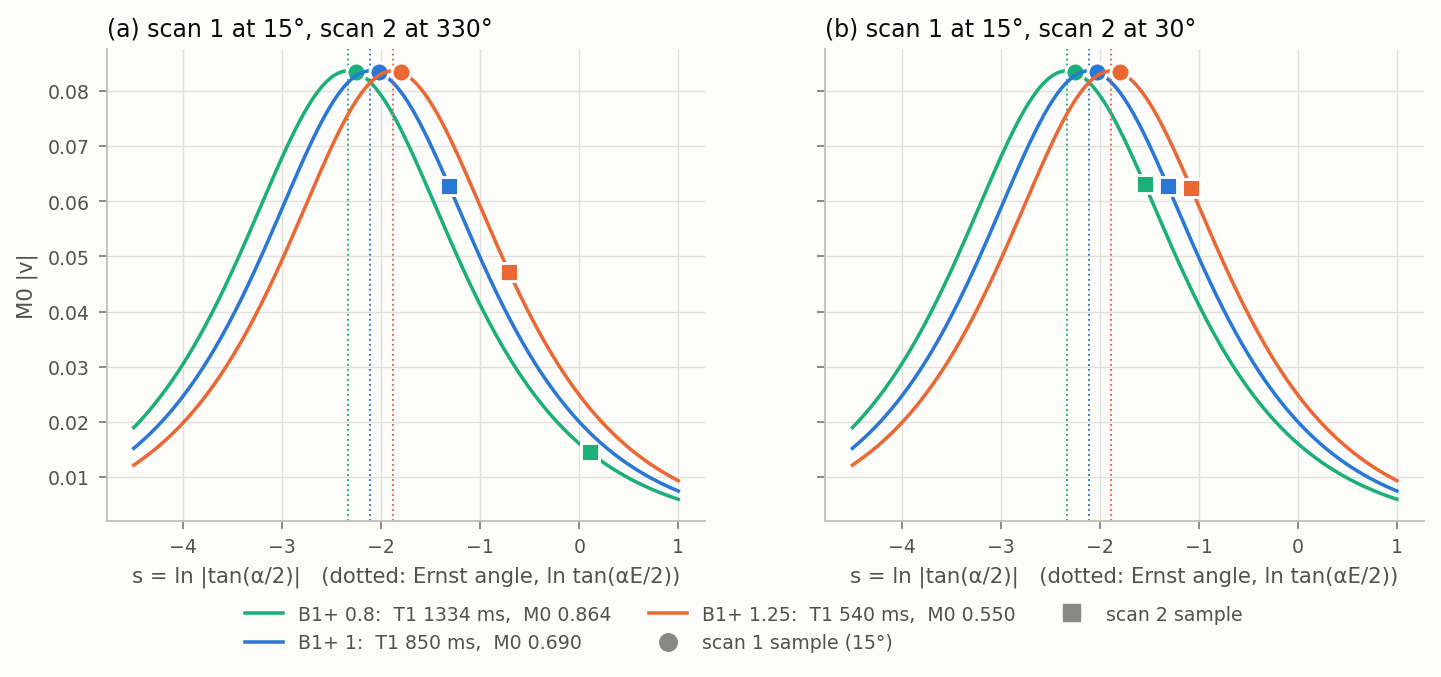
\includegraphics[width=\linewidth]{ernst_logtan.png}
\caption{The single-scan degeneracy on the log half-angle axis (WM, $\TR=25$\,ms). Curves: the
amplitude $\Mzero|v|=\Mzero\zeta\operatorname{sech}(s-s_E)$ for three members of the family \eqref{eq:family}
($B_1^{+\prime}=0.8$, $1$, $1.25$); dotted lines: their Ernst angles $s_E$. Circles: the $15^\circ$ scan-1
sample of each member, at the same offset from its bump and the same height, hence identical
scan-1 data. Squares: the scan-2 sample. (a) For $330^\circ$ the scan-2 samples land at different
heights (and, for $B_1^{+\prime}=1.25$, with the opposite sign of $v$). (b) For $30^\circ$ they almost
coincide: a second small flip angle hardly separates the members.}
\label{fig:logtan}
\end{figure}

\paragraph{Relation to the spoiled gradient echo.} Let $m_z=(1-E_1)/(1-E_1\cos\alpha)$ be the longitudinal
magnetisation (per unit $\Mzero$) just before each pulse in the steady state of a spoiled gradient echo
with the same $\alpha$, $\TR$ and $\Tone$. Then
\begin{equation}
  v=\sin\alpha\;m_z,\qquad u=1-(1+\cos\alpha)\,m_z ,
  \label{eq:uvspoiled}
\end{equation}
since $1-u=(1-E_1)(1+\cos\alpha)/(1-E_1\cos\alpha)$. So $v$ is the spoiled (Ernst) signal: the transverse
magnetisation that each pulse creates from recovered longitudinal magnetisation (the
\emph{source}). $u\in[-1,1]$ is the factor by which one pulse-and-relaxation cycle carries existing
transverse magnetisation into the next repetition (the \emph{retention}, an effective cosine). In
the proof of \cref{thm:uv} they appear as the inhomogeneous term and the coefficient of the
transverse steady-state equation \eqref{eq:mperp_lin}. Unbalanced SSFP differs from the spoiled
sequence only in keeping the transverse magnetisation, and it sees $\alpha$ and $\Tone$ only through
this source and retention.

\paragraph{What one scan measures.} A scan yields 3 pathways $\times$ 3 echoes = 9 complex numbers
(18 real values). By \cref{thm:uv,prop:ernst} and \eqref{eq:signal}, they depend on the
parameters as listed in \cref{tab:onescan}.

\begin{table}[!htbp]
\centering
\caption{Information content of one scan.}
\label{tab:onescan}
\small
\begin{tabular}{ll}
\toprule
Feature of the data & Determined by\\
\midrule
amplitude ratios between pathways, $a_k/a_0=G_k(u)/G_0(u)$ & $u$, i.e.\ $\xi$ (and $E_2$)\\
overall scale, $\Mzero v=\Mzero\zeta\sin2\vartheta$ & $\Mzero\zeta$, given $\xi$\\
decay across the echoes of each pathway & $\Ttwo$ and $\Rtwop$ (hence $\Ttwos$)\\
phase change across echoes & $\dw$\\
common phase & $\phi_0$\\
\bottomrule
\end{tabular}
\end{table}

The 18 values therefore determine six quantities, $(\xi,\,\Mzero\zeta,\,\Ttwo,\,\Rtwop,\,\dw,\,\phi_0)$, and are
redundant with respect to them (which averages noise and allows model checking). The
deficiency is specific: the three unknowns $(\Mzero,\Bone,\Tone)$ enter only through the two
combinations $\xi$ and $\Mzero\zeta$ (equivalently $u$ and $\Mzero v$). More echoes or more pathways
from the same scan do not help, because every one of them depends on $(\alpha,\Tone)$ through the
same pair.

\paragraph{The data model for $(\Mzero,\Bone,\Tone)$.} Write $\xi_i$ and $A$ for the values of $\xi$
and $\Mzero\zeta$ that the data of scan $i$ determine. With $\alpha_i=\Bone\alpha_i^{\rm nom}$, the equations
that $(\Mzero,\Bone,\Tone)$ must satisfy are
\begin{equation}
  \frac{\tan(\Bone\alpha_i^{\rm nom}/2)}{\sqrt{\tanh(\TR/2\Tone)}}=\xi_i,\qquad
  \Mzero\sqrt{\tanh(\TR/2\Tone)}=A ,
  \label{eq:datamodel}
\end{equation}
equivalent to $u(\alpha_i,E_1)=U_i$ and $\Mzero v(\alpha_i,E_1)=V_i$ with $U_i=(\xi_i^2-1)/(\xi_i^2+1)$ and
$V_i=2A\xi_i/(1+\xi_i^2)$. Because all scans share $\TR$, the amplitude equation is the same for every
scan; only $\xi_i$ is new in each. For \emph{one} scan, \eqref{eq:datamodel} is two equations in three
unknowns, and its solutions form a one-parameter family. With the trial transmit scale
$B_1^{+\prime}$ as the parameter, $\tan(\alpha_E'/2)=\tan(B_1^{+\prime}\alpha^{\rm nom}/2)/\xi$, that is,
\begin{equation}
  \Tone'(B_1^{+\prime})=\frac{\TR}{2\,\operatorname{artanh}\bigl(\tan^2(B_1^{+\prime}\alpha^{\rm nom}/2)/\xi^2\bigr)},\qquad
  \Mzero'(B_1^{+\prime})=\Mzero\,\frac{\xi\,\zeta}{\tan(B_1^{+\prime}\alpha^{\rm nom}/2)} .
  \label{eq:family}
\end{equation}
In terms of $E_1$ this is $E_1'=(U+c')/(1+Uc')$ with $c'=\cos(B_1^{+\prime}\alpha^{\rm nom})$, the form used in
\cref{prop:singlescan}. A member exists whenever $|\tan(B_1^{+\prime}\alpha^{\rm nom}/2)|<|\xi|$, equivalently
$c'>-U$ (the Ernst angle must stay below $90^\circ$). Every member reproduces the scan exactly
(\cref{prop:singlescan}). With $x=B_1^{+\prime}\alpha^{\rm nom}$ and $\tau'=\TR/\Tone'$, differentiating \eqref{eq:family} gives
\begin{equation}
  \frac{\mathrm d\ln\Mzero'}{\mathrm d\ln B_1^{+\prime}}=-\frac{x}{\sin x},\qquad
  \frac{\mathrm d\ln\Tone'}{\mathrm d\ln B_1^{+\prime}}=-2\,\frac{x}{\sin x}\,\frac{\sinh\tau'}{\tau'},
  \label{eq:familyslopes}
\end{equation}
the exact forms of the factors $-1$ and $-2$ of \cref{prop:scaling}. For WM at $15^\circ$ they are
$-1.0115$ and $-2.023$, the slope measured in \cref{tab:singlescan}.

\paragraph{What a second flip angle adds.} Dividing the first equation of \eqref{eq:datamodel} for
$i=2$ by that for $i=1$ eliminates $\Tone$ and $\Mzero$:
\begin{equation}
  f(\Bone)\equiv\frac{\tan(\Bone\alpha_2^{\rm nom}/2)}{\tan(\Bone\alpha_1^{\rm nom}/2)}=\frac{\xi_2}{\xi_1}.
  \label{eq:secondscan}
\end{equation}
This is one equation in $\Bone$ alone, the half-angle analogue of the double-angle method. Its roots
are isolated, and $\Tone$ and $\Mzero$ then follow from \eqref{eq:family}. Its sensitivity to $\Bone$ is
the exact lever
\begin{equation}
  L=\frac{\mathrm d\ln|f|}{\mathrm d\ln\Bone}=\frac{\alpha_2}{\sin\alpha_2}-\frac{\alpha_1}{\sin\alpha_1}
  \qquad(\text{actual angles}),
  \label{eq:leverexact}
\end{equation}
$-12.53$ for $15^\circ/330^\circ$ and $+0.036$ for $15^\circ/30^\circ$ at $\Bone=1$ (\cref{sec:information}).

The data fix $\xi_i^2$ through $u_i$. Complex data with a phase $\phi_0$ shared by the two scans also fix
the relative sign of $v_1$ and $v_2$, hence the sign of $\xi_2/\xi_1$; magnitude data fix only
$|\xi_2/\xi_1|$. The aliases of \cref{prop:equiv} are the other roots of $f(B_1^{+\prime})=f(\Bone)$ (complex
data) or $|f(B_1^{+\prime})|=|f(\Bone)|$ (magnitude data). Their $\Bone$ values depend on the true $\Bone$ alone,
not on the tissue; the tissue enters only through the alias $\Tone'$, from \eqref{eq:family}, and
through admissibility ($\zeta'<1$). For the published protocol and true $\Bone=1$ ($f=-2.04$), the
magnitude alias is $B_1^{+\prime}=1.20$ ($f=+2.04$, scan 2 negated); it lies inside the physiological range and
is removed only by the shared phase (the FID-sign test of \cref{sec:magnitude}). The complex alias
is $B_1^{+\prime}=2.01$, which the bound $\Bone\le540/330$ excludes. Within the fitting range
$\Bone\in[\E^{-1},540/330]$, the complex equation has a single root for every true $\Bone$ between $6/11$ and
$1.592$, i.e.\ true $\alpha_2$ between $180^\circ$ and $525^\circ$. Because $f$ is the same function in every
voxel, a $\Bone$ shared by many voxels has the same aliases (\cref{sec:shared}).

\paragraph{A concrete example.} \Cref{tab:family} evaluates \eqref{eq:family} for one
white-matter voxel ($\Tone=850$\,ms, $\Mzero=1$, $\Bone=1$, scan 1 at $15^\circ$, $\TR=25$\,ms; $\xi=1.086$). As $B_1^{+\prime}$
runs from $0.8$ to $1.5$, the flip angle and the Ernst angle move together (their half-angle tangents
keep the ratio $\xi$). $\Tone'$ falls from $1334$ to $372$\,ms and $\Mzero'$ from $1.25$ to $0.66$. Every
member reproduces all nine complex scan-1 signals to machine precision, while the scan-2
($330^\circ$) signals differ by $41\%$ to $200\%$ (of the largest scan-2 signal) for every member except
the truth. The predicted ratio $\xi_2/\xi_1$ for a $330^\circ$ scan changes from $-10.6$ to $+12.1$ across the
family, whereas for a $30^\circ$ scan it changes only from $2.022$ to $2.082$. The second scan fixes
$\Bone$ when its angle moves differently with $\Bone$; more scan-1 data cannot.

\begin{table}[!htbp]
\centering
\caption{The single-scan solution family \eqref{eq:family} for one white-matter voxel (truth:
$\Bone=1$, $\Tone=850$\,ms, $\Mzero=1$). $B_1^{+\prime}\alpha$: actual scan-1 flip angle; $\alpha_E'$: Ernst angle of
$\Tone'$. Misfit: largest difference of the nine complex signals from the true ones, relative to
the largest true signal of that scan. Predicted $\xi_2/\xi_1$: the ratio $f(B_1^{+\prime})$ of
\eqref{eq:secondscan} that the member predicts for a second scan at $330^\circ$ or $30^\circ$; the data
have $f(1)$. Generated by \texttt{scripts/single\_scan\_family.py}.}
\label{tab:family}
\small\setlength{\tabcolsep}{4.5pt}
\begin{tabular}{ccccccccc}
\toprule
& & & & & \multicolumn{2}{c}{misfit} & \multicolumn{2}{c}{predicted $\xi_2/\xi_1$}\\
\cmidrule(lr){6-7}\cmidrule(lr){8-9}
$B_1^{+\prime}$ & $B_1^{+\prime}\alpha$ ($^\circ$) & $\alpha_E'$ ($^\circ$) & $\Tone'$ (ms) & $\Mzero'$ & scan 1 ($15^\circ$) & scan 2 ($330^\circ$) & $330^\circ$ & $30^\circ$\\
\midrule
0.80 & 12.0 & 11.06 & 1334 & 1.253 & $1\times10^{-15}$ & 0.69 & $-10.57$ & $2.022$\\
0.90 & 13.5 & 12.44 & 1052 & 1.112 & $2\times10^{-15}$ & 0.41 & $-5.18$ & $2.028$\\
1.00 & 15.0 & 13.83 & 850 & 1.000 & $2\times10^{-16}$ & 0.00 & $-2.04$ & $2.035$\\
1.10 & 16.5 & 15.21 & 701 & 0.908 & $3\times10^{-16}$ & 1.36 & $+0.18$ & $2.043$\\
1.20 & 18.0 & 16.60 & 587 & 0.831 & $5\times10^{-16}$ & 2.00 & $+2.05$ & $2.051$\\
1.50 & 22.5 & 20.76 & 372 & 0.662 & $1\times10^{-15}$ & 1.27 & $+12.14$ & $2.082$\\

\bottomrule
\end{tabular}
\end{table}

\subsection{Echo evolution and the voxel signal}

Pathway $k$ read at time $t$ after the pulse carries, for one isochromat, the off-resonance
phase $\dw(t+k\TR)$ (\cref{prop:offres} plus precession since the pulse). An intravoxel
frequency distribution with Lorentzian density $\ell(\delta)=(\Rtwop/\pi)/(\Rtwop{}^2+\delta^2)$
averages this to
\begin{equation}
  \int_{-\infty}^{\infty}\ell(\delta)\,\E^{i\delta\tau}\,d\delta=\E^{-\Rtwop|\tau|},
  \label{eq:lorentz}
\end{equation}
the characteristic function of the Cauchy distribution. Together with transverse relaxation
since the pulse, the noise-free signal of scan $i$, echo $j$, pathway $k$ is
\begin{equation}
  \boxed{\;S_{ijk}=\Mzero\,a_k\bigl(\Bone\alpha_i^{\rm nom},\Tone,\Ttwo,0\bigr)\,
  \E^{-t_{ijk}/\Ttwo}\,\E^{-\Rtwop|t_{ijk}+k\TR|}\,
  \E^{i(\phi_0+\dw(t_{ijk}+k\TR))}\;}
  \label{eq:signal}
\end{equation}
For $k\ge0$ the magnitude decays at $1/\Ttwo+\Rtwop=1/\Ttwos$; for $k<0$ and $t<|k|\TR$ at
$1/\Ttwo-\Rtwop$, a spin echo forming at $t=|k|\TR$. Echo times differ between pathways, and
$t+k\TR$ differs in sign between them, which is what separates $\Ttwo$ from $\Rtwop$.

\subsection{Closed forms for $k=0,-1$}

For the two lowest pathways the steady-state magnitudes have the closed forms of unbalanced
FISP and PSIF,
\begin{align}
  |a_0|&=\Bigl|\tan\tfrac{\alpha}{2}\Bigl[1-\frac{(E_1-\cos\alpha)(1-E_2^2)}{r}\Bigr]\Bigr|,\qquad
  |a_{-1}|=\Bigl|\frac{\tan\frac{\alpha}{2}}{E_2}\Bigl[1-\frac{(1-E_1\cos\alpha)(1-E_2^2)}{r}\Bigr]\Bigr|,
  \label{eq:fisp}\\
  r^2&=p^2-q^2,\quad p=1-E_1\cos\alpha-E_2^2(E_1-\cos\alpha),\quad q=E_2(1-E_1)(1+\cos\alpha).
  \nonumber
\end{align}
The PSIF formula in the literature is the echo amplitude at $t=\TR$, hence the factor $1/E_2$.
Dividing $p$ and $q$ by $1-E_1\cos\alpha$ shows that both brackets depend on $(\alpha,E_1)$ only
through $u$, and $\tan(\alpha/2)=v/(1-u)$, in agreement with \cref{thm:uv}.

\subsection{Imaging and noise}

Image formation $y_{ijkc}=\mathcal M_i\mathcal F(C_cS_{ijk})+n_{ijkc}$ (coil maps $C_c$, Fourier
transform $\mathcal F$, sampling $\mathcal M_i$) is linear. Voxel-wise, the coil-combined
complex images are modelled as $S_{ijk}+n_{ijk}$ with independent circular Gaussian noise of
standard deviation $\sigma$ per real and imaginary part; magnitudes are then Rician. The
published low-resolution scan 2 is modelled in \cref{sec:phantom} by truncation of $k$-space.

\subsection{Validation}

\begin{table}[!htbp]
\centering
\caption{Numerical checks of the forward model (all are unit tests).}
\label{tab:validation}
\small
\begin{tabular}{p{0.55\linewidth}l}
\toprule
Check & Agreement\\
\midrule
Isochromat solver vs truncated EPG ($K=400$), pathways $-3\ldots2$, four tissues incl.\ CSF & $<10^{-5}$ absolute\\
$|a_0|$, $|a_{-1}|$ vs closed forms \eqref{eq:fisp} & $10^{-6}$ relative\\
\Cref{thm:uv}: $a_k$ at $(\alpha',E_1')$ with equal $u$ equals $(v'/v)\,a_k$, six pathways, incl.\ $330^\circ$, $\dw\ne0$ & $10^{-9}$ relative\\
\Cref{prop:offres}: $a_k(\dw)=a_k(0)\E^{ik\dw\TR}$ & $10^{-10}$ absolute\\
Echo log-slopes $-(1/\Ttwo+\Rtwop)$ ($k\ge0$), $-(1/\Ttwo-\Rtwop)$ ($k=-1$) & exact\\
128 vs 16\,384 isochromats, CSF at $15^\circ$ and $330^\circ$ & $10^{-15}$ relative\\
\bottomrule
\end{tabular}
\end{table}

\section{The published inverse}\label{sec:paper}

Cheng et al.~\cite{cheng2019} map the parameters by a sequence of closed-form steps applied to
magnitude images. We present their sequential version (scan 2 acquired after scan 1), using
their equation numbers, and verify it against the model of \cref{sec:model}.

\begin{figure}[!htbp]
\centering
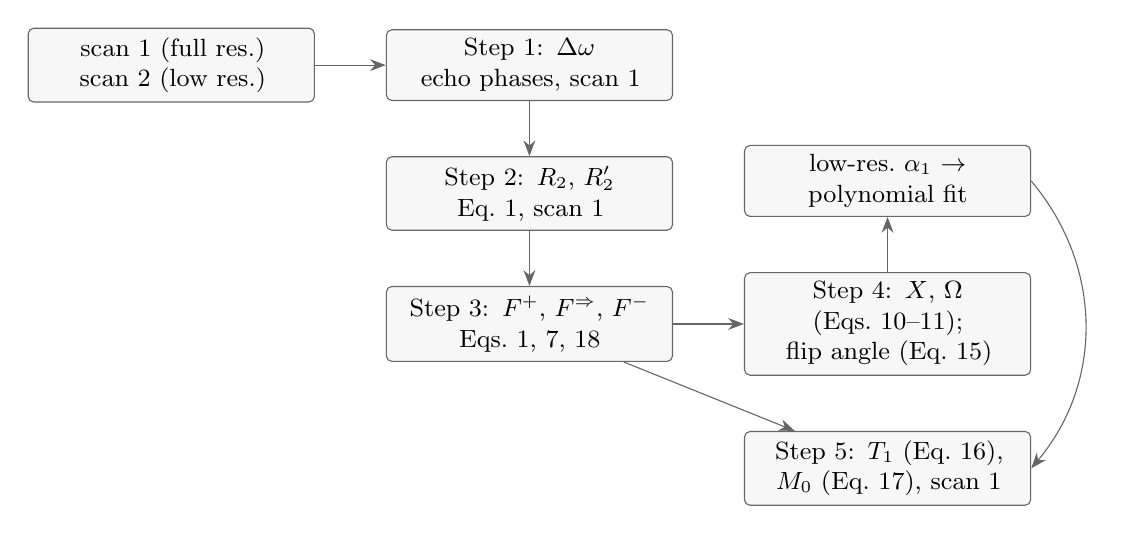
\begin{tikzpicture}[node distance=7mm and 9mm,
  box/.style={draw=black!60, rounded corners=2pt, fill=black!3, align=center, font=\small,
              minimum height=8mm, text width=3.4cm},
  arr/.style={-{Stealth[length=2mm]}, black!60}]
\node[box] (data) {scan 1 (full res.)\\ scan 2 (low res.)};
\node[box, right=of data] (b0) {Step 1: $\dw$\\ echo phases, scan 1};
\node[box, below=of b0] (t2) {Step 2: $R_2$, $\Rtwop$\\ Eq.~1, scan 1};
\node[box, below=of t2] (f) {Step 3: $F^+$, $F^\Rightarrow$, $F^-$\\ Eqs.~1, 7, 18};
\node[box, right=of f] (x) {Step 4: $X$, $\Omega$ (Eqs.~10--11);\\ flip angle (Eq.~15)};
\node[box, above=of x] (b1) {low-res.\ $\alpha_1$ $\rightarrow$\\ polynomial fit};
\node[box, below=of x] (t1) {Step 5: $\Tone$ (Eq.~16),\\ $\Mzero$ (Eq.~17), scan 1};
\draw[arr] (data) -- (b0); \draw[arr] (b0) -- (t2); \draw[arr] (t2) -- (f);
\draw[arr] (f) -- (x); \draw[arr] (x) -- (b1); \draw[arr] (b1.east) to[bend left=40] (t1.east);
\draw[arr] (f) -- (t1);
\end{tikzpicture}
\caption{The published reconstruction~\cite{cheng2019}. The flip angle is computed at the
resolution of scan 2 and smoothed by a polynomial; $\Tone$ and $\Mzero$ are then computed
voxel-wise from scan 1.}
\label{fig:flow}
\end{figure}

\subsection{Steps}

\begin{enumerate}
\item \textbf{Off-resonance.} $\dw$ from the phase evolution between echoes, all pathways
  jointly, scan 1.
\item \textbf{Transverse decay.} Their Eq.~1,
  $S_{i,j,k}=F^+_{i,k}\E^{-(R_2\pm\Rtwop)\mathrm{TE}_{i,j,k}}$ with $+$ for $k\ge0$ and $-$ for
  $k<0$, fitted log-linearly to scan 1 with weights $|S|$.
\item \textbf{Real-valued states.} $F^+_{i,k}$ (Eq.~1 at $\mathrm{TE}=0$) and $F^\Rightarrow_{i,k}$
  (at $\mathrm{TE}=\TR$), signed by their Eq.~18 ($+|F|$ for $k\ge0$, $-|F|$ for $k<0$).
  States before the next pulse follow from the gradient shift, $F^-_k=F^\Rightarrow_{k-1}$, and
  the missing one from their Eq.~7, $F^+_k-F^+_{-k}-F^-_k+F^-_{-k}=0$.
\item \textbf{Flip angle.} The scaling factor $\Omega_{i,k}=F^-_{i,k}+F^-_{i,-k}$ (Eq.~10) and
  the \emph{mixing factor} $X_{i,k}=1-2(F^-_{i,k}-F^+_{i,k})/\Omega_{i,k}$ (Eq.~11), with $k=+1$
  for the $[+1,0,-1]$ scheme or $k=-1$ for $[0,-1,-2]$, then Eq.~15,
  \begin{equation}
    \Bigl(\frac{X_1c_1-1}{X_1-c_1}\Bigr)^{T_{R,2}/T_{R,1}}=\frac{X_2c_2-1}{X_2-c_2},\qquad
    c_i=\cos\alpha_i,\quad \alpha_2=\beta\,\frac{\alpha_2^{\rm nom}}{\alpha_1^{\rm nom}}\,\alpha_1,
    \label{eq:p15}
  \end{equation}
  solved for $\alpha_1$, with $\beta=1$ in phantoms and $\beta=1.24$ in vivo (their Eq.~19).
  The branch $\alpha_2<360^\circ$ or $>360^\circ$ is chosen from the relative phase of $F^+_0$ in
  the two scans; $\alpha_2^{\rm nom}\Bone\in[180^\circ,540^\circ]$ is assumed.
\item \textbf{$\Tone$ and $\Mzero$.} Their Eq.~16, read as
  \begin{equation}
    \Tone=\TR\Big/\ln\frac{X_1c_1-1}{X_1-c_1},
    \label{eq:p16}
  \end{equation}
  and Eq.~17 for $\Mzero$, both from scan 1.
\end{enumerate}

\Cref{eq:p16} follows from their own derivation ($Z^+/Z^\Rightarrow=\E^{\TR/\Tone}$); the
extracted text of the author manuscript prints $\TR\ln(\cdot)$, which does not reproduce
$\Tone$. Their Eq.~8, a nutation function $\nu(\alpha,\Delta f)$ that corrects $\cos\alpha$ for
off-resonance during a finite hard pulse, is not used here because our pulses are
instantaneous.

\subsection{Consistency with the forward model}

The intercepts of Eq.~1 are not the configuration amplitudes $a_k$ of \cref{sec:model}: by
\eqref{eq:signal} the magnitude at $\mathrm{TE}=0$ is $\Mzero|a_k|\E^{-\Rtwop|k|\TR}$. The next
proposition shows that this does not matter.

\begin{proposition}[The published relations hold for the forward model]\label{prop:paperconsistent}
Define $\tilde F_k=F_k\,\E^{-\Rtwop|k|\TR}$ for transverse and $\tilde Z_k=Z_k\,\E^{-\Rtwop|k|\TR}$
for longitudinal states. (i) The quantities that Eq.~1 provides are $\tilde F^+_k$ and
$\tilde F^\Rightarrow_k$. (ii) Every relation used in Steps 3--5 (Eqs.~2--7 and 10--17)
holds for the tilde states whenever it holds for the configuration states. Consequently the
published inverse recovers the exact parameters from noise-free data of \eqref{eq:signal}.
\end{proposition}
\begin{proof}
(i) At $\mathrm{TE}=0$, \eqref{eq:signal} gives magnitude $\Mzero|a_k|\E^{-\Rtwop|k|\TR}$,
i.e.\ $|\tilde F^+_k|$; extrapolating the same fit to $\mathrm{TE}=\TR$ gives
$\Mzero|a_k|\E^{-\TR/\Ttwo}\E^{-\Rtwop(|k|\TR\pm\TR)}$ with $+$ for $k\ge0$ and $-$ for $k<0$, which
is $|\tilde F_{k+1}^-|$ because the state of order $k$ after a repetition becomes order $k+1$
and $|k|\pm1=|k+1|$ for those signs. (ii) Each relation in Eqs.~2--7 and 10--17 is linear in
states of a single order $|k|$ (Eq.~2 and the steady-state conditions relate $Z_k$ before and
after a repetition at the same order; Eqs.~4--7 relate $F_{\pm k}$ and $Z_{\pm k}$ across one
pulse; Eqs.~10--11 combine $F_{\pm k}$), or is a ratio of such quantities. Multiplying all
states of order $\pm k$ by the common factor $\E^{-\Rtwop|k|\TR}$ preserves linear relations among
them and leaves ratios unchanged; in particular $X_{i,k}$ is unchanged. Eq.~17 uses $k=0$,
where the factor is $1$. The equations are exact identities of the noise-free steady state,
so the inverse returns the true parameters.
\end{proof}

Numerically, Eqs.~7, 16 and 17 hold to $10^{-12}$ on the steady states of \eqref{eq:iso} for
$\alpha=15^\circ$ and $330^\circ$ and three tissues including CSF, for both $k=\pm1$. That real-valued
states suffice is a consequence of \cref{lem:imag} (\cref{app:proofs}): all configuration
amplitudes are purely imaginary, i.e.\ share the phase $\pm\pi/2$. The specific sign pattern of
Eq.~18 (all $k\ge0$ states with one sign, all $k<0$ with the other) is observed for every
parameter set we examined.

\subsection{Implementation and behaviour}

We implemented Steps 1--5 equation by equation (\texttt{paper.py}). The flip angle is found
by a dense grid over the admissible branch interval followed by bisection on the sign change
of \eqref{eq:p15}. On noise-free data the implementation recovers all parameters to relative
error $10^{-11}$, for both pathway schemes, for $\Bone\in[0.7,1.4]$ (so that $\alpha_2$ crosses
$360^\circ$) and $|\Delta f|\le100$\,Hz.

Two properties matter under noise. First, \eqref{eq:p16} requires $(X_1c_1-1)/(X_1-c_1)>1$;
noise can violate it, and $\Tone$ is then undefined. Second, the inverse is sequential: $R_2$
and $\Rtwop$ are fixed from scan 1 before the flip angle is estimated, and every later step
combines extrapolated, differenced and ratioed estimates whose noise is not controlled. Both
effects are quantified in \cref{sec:ml,sec:phantom}.

\section{What the data determine}\label{sec:information}

\subsection{Fisher information and the Cram\'er--Rao bound}

For complex data with independent Gaussian noise of variance $\sigma^2$ per component,
\begin{equation}
  \Fi(\theta)=\frac{1}{\sigma^2}\sum_{i,j,k}\Re\Bigl[\overline{\partial_\theta S_{ijk}}\;
  \partial_\theta S_{ijk}^{\mathsf T}\Bigr],\qquad
  \operatorname{Cov}(\hat\theta)\succeq\Fi^{-1}
  \label{eq:fisher}
\end{equation}
for every estimator that is (locally) unbiased at $\theta$. Biased estimators---constrained,
regularised or learned ones---are not covered; they can have smaller variance and mean
squared error, at the price of a bias that the CRLB does not quantify (Bayesian bounds such
as the van Trees inequality address that case). With $\sigma$ in units of $\Mzero$ every bound
scales as $\sigma/\Mzero$; we report bounds per unit $\sigma/\Mzero$. Jacobians are computed exactly
(\cref{sec:jacobian}) and agree with automatic differentiation and finite differences.

Three diagnostics describe conditioning: the condition number and smallest eigenpair
$(\lambda,u)$ of the normalised information $\tilde\Fi=D^{-1/2}\Fi D^{-1/2}$, $D=\mathrm{diag}\,\Fi$,
where the direction in original coordinates is $w\propto D^{-1/2}u$ (the generalised eigenvector
of $\Fi w=\lambda Dw$); the variance inflation factors $(\Fi^{-1})_{ll}\Fi_{ll}$; and the
fixed-parameter bias $\delta\theta_r=-\Fi_{rr}^{-1}\Fi_{rm}\delta$ that results from holding
$\theta_m$ at a wrong value.

\subsection{Logarithmic parameters}\label{sec:logparam}

$\Mzero,\Bone,\Tone,\Ttwo,\Ttwos$ are positive scale parameters, and the model depends on them
through dimensionless combinations: by \cref{thm:uv,lem:absv} and \eqref{eq:signal},
$S/\Mzero$ is a function of $\Bone\alpha^{\rm nom}$, $\TR/\Tone$, $\TR/\Ttwo$, $t/\Ttwo$, $\Rtwop t$ and
$\dw\,t$. In log coordinates a change of units is a translation, derivatives are
dimensionless elasticities, and the central symmetry of \cref{prop:scaling} is a straight
line with constant direction $(-1,+1,-2)$ in $(\log\Mzero,\log\Bone,\log\Tone)$; in linear
coordinates its orbits are curves with a direction that varies from voxel to voxel. With
$D_\theta=\mathrm{diag}(\Mzero,\Bone,\Tone,\Ttwo,\Ttwos,1,1)$, $\Fi_{\rm lin}=D_\theta^{-1}\Fi
D_\theta^{-1}$, so $\sqrt{(\Fi^{-1})_{ll}}$ is the local coefficient of variation; for large
spreads it is not ($\mathrm{CV}=\sqrt{\E^{s^2}-1}$ for a Gaussian log-error of SD $s$).
For the relaxation times the likelihood is closer to quadratic in log coordinates (cost
asymmetry for $\pm20\%$ steps: $\Tone$ $0.58$ linear vs $0.87$ log; $\Ttwo$ $0.78$ vs $1.16$),
whereas the signal is exactly linear in $\Mzero$, so for $\Mzero$ the argument for logs is the
symmetry and relative errors, not curvature. Correlations, normalised eigenvalues and
variance inflation factors are identical in both coordinates (the change of variables has a
diagonal Jacobian), so no conclusion below depends on this choice. Positivity is automatic
in log coordinates, but the ordering $\Ttwos\le\Ttwo$ ($\Rtwop\ge0$) is not and must be enforced
by an estimator. $\dw$ and $\phi_0$ are not scale parameters and stay linear; $\log\Ttwos$ is
used rather than $\log\Rtwop$ because $\Rtwop$ may be close to zero.

\subsection{One scan, and small flip angles}

\Cref{cor:onescan} already shows that one scan cannot separate $\Mzero$, $\Bone$ and $\Tone$;
numerically, the scan-1-only bound on $\log\Tone$ with $\Bone$ unknown is $2.4\times10^8$ per unit
$\sigma/\Mzero$. Two scans tied by a common $\Bone$ can, unless both flip angles are small.

\begin{proposition}[Small-angle scaling invariance]\label{prop:scaling}
Fix $\TR$, $\Ttwo$ ($E_2<1$), a pathway $k$ and $\kappa>0$. Let $\alpha\to0$ and $\rho=\TR/\Tone\to0$
with $c=\alpha^2/(2\rho)$ fixed. Then
\begin{equation}
  a_k(\alpha,\Tone)=\alpha\,f_k(c,E_2)+O(\alpha^3+\alpha\rho),\qquad
  \Mzero a_k(\alpha,\Tone)-\tfrac{\Mzero}{\kappa}\,a_k(\kappa\alpha,\Tone/\kappa^2)=O(\alpha^3+\alpha\rho),
  \label{eq:scaling}
\end{equation}
with $f_k(c,E_2)=G_k\bigl(\tfrac{c-1}{c+1},E_2,0\bigr)/(1+c)$. Hence, through \eqref{eq:b1}, the
signal of every scan with a small flip angle is invariant to leading order under
\begin{equation}
  (\Mzero,\ \Bone,\ \Tone)\longmapsto(\Mzero/\kappa,\ \kappa\Bone,\ \Tone/\kappa^2).
  \label{eq:sym}
\end{equation}
The remainder is additive and not uniform in $\kappa$; $\kappa$ is fixed as the limit is taken.
\end{proposition}
\begin{proof}
With $E_1=1-\rho+O(\rho^2)$ and $\cos\alpha=1-\alpha^2/2+O(\alpha^4)$,
\begin{align*}
  u&=\frac{\alpha^2/2-\rho+O(\alpha^4+\rho^2)}{\alpha^2/2+\rho+O(\alpha^4+\rho^2+\alpha^2\rho)}
   =\frac{c-1}{c+1}+O(\alpha^2+\rho),\\
  v&=\frac{\alpha\rho+O(\alpha^3\rho+\alpha\rho^2)}{\rho+\alpha^2/2+O(\alpha^4+\rho^2+\alpha^2\rho)}
   =\frac{\alpha}{1+c}\bigl(1+O(\alpha^2+\rho)\bigr).
\end{align*}
$G_k(u,E_2,0)$ is a Fourier coefficient of the solution of \eqref{eq:mperp_lin}, whose matrix
$I-E_2D_uR(\beta)$ is invertible with inverse bounded by $1/(1-E_2)$ uniformly in $|u|\le1$ and
$\beta$, and depends smoothly on $u$; hence $G_k$ is Lipschitz in $u$ and
$G_k(u)=G_k(\tfrac{c-1}{c+1})+O(\alpha^2+\rho)$. By \cref{thm:uv},
$a_k=v\,G_k(u)=\alpha f_k(c,E_2)+O(\alpha^3+\alpha\rho)$. Under $\alpha\to\kappa\alpha$,
$\rho\to\kappa^2\rho$, $c$ is unchanged and the leading term scales by $\kappa$, which
$\Mzero\to\Mzero/\kappa$ compensates; the remainders are of the stated order for fixed $\kappa$.
Since $\Bone$ multiplies every flip angle, $\alpha\to\kappa\alpha$ is $\Bone\to\kappa\Bone$, and the echo
factors of \eqref{eq:signal} do not involve $\alpha$ or $\Tone$.
\end{proof}

A direct expansion of the isochromat solution gives the same leading term in explicit form,
$m_\perp(\psi)\simeq-i\alpha/\{(1-E_2\E^{i\psi})[1+cH(\psi)]\}$ with
$H=(1-E_2^2)/|1-E_2\E^{i\psi}|^2$ (\cref{app:scaling}). Numerically, with $c=0.75$, the
leading-order formula matches the exact solver for pathways $-3\ldots2$ to $2.5\times10^{-3}$,
$6.2\times10^{-4}$, $1.5\times10^{-4}$, $3.8\times10^{-5}$ (relative to $|a_0|$) at
$\alpha=15^\circ,7.5^\circ,3.75^\circ,1.875^\circ$: the factor four per halving of an $O(\alpha^2)$
relative remainder.

\begin{corollary}[Leading-order degeneracy]\label{cor:degenerate}
If all flip angles are small, the directional derivative of the signal along
$v=(-1,+1,-2,0,0,0,0)$ vanishes at leading order (it is $O(\alpha^3+\alpha\rho)$ while the others
are $O(\alpha)$), so $\Fi$ is ill-conditioned. No number of small-angle acquisitions removes this
leading-order degeneracy, because $\Bone$ scales all of them by the same factor.
\end{corollary}

The degeneracy is of leading order only: at finite angles $\Fi$ is nonsingular and the
parameters are identifiable in principle, but separation is very noise-sensitive. For the
reference tissue the condition number of $\tilde\Fi$ is $2.6\times10^4$ for $30^\circ/60^\circ$,
$5.0\times10^5$ for $15^\circ/30^\circ$ and $2.5\times10^7$ for $3.75^\circ/7.5^\circ$. Repeated
acquisitions shrink all bounds as $1/\sqrt N$ but do not improve conditioning. On the full
model with three pathways, holding $\Bone$ wrong by $\varepsilon$ with $15^\circ/30^\circ$ shifts the
fit by $\delta\log\Tone=-2.06\varepsilon$ and $\delta\log\Mzero=-1.02\varepsilon$ (predicted $-2$, $-1$).

\subsection{How the published protocol escapes}

\begin{proposition}[Periodicity]\label{prop:period}
$a_k(-\alpha)=-a_k(\alpha)$ and $a_k(\alpha+2\pi)=a_k(\alpha)$ for all $k$. Hence two protocols whose
actual flip angles agree up to sign and multiples of $2\pi$ in every scan carry identical
Fisher information about every parameter when $\Bone$ is known; in particular
$15^\circ/330^\circ$ and $15^\circ/30^\circ$ at $\Bone=1$.
\end{proposition}
\begin{proof}
$R_x(-\alpha)=R_z(\pi)R_x(\alpha)R_z(-\pi)$, an RF phase of $\pi$. Precession and relaxation commute
with $R_z$, so the steady state for RF phase $\pi$ is $R_z(\pi)$ applied to the steady state for
phase $0$, which multiplies every $F_k$ by $-1$. Periodicity is that of $R_x$. A known,
scan-wide sign changes neither the likelihood's curvature nor $\Fi$; with $\Bone$ known the actual
angles, not the nominal ones, determine the data.
\end{proof}

The equivalence concerns actual angles: $330^\circ\Bone$ and $-30^\circ\Bone$ agree modulo $360^\circ$ only
at $\Bone=1$ in the physiological range (at $\Bone=1.1$: $363^\circ$ vs $33^\circ$, and known-$\Bone$
$\Tone$ bounds $29.6$ vs $29.0$). Near $\Bone=1$ the value of the large pulse lies in the $\Bone$
derivative of its effective angle $\alpha_2^{\rm eff}=330^\circ\Bone-360^\circ$:
\begin{equation}
  \frac{\partial\log|\alpha_2^{\rm eff}|}{\partial\log\Bone}=\frac{330\,\Bone}{330\,\Bone-360},
  \qquad\frac{\partial\log\alpha_1}{\partial\log\Bone}=1,
  \label{eq:lever}
\end{equation}
which is $-11$ at $\Bone=1$, $-2.75$ at $\Bone=0.8$, and diverges as $\alpha_2^{\rm eff}\to360^\circ$.
\Cref{eq:sym} needs all angles to scale alike; under a $\Bone$ change the second moves much
faster and in the opposite direction, and the near-null direction is lifted.

\Cref{eq:lever} is the small-effective-angle form of an exact statement. By \cref{prop:ernst}, a
scan sees its flip angle through $\ln|\tan(\alpha_i/2)|$, whose log-derivative with respect to $\Bone$ is
$\alpha_i/\sin\alpha_i$. After $\Tone$ and $\Mzero$ are profiled out, only the difference of the two scans
remains, the lever $L=\alpha_2/\sin\alpha_2-\alpha_1/\sin\alpha_1$ of \eqref{eq:leverexact}: at $\Bone=1$ the scan-2
term is $-11.52$ (\cref{eq:lever} gives $-11$), the scan-1 term $1.01$, and $L=-12.53$; for
$15^\circ/30^\circ$, $L=0.036$. At $\Bone=1$ the two protocols produce the same data up to the sign of
scan 2 (\cref{prop:period}), so they differ only in $L$, and the ratio of their $\Bone$ bounds is
$|L_{330}/L_{30}|=351.17$. The computed bounds for WM, $774.40$ and $2.2052$, have exactly this ratio.

\subsection{Bounds and conditioning}

\begin{table}[!htbp]
\centering
\caption{CRLB per unit $\sigma/\Mzero$ (log-parameter SD; rad/ms for $\dw$), both scans at full
resolution.}
\label{tab:crlb}
\small
\begin{tabular}{llcccccc}
\toprule
Protocol & Tissue ($\Tone/\Ttwo/\Ttwos$) & $\Mzero$ & $\Bone$ & $\Tone$ & $\Ttwo$ & $\Ttwos$ & $\dw$\\
\midrule
$15^\circ/330^\circ$ & WM ($850/66/50$) & 12.5 & 2.21 & 27.3 & 16.0 & 27.2 & 0.30\\
$15^\circ/330^\circ$ & GM ($1350/90/60$) & 14.7 & 2.75 & 33.1 & 20.7 & 38.2 & 0.31\\
$15^\circ/330^\circ$ & reference ($1500/70/60$) & 19.0 & 2.91 & 40.5 & 23.1 & 47.3 & 0.37\\
$15^\circ/330^\circ$ & reference, $\Bone$ known & 16.1 & -- & 28.0 & 20.7 & 44.2 & 0.37\\
$15^\circ/30^\circ$ & reference & 1050 & 1020 & 2110 & 23.1 & 47.3 & 0.37\\
$15^\circ/30^\circ$ & reference, $\Bone$ known & 16.1 & -- & 28.0 & 20.7 & 44.2 & 0.37\\
\bottomrule
\end{tabular}
\end{table}

\begin{table}[!htbp]
\centering
\caption{Conditioning (reference tissue).}
\label{tab:cond}
\small
\begin{tabular}{p{0.42\linewidth}p{0.22\linewidth}p{0.26\linewidth}}
\toprule
 & $15^\circ/330^\circ$ & $15^\circ/30^\circ$\\
\midrule
Eigenvalues of $\tilde\Fi$ & $0.024,0.11,0.22,0.51,$ $0.52,1.49,4.13$ & $7.7{\times}10^{-6},0.11,0.29,$ $0.51,0.76,1.49,3.84$\\
Condition number & 173 & $5.0\times10^5$\\
Variance inflation $\Mzero/\Bone/\Tone$ & $16.7/4.6/26.6$ & $51\,000/7\,700/72\,000$\\
Correlations $(\Bone,\Tone)$, $(\Bone,\Mzero)$, $(\Tone,\Mzero)$ & $0.72,0.53,0.77$ & $-0.9999,-0.9999,$ $0.9999$\\
$\partial\log\Tone/\partial\log\Bone$, $\Bone$ fixed, both scans & $+10.1$ & $-2.06$\\
$\partial\log\Tone/\partial\log\Bone$, $\Bone$ fixed, scan 1 only & $-2.02$ & $-2.02$\\
\bottomrule
\end{tabular}
\end{table}

\begin{figure}[!htbp]
\centering
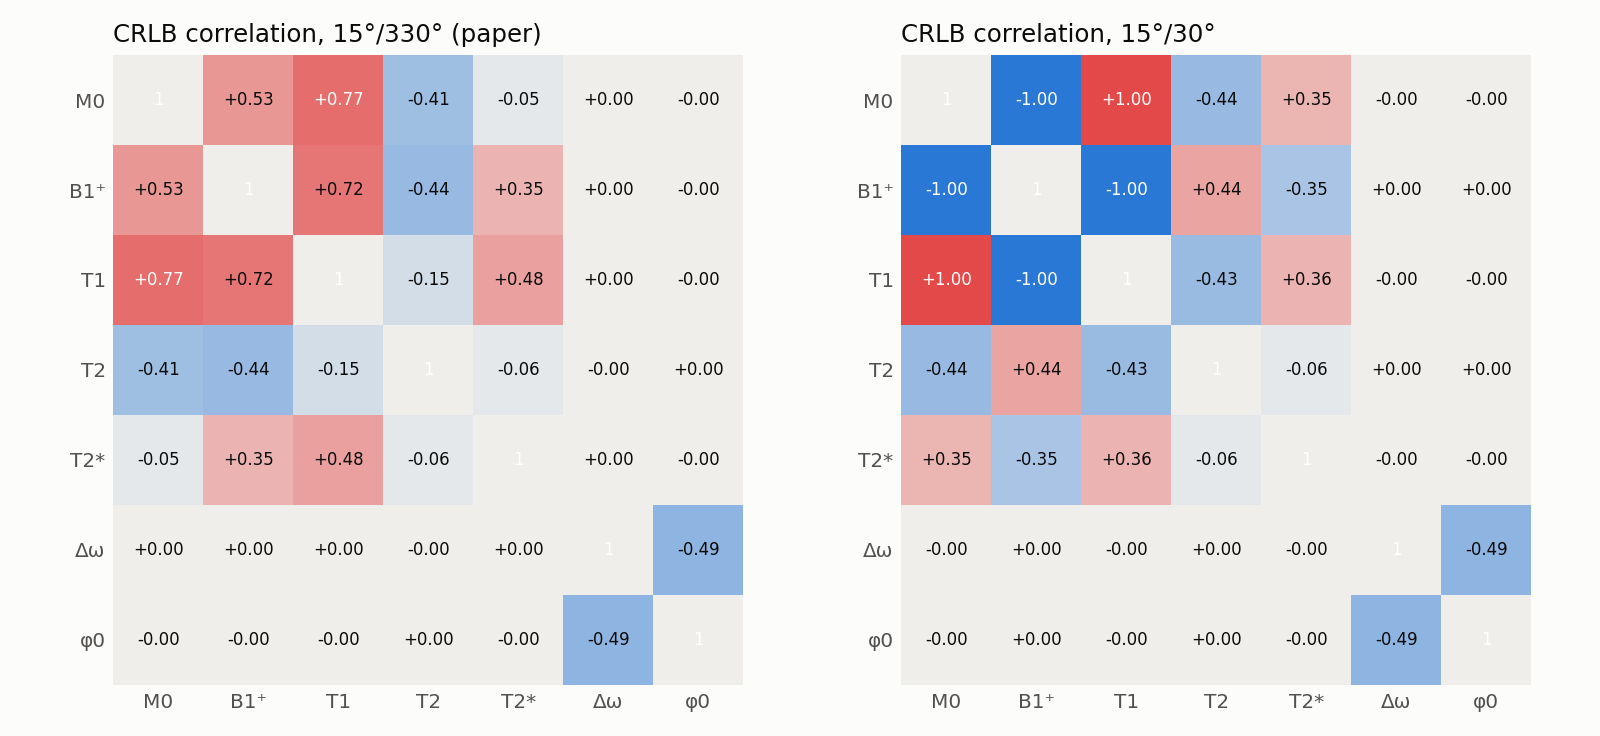
\includegraphics[width=\linewidth]{crlb_correlation.png}
\caption{Correlation matrices of $\Fi^{-1}$. The $\Mzero$--$\Bone$--$\Tone$ block of the small-angle
protocol is perfectly correlated, the signature of \eqref{eq:sym}.}
\label{fig:corr}
\end{figure}

\begin{figure}[!htbp]
\centering
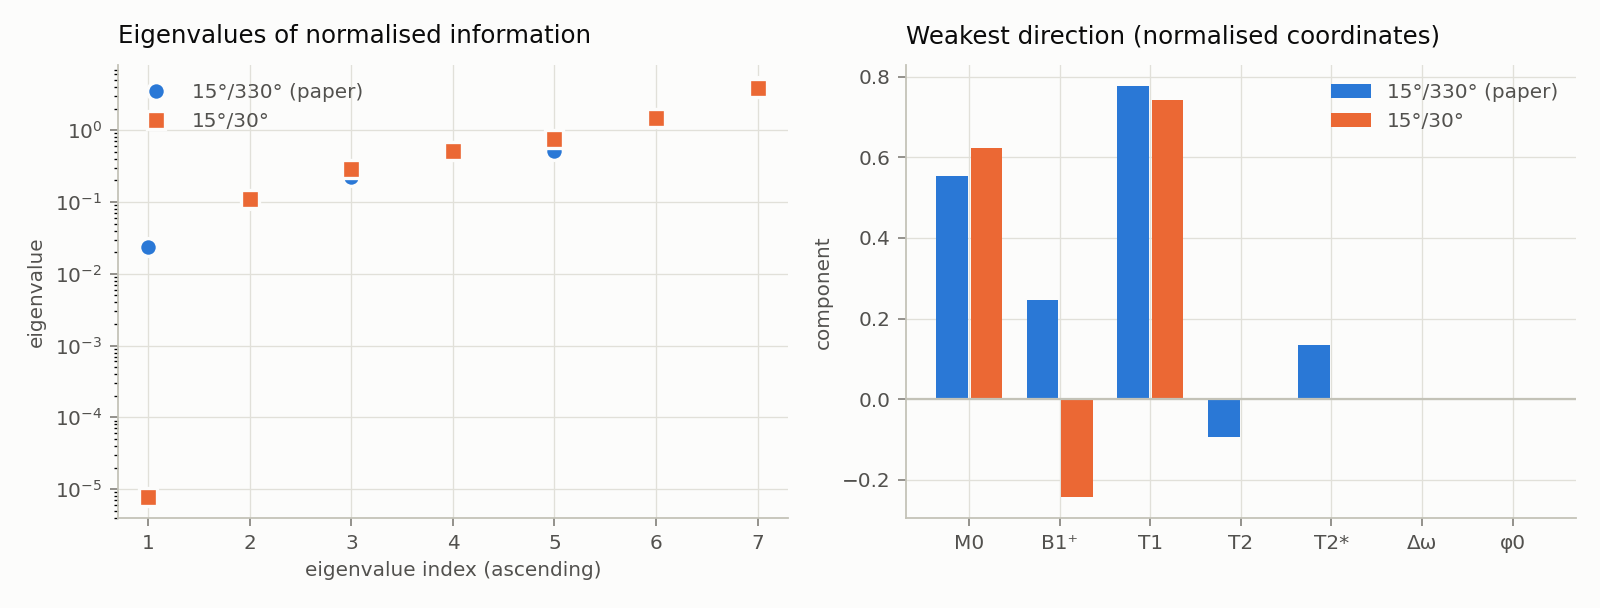
\includegraphics[width=\linewidth]{crlb_eigen.png}
\caption{Left: eigenvalues of $\tilde\Fi$. Right: the weakest direction in log coordinates,
$w\propto D^{-1/2}u$. For $15^\circ/30^\circ$ it is the symmetry direction $(-1,1,-2)/\sqrt6$ (black);
for $15^\circ/330^\circ$ it is dominated by $\Tone$ ($-0.85$), with $\Mzero$ and $\Ttwos$ ($-0.36$ each),
and its $\Bone$ component is only $-0.05$.}
\label{fig:eigen}
\end{figure}

The $\Tone$ bound builds up as groups of parameters are freed: $7.9$ ($\Tone$ only), $21.1$
($+\Ttwo,\Ttwos,\dw,\phi_0$), $28.0$ ($+\Mzero$), $40.5$ ($+\Bone$, $15^\circ/330^\circ$) and $2110$ ($+\Bone$,
$15^\circ/30^\circ$); the factors depend on the order, and the variance inflation factors are the
order-free summary. With the published protocol $\Bone$ is no longer the main source of
$\Tone$ uncertainty: at $15^\circ$ and $\TR=25$\,ms, $\Tone$ is weakly encoded and confounded mostly
with the transverse relaxation times and $\Mzero$. Separating which data are used from whether
$\Bone$ is known gives $\Tone$ bounds of $40.5$ (both scans, $\Bone$ unknown), $28.0$ (both, known),
$57.1$ (scan 1, known) and $2.4\times10^8$ (scan 1, unknown).

\begin{figure}[!htbp]
\centering
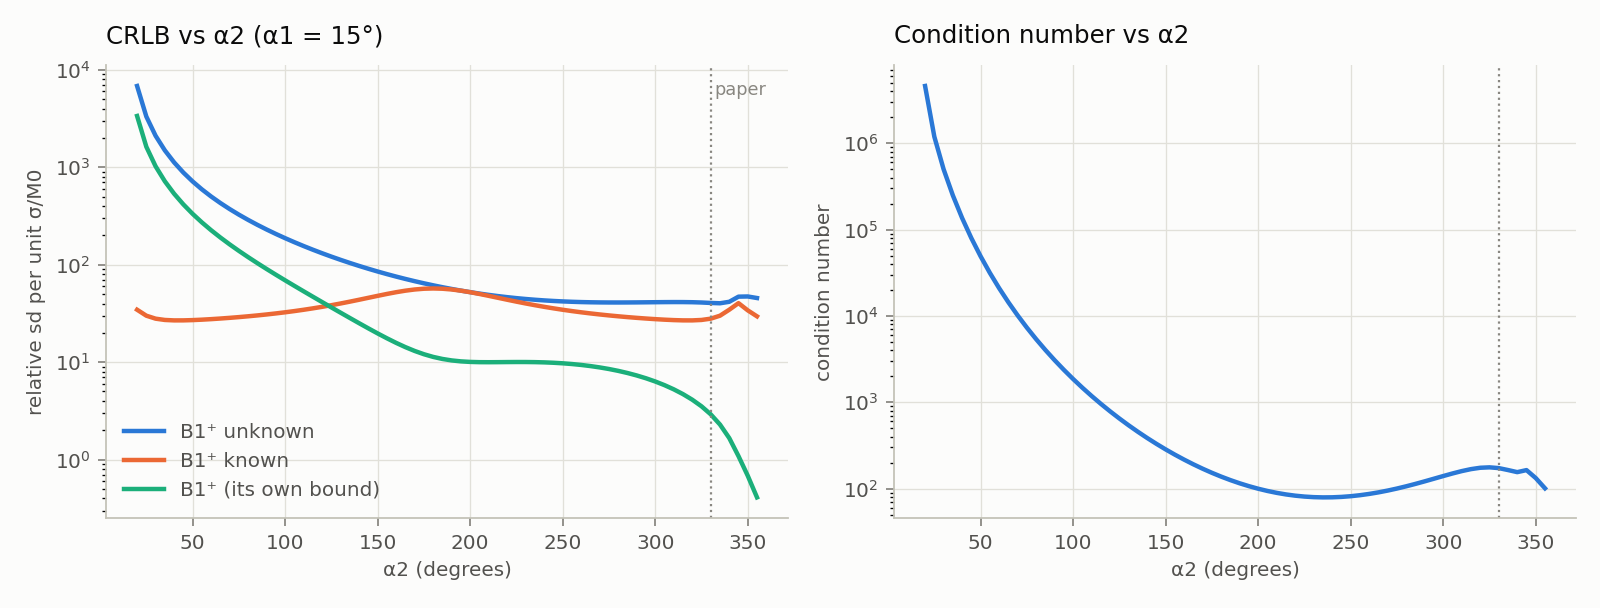
\includegraphics[width=\linewidth]{crlb_flip_sweep.png}
\caption{Bounds and condition number versus $\alpha_2^{\rm nom}$ ($\alpha_1^{\rm nom}=15^\circ$).}
\label{fig:flip}
\end{figure}

\begin{figure}[!htbp]
\centering
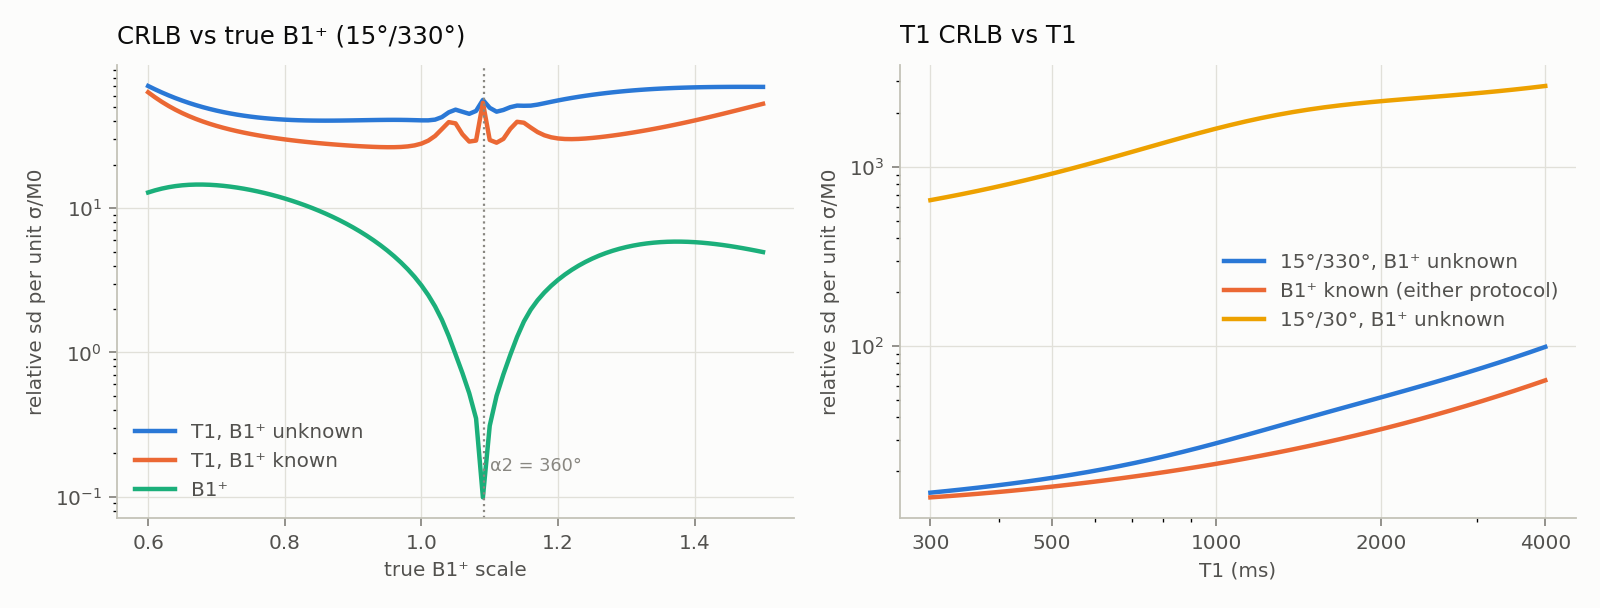
\includegraphics[width=\linewidth]{crlb_b1_t1_sweeps.png}
\caption{Left: bounds versus the true $\Bone$; $\Bone$ is locally best determined where
$\alpha_2^{\rm eff}=360^\circ$. Right: $\Tone$ bound versus $\Tone$.}
\label{fig:sweeps}
\end{figure}

\begin{figure}[!htbp]
\centering
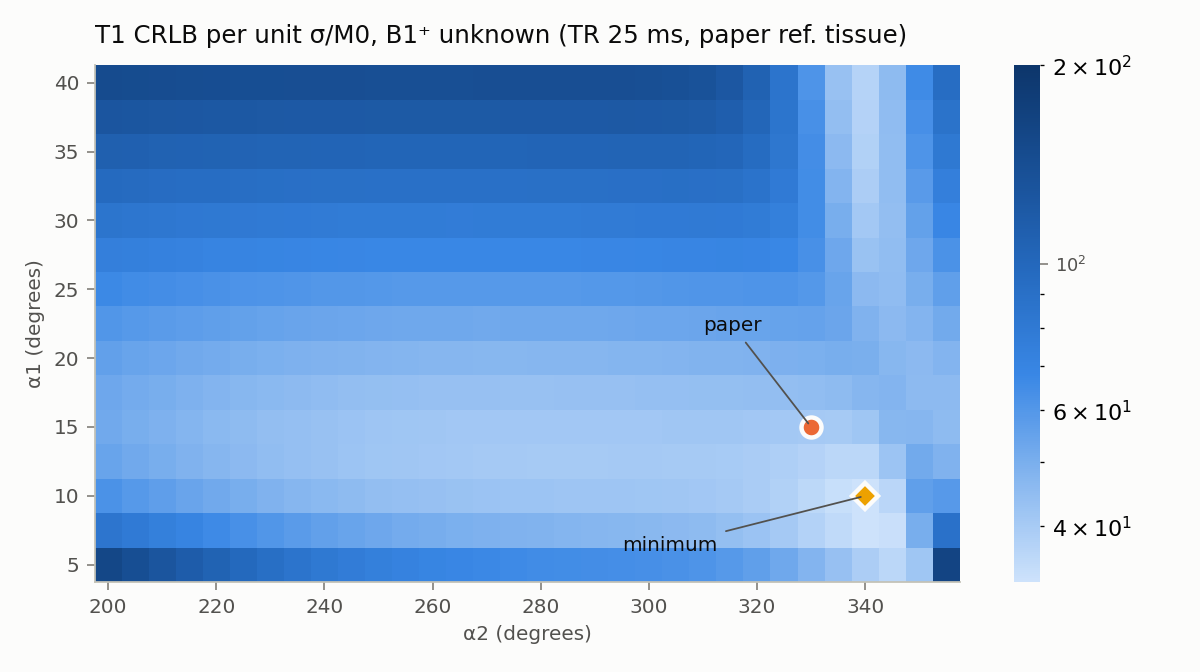
\includegraphics[width=0.78\linewidth]{crlb_flip_map.png}
\caption{$\Tone$ bound with $\Bone$ unknown over nominal $(\alpha_1,\alpha_2)$. The optimum on this grid
is $10^\circ/340^\circ$ (32.9), $19\%$ better than $15^\circ/330^\circ$.}
\label{fig:map}
\end{figure}

Over $\alpha_2^{\rm nom}\ge210^\circ$ the $\Bone$-unknown $\Tone$ bound stays within $1.5\times$ of the
$\Bone$-known one. Across $\Bone\in[0.7,1.3]$ the $\Tone$ bound is 40--65, and it grows with
$\Tone$ (15 at 300\,ms, 100 at 4000\,ms). Removing pathway $+1$ raises it from $40.5$ to $67$;
removing the echo pathway $-1$ raises it to $146$ and the $\Ttwo$ bound from $23$ to $208$.

\subsection{Global aliases}\label{sec:aliases}

Local bounds say nothing about distant parameter values that produce the same data.
\Cref{thm:uv} characterises them.

\begin{proposition}[Exact data equivalence]\label{prop:equiv}
Let both scans have the same $\TR$, and let $\Ttwo$, $\Ttwos$ and $\dw$ be fixed. Write
$u_i,v_i$ for the invariants of scan $i$ at $(\Bone,\Tone)$ and $u_i',v_i'$ at $(B_1^{+\prime},\Tone')$.
\begin{enumerate}
\item[(a)] If $u_i'=u_i$ for $i=1,2$ and $\Mzero'=\Mzero\sqrt{\tanh(\TR/2\Tone)/\tanh(\TR/2\Tone')}$, then all
  magnitudes $|S_{ijk}|$ at $(\Mzero',B_1^{+\prime},\Tone')$ equal those at $(\Mzero,\Bone,\Tone)$.
\item[(b)] If in addition $\sgn(v_1'v_2')=\sgn(v_1v_2)$, the complex signals are equal after
  replacing $\phi_0$ by $\phi_0$ or $\phi_0+\pi$.
\item[(c)] Given $u_1,u_2$, the conditions $u_i'=u_i$ are two equations in the two unknowns
  $(B_1^{+\prime},E_1')$:
  \begin{equation}
    \cos(B_1^{+\prime}\alpha_i^{\rm nom})=\frac{E_1'-u_i}{1-u_iE_1'},\qquad i=1,2.
    \label{eq:aliaseq}
  \end{equation}
\end{enumerate}
\end{proposition}
\begin{proof}
(a) \Cref{thm:uv} gives $|a_k|=|v|\,|G_k(u,E_2,\dw)|$, and \cref{lem:absv} gives
\[
  |v_i'|=\sqrt{1-u_i^2}\,\sqrt{\tanh(\TR/2\Tone')} .
\]
Hence $\Mzero'|v_i'|=\Mzero|v_i|$ for both scans with the
single stated $\Mzero'$ (both scans share $\TR$), and $\Mzero'|a_k'|=\Mzero|a_k|$ for every $k$. The echo
factors in \eqref{eq:signal} depend only on $\Ttwo$, $\Ttwos$, $\dw$ and $\phi_0$. (b) The complex
signal is $\Mzero v_i\,G_k(u_i,E_2,\dw)$ times echo factors; $v_i$ is real with
$\sgn v_i=\sgn\sin\alpha_i$ (\eqref{eq:uv}, $1-E_1\cos\alpha>0$). If $\sgn v_i'=\sgn v_i$ for both scans
the signals are equal; if both signs flip, they differ by a global factor $-1=\E^{i\pi}$,
absorbed by $\phi_0$. (c) Inverting the M\"obius map \eqref{eq:uv} in $\cos\alpha$ gives
$\cos\alpha_i=(E_1-u_i)/(1-u_iE_1)$; with $\alpha_i=\Bone\alpha_i^{\rm nom}$ this is \eqref{eq:aliaseq}.
\end{proof}

Because \eqref{eq:aliaseq} is a square system, its solutions are generically isolated and
each choice of branch of $\arccos$ in the two equations ($\pm$, plus multiples of $2\pi$) is a
candidate. Magnitude data can then be matched exactly on branches that complex data exclude
by the sign condition (b). Solving on each branch from the noise-free data gives
\cref{tab:aliases}: every alias fits to machine precision.

\begin{table}[!htbp]
\centering
\caption{Exact aliases (noise-free; relative residual $<10^{-14}$). Magnitude alias: $\alpha_2$ on
the other side of $360^\circ$. Complex alias: $\alpha_2>540^\circ$ with the same sign pattern.}
\label{tab:aliases}
\small
\begin{tabular}{cccccc}
\toprule
\multicolumn{2}{c}{Truth} & \multicolumn{2}{c}{Magnitude alias} & \multicolumn{2}{c}{Complex alias}\\
\cmidrule(lr){1-2}\cmidrule(lr){3-4}\cmidrule(lr){5-6}
$\Bone$ & $\Tone$ (ms) & $\Bone$ & $\Tone$ (ms) & $\Bone$ & $\Tone$ (ms)\\
\midrule
1.00 & 1500 & 1.199 & 1038 & 2.008 & 359\\
0.90 & 1200 & 1.350 & 527 & 1.865 & 271\\
1.05 & 850 & 1.135 & 726 & 2.100 & 204\\
0.80 & 2500 & 1.480 & 717 & 1.769 & 497\\
1.08 & 1000 & 1.102 & 960 & 2.160 & 240\\
\bottomrule
\end{tabular}
\end{table}

The complex aliases need $\Bone\approx1.8$--$2.2$ and are excluded by the assumption
$\alpha_2^{\rm nom}\Bone\le540^\circ$ of~\cite{cheng2019}, i.e.\ $\Bone<1.64$; our fits impose this bound.
The magnitude aliases lie at $\Bone\approx1.1$--$1.5$, inside the physiological range, and
require one bit of phase information (\cref{sec:magnitude}). As $\alpha_2^{\rm eff}\to360^\circ$ the
true and alias solutions merge (last row). None of this is visible in local bounds.

\subsection{Information in magnitude data}\label{sec:rician}

A magnitude $m=|S+n|$ is Rician with amplitude $A=|S|$. Its Fisher information about $A$ is
$g(A/\sigma)/\sigma^2$ with
\begin{equation}
  g(a)=\mathbb E\Bigl[x^2\,\frac{I_1(xa)^2}{I_0(xa)^2}\Bigr]-a^2,\qquad x=m/\sigma
  \label{eq:rician}
\end{equation}
(\cref{app:rician}); $g$ increases from $0$ to $1$ ($g(0.5)=0.20$, $g(2)=0.85$, $g(5)=0.98$). The
information about the five magnitude parameters is
$\Fi_{\rm mag}=\sigma^{-2}\sum_jg(A_j/\sigma)\nabla A_j\nabla A_j^{\mathsf T}$ with
$\nabla A_j=\Re(\overline{S_j}\nabla S_j)/A_j$. For the published protocol and the reference
tissue the weakest amplitude is $0.0074\,\Mzero$, so even at SNR$(\Mzero)=300$ every measurement has
$A/\sigma\ge2.2$, and the magnitude bounds equal the complex bounds to within $0.5\%$ for $\Tone$,
$\Bone$, $\Ttwo$ and $\Mzero$ at SNR 300, 1000 and 3000. Discarding the phase loses essentially no
local information; it loses the global bit of \cref{prop:equiv}(b).

\section{Maximum-likelihood estimation}\label{sec:ml}

\subsection{Estimator}

Stack the real and imaginary parts of all 18 complex measurements of a voxel into
$y\in\mathbb R^{36}$ and the model \eqref{eq:signal} into $s(\theta)$. Under the Gaussian noise
model the negative log-likelihood is $\|r(\theta)\|^2/(2\sigma^2)$ with $r=s(\theta)-y$, so the ML
estimate is the nonlinear least-squares solution $\hat\theta=\arg\min_\theta\|r(\theta)\|^2$,
independent of $\sigma$. The model is the exact steady state \eqref{eq:iso}, so the estimator
and the CRLB use the same forward model.

\paragraph{Constraints.} The fit is a projected Levenberg--Marquardt (LM) iteration. After
every step the parameters are projected onto the physical domain of the Lorentzian model,
$\log\Ttwos\le\log\Ttwo$ ($\Rtwop\ge0$), and onto a box $\Bone\in[\E^{-1},540/330]$,
$\Tone\in[10,20\,000]$\,ms, $\Ttwo\in[1,5000]$\,ms. The upper $\Bone$ bound is the assumption
$\alpha_2\le540^\circ$ of~\cite{cheng2019}; it excludes the exact complex alias of
\cref{prop:equiv} by construction. Active constraints are recorded per voxel; such estimates
are not locally unbiased and fall outside the interior CRLB.

\paragraph{Initialisation.} Magnitude parameters and $\dw$ come from a sequential estimator;
the global phase has a closed-form optimum for fixed remaining parameters,
$\phi_0^{(0)}=\arg\bigl(\sum S_{ijk}\overline{S^{(0)}_{ijk}}\bigr)$, where $S^{(0)}$ is the model at the
initial values with $\phi_0=0$.

\paragraph{Iteration.} With $J=\partial r/\partial\theta$ (exact, \cref{sec:jacobian}),
\begin{equation}
  \bigl(J^{\mathsf T}J+\lambda\,\mathrm{diag}(J^{\mathsf T}J)\bigr)\Delta=-J^{\mathsf T}r,\qquad
  \theta\leftarrow\Pi(\theta+\Delta),
\end{equation}
where $\Pi$ is the projection. A step is accepted if it lowers $\|r\|^2$ ($\lambda\leftarrow0.3\lambda$),
otherwise rejected ($\lambda\leftarrow10\lambda$); $\lambda_0=10^{-2}$, $\lambda\in[10^{-9},10^9]$, 40 iterations.
Marquardt's diagonal scaling makes the step invariant to rescaling individual parameters. A
parameter held fixed (e.g.\ a given $\Bone$ map) has its Jacobian column removed and a unit
diagonal, so that $\Delta=0$ for it. For zero-residual (noise-free) problems with a nonsingular
Jacobian, Gauss--Newton converges locally quadratically, and noise-free fits recover the
parameters to $10^{-15}$; with noise the residual at the solution is nonzero and the local
convergence is in general linear, with a rate set by the residual and the model curvature.

\paragraph{Multiple starts.} Nonlinear least squares can stop at a local minimum: across the
$360^\circ$ branch, at the branch edge where scan 2 vanishes, or along the weak direction of
\cref{fig:eigen}. We run four starts---the model-fit estimate, the analytic inverse where
valid, and the model-fit estimate with $\Tone$ replaced by 700 and by 2000\,ms---and keep the
lowest final cost. In simulation the global optimum can be checked: a final cost above the
cost at the true parameters is certainly not the ML estimate.

\paragraph{Is one start enough?} On 2000 voxels with random tissue
($\Tone$ 600--3000\,ms, $\Ttwo$ 40--140\,ms, $\Ttwos/\Ttwo$ 0.6--0.95, $\Bone$ 0.85--1.15), a single start
ends at a higher cost than the best of four in \StartWorseThreeHundred\% of voxels at
SNR$(\Mzero)=300$ (median $|\Delta\log\hat\Tone|=\StartMedianThreeHundred$, maximum \StartMaxThreeHundred)
and \StartWorseThousand\% at SNR 1000. A $\chi^2$ test on the final cost (99.9\,\% quantile,
29 degrees of freedom) flags only \StartFlaggedThreeHundred\% and \StartFlaggedThousand\% of
these, respectively. One start with a cost check is therefore not sufficient; we use four
starts throughout, which the exact Jacobian makes affordable.

\subsection{Efficiency}

\Cref{tab:mc,tab:mcb1,tab:mcdiag} compare complex ML with the analytic inverse, a sequential
model-fit baseline (the same steps with $\Bone$, $\Tone$, $\Mzero$ fitted to the FID and echo
amplitudes of both scans) and the CRLB, on 1000 noise realisations of the reference tissue.
All ratios use ordinary standard deviations; the Monte Carlo standard error of an SD from
1000 samples is about $2\%$. (These runs used the box $\Bone\le\E$; for the published protocol no
estimate reached it, so the results are the same with the $540/330$ cap.)

\begin{table}[h]
\centering
\caption{Monte Carlo robust standard deviation (\%) of the log-estimates, 1000 noise realisations, reference tissue, $\Bone=1$. SNR is relative to $\Mzero$ (peak image SNR $\approx0.088\times$). Last column: fraction of voxels with undefined $\Tone$.}
\label{tab:mc}
\small
\begin{tabular}{lllccccc}
\toprule
Protocol & SNR$(\Mzero)$ & Estimator & $\Tone$ & $\Bone$ & $\Ttwo$ & $\Mzero$ & $\Tone$ undefined\\
\midrule
$15^\circ/330^\circ$ & 300 & CRLB & 13.5 & 1.0 & 7.7 & 6.3 & --\\
 &  & Joint ML & 13.7 & 0.9 & 7.5 & 6.0 & 0.0\%\\
 &  & Model fit & 90.7 & 3.7 & 36.8 & 56.9 & 0.0\%\\
 &  & Analytic inverse~\cite{cheng2019} & 102.6 & 46.1 & 37.0 & 57.1 & 1.9\%\\
 &  & Analytic inverse, $\Bone$ given & 35.9 & -- & -- & 23.3 & 1.9\%\\
\midrule
$15^\circ/330^\circ$ & 1000 & CRLB & 4.1 & 0.3 & 2.3 & 1.9 & --\\
 &  & Joint ML & 3.9 & 0.3 & 2.5 & 1.9 & 0.0\%\\
 &  & Model fit & 11.4 & 1.3 & 11.0 & 8.5 & 0.0\%\\
 &  & Analytic inverse~\cite{cheng2019} & 12.7 & 1.5 & 11.2 & 7.6 & 0.0\%\\
 &  & Analytic inverse, $\Bone$ given & 10.7 & -- & -- & 6.5 & 0.0\%\\
\midrule
$15^\circ/330^\circ$ & 3000 & CRLB & 1.4 & 0.1 & 0.8 & 0.6 & --\\
 &  & Joint ML & 1.3 & 0.1 & 0.8 & 0.6 & 0.0\%\\
 &  & Model fit & 4.0 & 0.4 & 3.8 & 2.9 & 0.0\%\\
 &  & Analytic inverse~\cite{cheng2019} & 4.4 & 0.4 & 3.7 & 2.6 & 0.0\%\\
 &  & Analytic inverse, $\Bone$ given & 3.9 & -- & -- & 2.2 & 0.0\%\\
\midrule
$15^\circ/30^\circ$ & 1000 & CRLB & 210.6 & 102.3 & 2.3 & 104.8 & --\\
 &  & Joint ML & 211.7 & 103.7 & 2.2 & 105.3 & 0.0\%\\
 &  & Model fit & 287.6 & 138.0 & 11.0 & 149.0 & 0.0\%\\
\midrule
$15^\circ/30^\circ$ & 3000 & CRLB & 70.2 & 34.1 & 0.8 & 34.9 & --\\
 &  & Joint ML & 77.1 & 37.3 & 0.7 & 38.1 & 0.0\%\\
 &  & Model fit & 225.6 & 109.7 & 3.8 & 113.9 & 0.0\%\\
\bottomrule
\end{tabular}
\end{table}


\begin{itemize}
\item \textbf{Where its assumptions hold, ML attains the bound.} At SNR 1000 and 3000 the
  SD/CRLB ratio is 0.99--1.02 for $\Tone$, $\Bone$, $\Ttwo$ and $\Mzero$, the bias is below $10^{-3}$ in
  log units, at most $0.3\%$ of estimates touch a constraint, and no voxel fails the cost
  check. The published protocol can separate $\Bone$ and $\Tone$.
\item \textbf{At SNR 300 the comparison is approximate.} The ratio is 1.00 for $\Bone$ and 0.95
  for $\Tone$, but $\Rtwop\ge0$ is active in $19.5\%$ of voxels (true $\Rtwop$ is small); those estimates
  are biased, which is how the $\Tone$ SD can fall slightly below the bound.
\item \textbf{The analytic inverse is 3.2--7.1 times above the bound} for $\Tone$, with bias
  $+0.44$ in $\log\Tone$ and $1.9\%$ undefined estimates at SNR 300; $\Bone$ is 4.8--28 times above.
  Given the true $\Bone$, its $\Tone$ step is 1.9--2.8 times above its matched bound (scan 1,
  $\Bone$ known: 57.1). The model-fit baseline, which shares the sequential structure but not
  the closed forms, behaves similarly, so the loss comes from the sequential structure.
\item \textbf{The small-angle control supports no efficiency claim.} For $15^\circ/30^\circ$,
  $10$--$35\%$ of ML estimates are on a box bound and biased; the bound itself is of order one
  in log units ($2.1$ at SNR 1000, a one-sigma factor of about 8), while $\Ttwo$ is unaffected.
\end{itemize}

\section{Least squares on magnitude images}\label{sec:magnitude}

The published inverse works with magnitudes, made real-valued by the sign convention of its
Eq.~18. A direct alternative is to fit the model magnitudes,
\begin{equation}
  \hat\theta=\arg\min_\theta\sum_j\bigl(|y_j|-|s_j(\theta)|\bigr)^2,
  \label{eq:magls}
\end{equation}
over $\theta=(\log\Mzero,\log\Bone,\log\Tone,\log\Ttwo,\log\Ttwos)$ with the same projected LM iteration,
constraints and four starts as complex ML. This is not maximum likelihood for magnitude data,
which are Rician: it ignores the noise floor $\mathbb E|y|-A\approx\sigma^2/(2A)$, which for the weakest
amplitude of the reference tissue is $10\%$ at SNR 300, $1\%$ at SNR 1000 and $0.1\%$ at SNR 3000.
\Cref{sec:rician} showed that magnitudes carry essentially all the local information; this
section concerns the global bit they lose.

\subsection{Why a magnitude fit needs the branch test and complex ML does not}

\paragraph{1. Magnitudes lose the sign of $\sin\alpha$.} By \cref{thm:uv} and \cref{lem:absv}
the magnitudes of scan $i$ determine $u_i$ and $\Mzero|v_i|=\Mzero\sqrt{1-u_i^2}\tanh(\TR/2\Tone)$, i.e.\
$\cos\alpha_i$ for any trial $E_1$, but not the sign of $\sin\alpha_i$. Equivalently, $|a_k(\alpha)|$ is
even and $2\pi$-periodic in $\alpha$, hence symmetric about every multiple of $180^\circ$.

\paragraph{2. This produces an exact alias in the physiological range.} By
\cref{prop:equiv}(a,c) the magnitude data at $(\Mzero,\Bone,\Tone)$ are reproduced exactly at every
solution $(B_1^{+\prime},E_1')$ of \eqref{eq:aliaseq}, with $\Mzero'$ set by part (a). The branch
$\alpha_2=360^\circ+x'$ admits such a solution: for the reference tissue $(1,1500\,\mathrm{ms},1)$ and
$(1.199,1038\,\mathrm{ms},0.832)$ give the same 18 magnitudes to machine precision
(\cref{tab:aliases}). The alias is close to the small-angle scaling
($1500/1.199^2=1043$) but exact.

\paragraph{3. It is a symmetry of the magnitude likelihood, not a noise effect.} The alias
exists for every parameter value, so the map $\theta\mapsto|s(\theta)|$ takes the same values on two
separate sheets of parameter space. Any likelihood that depends on the data only through
magnitudes, Gaussian or Rician, has two equal global maxima for every noise realisation. We
verified this directly: fitting noisy magnitudes on each side of $360^\circ$ gives final costs
that agree to a median relative difference of $10^{-12}$ at SNR 300, 1000 and 3000. No SNR
resolves it, and the local CRLB, identical on both sheets, cannot detect it. An
unconstrained magnitude fit returns the maximum nearest its starting point: in
\cref{tab:mag} it chose the wrong branch in 47, 3 and \MagWrongThree{} of 1000 voxels at SNR
300, 1000 and 3000, and in 13, 3 and 0 when the same fits were run with the exact Jacobian,
which takes slightly different paths. The counts describe the optimiser, not the data.

\paragraph{4. Complex data carry the missing bit.} By \cref{prop:period},
$a_k(-\alpha)=-a_k(\alpha)$, so moving $\alpha_2$ from $360^\circ-x$ to $360^\circ+x'$ flips the sign of every
scan-2 signal relative to scan 1 (\cref{prop:equiv}(b)). A single $\phi_0$ and a single $\dw$ are
shared by both scans, so the relative sign cannot be absorbed. The best complex fit
restricted to $360^\circ<\alpha_2<540^\circ$ moves to the edge $\alpha_2=360^\circ$, where scan 2 vanishes, and
leaves the entire scan-2 signal ($0.144\,\Mzero$) as residual: its cost exceeds the true-branch
cost by $1.9\times10^3\sigma^2$ at SNR 300 ($2.1\times10^4\sigma^2$ at SNR 1000), a likelihood ratio of about
$\E^{-935}$ or smaller. Complex ML selects the correct branch automatically.

\paragraph{5. The FID-sign test restores the bit.} The test of~\cite{cheng2019},
\begin{equation}
  \sgn\,\Re\sum_jS_{1j0}\overline{S_{2j0}}=\sgn(\sin\alpha_1\sin\alpha_2),
  \label{eq:fidsign}
\end{equation}
uses only the sign of the relative phase of the two FID images (it follows from
$a_0\propto v\propto\sin\alpha$ and the shared echo phases). In the magnitude fit it becomes a
constraint: $\Bone$ is confined to the interval between consecutive zeros of
$\sin(\Bone\alpha_i^{\rm nom})$ on which $\sin\alpha_1\sin\alpha_2$ has the measured sign; a start on the wrong
side is reflected across the nearest zero, where $|a_k|$ is symmetric, and every step is
projected back into the interval (\cref{alg:branch}).

\paragraph{6. What the test cannot do.} Branches with the same sign pattern (the complex
aliases, $\alpha_2>540^\circ$) are invisible to the test and to complex ML; the range bound excludes
them. Near $\alpha_2^{\rm eff}=360^\circ$ the scan-2 FID vanishes and the sign is unreliable, but the two
branches merge there, so a wrong decision costs little. Both the test and complex ML need the
relative phase of the two scans to be preserved: the same receiver phase and coil combination
and no motion or $B_0$ drift between the sequential acquisitions. With an unknown phase per
scan, complex ML would lose the relative sign and the alias would reappear for complex data
too.

\subsection{Comparison on identical data}

\Cref{tab:mag} compares the analytic inverse, magnitude least squares without and with the
FID-sign constraint, and complex ML on the noise realisations of \cref{tab:mc}.

\begin{table}[h]
\centering
\caption{Magnitude versus complex estimation on identical data (paper protocol, reference tissue, 1000 realisations). SD and mean of the log-estimates; bounds for complex data and for magnitude (Rician) data. Last column: voxels on the wrong side of $\alpha_2=360^\circ$ (``wrong'').}
\label{tab:mag}
\footnotesize
\setlength{\tabcolsep}{4pt}
\begin{tabular}{llccccc}
\toprule
SNR & & $\Tone$ SD & $\Tone$ mean & $\Bone$ SD & $\Ttwo$ SD & wrong\\
\midrule
300 & CRLB complex/Rician & 0.1350/0.1356 & & 0.0097/0.0098 & 0.0769/0.0771 & \\
 & Analytic inverse~\cite{cheng2019} & 0.9587 & +0.445 & 0.2695 & 0.5060 & --\\
 & Magnitude LS & 0.1909 & -0.030 & 0.0692 & 0.0743 & 47\\
 & Magnitude LS + FID sign & 0.1251 & -0.005 & 0.0094 & 0.0742 & 0\\
 & Complex ML & 0.1281 & -0.007 & 0.0097 & 0.0749 & --\\
\midrule
1000 & CRLB complex/Rician & 0.0405/0.0405 & & 0.0029/0.0029 & 0.0231/0.0231 & \\
 & Analytic inverse~\cite{cheng2019} & 0.2072 & +0.036 & 0.0657 & 0.1180 & --\\
 & Magnitude LS & 0.0457 & +0.000 & 0.0104 & 0.0231 & 3\\
 & Magnitude LS + FID sign & 0.0409 & +0.001 & 0.0029 & 0.0231 & 0\\
 & Complex ML & 0.0411 & +0.001 & 0.0029 & 0.0231 & --\\
\midrule
3000 & CRLB complex/Rician & 0.0135/0.0135 & & 0.0010/0.0010 & 0.0077/0.0077 & \\
 & Analytic inverse~\cite{cheng2019} & 0.0425 & +0.001 & 0.0046 & 0.0373 & --\\
 & Magnitude LS & 0.0136 & +0.000 & 0.0010 & 0.0076 & 0\\
 & Magnitude LS + FID sign & 0.0136 & +0.000 & 0.0010 & 0.0076 & 0\\
 & Complex ML & 0.0136 & +0.000 & 0.0010 & 0.0076 & --\\
\bottomrule
\end{tabular}
\end{table}


With the branch test, magnitude least squares has SD/CRLB within the Monte Carlo error of
complex ML at every SNR and no wrong-branch voxels; the Rician floor adds a small bias at SNR
300 ($-0.005$ in $\log\Tone$). Without it, wrong-branch voxels dominate the $\Bone$ error (SD up to
seven times the robust spread) and bias $\Tone$ by about $(\Bone)^{-2}$. The analytic inverse, which uses
the same magnitudes and the same FID sign, is 3--7 times worse for $\Tone$ and up to 28 times
for $\Bone$: since magnitudes carry essentially all the local information and a joint magnitude
fit extracts it, its loss is algorithmic.

\section{Exact Jacobians by implicit differentiation}\label{sec:jacobian}

Both least-squares estimators spend nearly all their time forming Jacobians: $36\times7$ per
voxel for complex data and $18\times5$ for magnitudes. Reverse-mode differentiation
(back-propagation) produces one \emph{row} per backward pass and would need 36 or 18 passes;
forward mode produces one \emph{column} per pass, 7 or 5 passes, and forward differences are
an inexact version of it. The structure of the steady state allows something cheaper.

\subsection{Differentiating the steady state}

With RF phase $0$ the post-pulse steady state of one isochromat solves \eqref{eq:iso},
\begin{equation}
  A\mathbf M=\mathbf b,\qquad A=I-RQ,\qquad Q=R_z(\psi)\,\mathrm{diag}(E_2,E_2,E_1),\qquad
  \mathbf b=(1-E_1)R\hat{\mathbf z},
\end{equation}
with $R=R_x(\alpha)$ and $\dw=0$ (\cref{prop:offres}). For $x\in\{\alpha,E_1,E_2\}$,
\begin{equation}
  \frac{\partial\mathbf M}{\partial x}=A^{-1}\Bigl(\frac{\partial\mathbf b}{\partial x}-\frac{\partial A}{\partial x}\mathbf M\Bigr),
  \label{eq:implicit}
\end{equation}
so the inverse used for the solution serves all three derivatives. With $R'=\partial R_x/\partial\alpha$,
$\Pi_z=\mathrm{diag}(0,0,1)$, $\Pi_{xy}=\mathrm{diag}(1,1,0)$ and $R_z\Pi_z=\Pi_z$,
\begin{align}
  \frac{\partial A}{\partial\alpha}&=-R'Q, &\frac{\partial\mathbf b}{\partial\alpha}&=(1-E_1)R'\hat{\mathbf z},\nonumber\\
  \frac{\partial A}{\partial E_1}&=-R\Pi_z, &\frac{\partial\mathbf b}{\partial E_1}&=-R\hat{\mathbf z},\\
  \frac{\partial A}{\partial E_2}&=-RR_z(\psi)\Pi_{xy}, &\frac{\partial\mathbf b}{\partial E_2}&=\mathbf0,\nonumber
\end{align}
and the three right-hand sides of \eqref{eq:implicit} are
\begin{equation}
  (1-E_1)R'\hat{\mathbf z}+R'Q\mathbf M,\qquad -R\hat{\mathbf z}+R\hat{\mathbf z}\,M_z,\qquad RR_z(\psi)\Pi_{xy}\mathbf M .
\end{equation}
There are $N\times n_{\rm iso}$ systems per scan; batched general solvers carry a large per-matrix
overhead at size $3\times3$, so $A^{-1}=\mathrm{adj}(A)/\det A$ is formed explicitly (nine cofactors
and one determinant, elementwise over the batch). $A$ is invertible whenever $E_1,E_2<1$.
Pathway amplitudes are discrete Fourier coefficients over the isochromats, and the transform
is linear, so $\partial a_k/\partial x$ is the same FFT of $\partial m_\perp/\partial x$; for magnitudes
$\partial|a_k|/\partial x=\Re(\overline{a_k}\,\partial a_k/\partial x)/|a_k|$.

\subsection{Chain rule}

With $\tau=t+k\TR$, $\Phi=\phi_0+\dw\tau$, $D=\exp(-t/\Ttwo-\Rtwop|\tau|)$, $\Rtwop=1/\Ttwos-1/\Ttwo$,
$S=\Mzero a_kD\E^{i\Phi}$ and $\partial\alpha/\partial\log\Bone=\alpha$, $\partial E_1/\partial\log\Tone=E_1\TR/\Tone$,
$\partial E_2/\partial\log\Ttwo=E_2\TR/\Ttwo$:
\begin{align}
  \frac{\partial S}{\partial\log\Mzero}&=S, &
  \frac{\partial S}{\partial\log\Bone}&=\Mzero D\E^{i\Phi}\alpha\frac{\partial a_k}{\partial\alpha},\nonumber\\
  \frac{\partial S}{\partial\log\Tone}&=\Mzero D\E^{i\Phi}\frac{E_1\TR}{\Tone}\frac{\partial a_k}{\partial E_1}, &
  \frac{\partial S}{\partial\log\Ttwo}&=\Mzero D\E^{i\Phi}\frac{E_2\TR}{\Ttwo}\frac{\partial a_k}{\partial E_2}+S\frac{t-|\tau|}{\Ttwo},\\
  \frac{\partial S}{\partial\log\Ttwos}&=S\frac{|\tau|}{\Ttwos}, &
  \frac{\partial S}{\partial\dw}&=i\tau S,\qquad\frac{\partial S}{\partial\phi_0}=iS .\nonumber
\end{align}
The second term of $\partial S/\partial\log\Ttwo$ combines $\E^{-t/\Ttwo}$ and the coupling through $\Rtwop$
($\partial\Rtwop/\partial\log\Ttwo=1/\Ttwo$). For magnitudes, $|a_k|$ replaces $a_k$ and the phase terms are dropped.

\subsection{Levenberg--Marquardt with exact Jacobians}

A forward-difference iteration costs one trial evaluation plus one per parameter (8 for
complex data, 6 for magnitudes). With exact Jacobians each trial evaluation returns the
residual and its Jacobian; an accepted step thus already carries the Jacobian of the next
iteration, and a rejected one keeps the current Jacobian. Each iteration costs one explicit
inverse and four right-hand sides per isochromat. Exact derivatives also make single
precision usable: forward differences in float32 would need steps of order $10^{-3}$, whereas
the implicit Jacobian is accurate to about $10^{-6}$. A small Jacobian error changes the
convergence path but not the solution, which is set by the residual.

\subsection{Verification and benchmark}

The implicit Jacobians agree with automatic differentiation of the reference model to
$6\times10^{-15}$ (magnitude) and $3\times10^{-16}$ (complex) in double precision and to $10^{-6}$ in single
precision. \Cref{tab:bench} lists wall times on 4096 voxels with random tissue
($\Tone$ 600--3000\,ms, $\Ttwo$ 40--120\,ms, $\Bone$ 0.8--1.1), SNR$(\Mzero)=1000$, one start and 15
iterations (15 and 40 iterations differ by less than $10^{-9}$ in $\log\Tone$), on a laptop CPU with 8
threads.

\begin{table}[!htbp]
\centering
\caption{Fitting time and agreement with the forward-difference float64 reference (largest
$|\Delta\log\hat\Tone|$ over 4096 voxels; the noise-induced spread is $0.164$ for magnitudes and $0.163$ for
complex data).}
\label{tab:bench}
\small
\begin{tabular}{llcccc}
\toprule
Fit & Jacobian, precision, isochromats & ms/voxel & $256^2$ slice & speed-up & max $|\Delta\log\hat\Tone|$\\
\midrule
Magnitude & finite differences, f64, 256 & 15.0 & 16.4 min & 1.0 & reference\\
 & implicit, f64, 256 & 1.41 & 1.5 min & 10.7 & $1.6\times10^{-5}$\\
 & implicit, f64, 128 & 0.73 & 0.8 min & 20.6 & $1.6\times10^{-5}$\\
 & implicit, f32, 256 & 0.74 & 0.8 min & 20.2 & $1.2\times10^{-3}$\\
 & implicit, f32, 128 & 0.44 & 0.5 min & 33.7 & $1.0\times10^{-3}$\\
\midrule
Complex ML & finite differences, f64, 256 & 19.2 & 21.0 min & 1.0 & reference\\
 & implicit, f64, 256 & 1.55 & 1.7 min & 12.4 & $1.4\times10^{-5}$\\
 & implicit, f64, 128 & 0.83 & 0.9 min & 23.2 & $1.4\times10^{-5}$\\
 & implicit, f32, 256 & 0.90 & 1.0 min & 21.3 & $1.2\times10^{-3}$\\
 & implicit, f32, 128 & 0.56 & 0.6 min & 34.4 & $1.2\times10^{-3}$\\
\bottomrule
\end{tabular}
\end{table}

The exact Jacobian alone gives a factor of 10--12, more than the reduction from 6--8
evaluations to one would suggest, because the explicit inverse also avoids per-matrix solver
overhead. Halving the isochromats and moving to float32 each roughly halve the time again,
changing estimates by at most $10^{-3}$ in $\log\hat\Tone$ ($<1\%$ of the noise spread). With the full
Monte Carlo scripts, the implicit Jacobian reproduces the reference results to every
displayed digit for the published protocol and cuts a 25-minute run to 88\,s (22\,s in float32
with 128 isochromats and 15 iterations).

\subsection{Implications}

\begin{itemize}
\item \textbf{Whole-brain feasibility.} With four starts a $256\times256$ slice takes about 2--3 minutes
  in float64 and about 1 minute in float32 on this CPU; a whole brain (about 160 slices,
  masked) a few hours, and minutes on a GPU, since every operation is a batched elementwise
  or FFT operation.
\item \textbf{Uncertainty maps at no extra cost.} The Jacobian at the solution gives the local CRLB,
  $\sqrt{\mathrm{diag}(J^{\mathsf T}J)^{-1}}\,\sigma$, per voxel. \Cref{sec:phantom} shows these maps are
  calibrated where the estimator is efficient.
\item \textbf{Protocol optimisation.} The Fisher information of a protocol is one Jacobian
  evaluation; gradients with respect to protocol parameters (TR, flip angles, echo times) can
  be obtained the same way, enabling direct CRLB-based design rather than grid searches.
\item \textbf{Training data and learned estimators.} Simulated signals with exact Jacobians and
  bounds are cheap, for neural networks (\cref{sec:future}) and for evaluating them against
  the CRLB.
\item \textbf{Hierarchical estimation.} An empirical-Bayes EM algorithm (\cref{sec:future}) needs a
  MAP fit and a Laplace covariance per voxel and class at every iteration; both come directly
  from this machinery.
\item \textbf{Robust starts.} Because one start is not enough (\cref{sec:ml}), multiple starts are
  the dominant cost; making each fit 10--34 times cheaper is what makes four starts routine.
\end{itemize}

\section{Digital phantom}\label{sec:phantom}

\subsection{Phantom and simulated acquisition}

The phantom is a $256\times256$ axial-slice-like arrangement of tissue classes
(\cref{fig:phantom}): an outer CSF rim, cortical grey matter with a gyrated boundary, white
matter, two lateral ventricles, two deep grey-matter nuclei and a white-matter lesion, in
total \Voxels{} voxels (\cref{tab:tissues}). Each class carries 3\,T-typical relaxation values,
modulated by a smooth random texture of $3\%$ (log scale) so that tissues are not uniform.
Smooth fields model the transmit field (centre brightening, $\Bone=0.87$--$1.15$, so that about a
quarter of the voxels have $\alpha_2>360^\circ$ and a ring of voxels has $\alpha_2\approx360^\circ$), the
off-resonance (a quadratic background of $\pm20$\,Hz and a frontal hot spot of about $+50$\,Hz),
the receive sensitivity ($\pm15\%$) and the receive phase.

\begin{table}[!htbp]
\centering
\caption{Phantom tissue classes (before the $3\%$ texture).}
\label{tab:tissues}
\small
\begin{tabular}{lrrrrr}
\toprule
Tissue & $\Tone$ (ms) & $\Ttwo$ (ms) & $\Ttwos$ (ms) & PD & voxels\\
\midrule
CSF & 4000 & 1500 & 900 & 1.00 & 5614\\
GM & 1350 & 90 & 60 & 0.82 & 14\,782\\
WM & 850 & 66 & 50 & 0.69 & 16\,196\\
deep GM & 1130 & 58 & 40 & 0.75 & 1104\\
lesion & 1500 & 120 & 80 & 0.85 & 180\\
\bottomrule
\end{tabular}
\end{table}

\begin{figure}[!htbp]
\centering
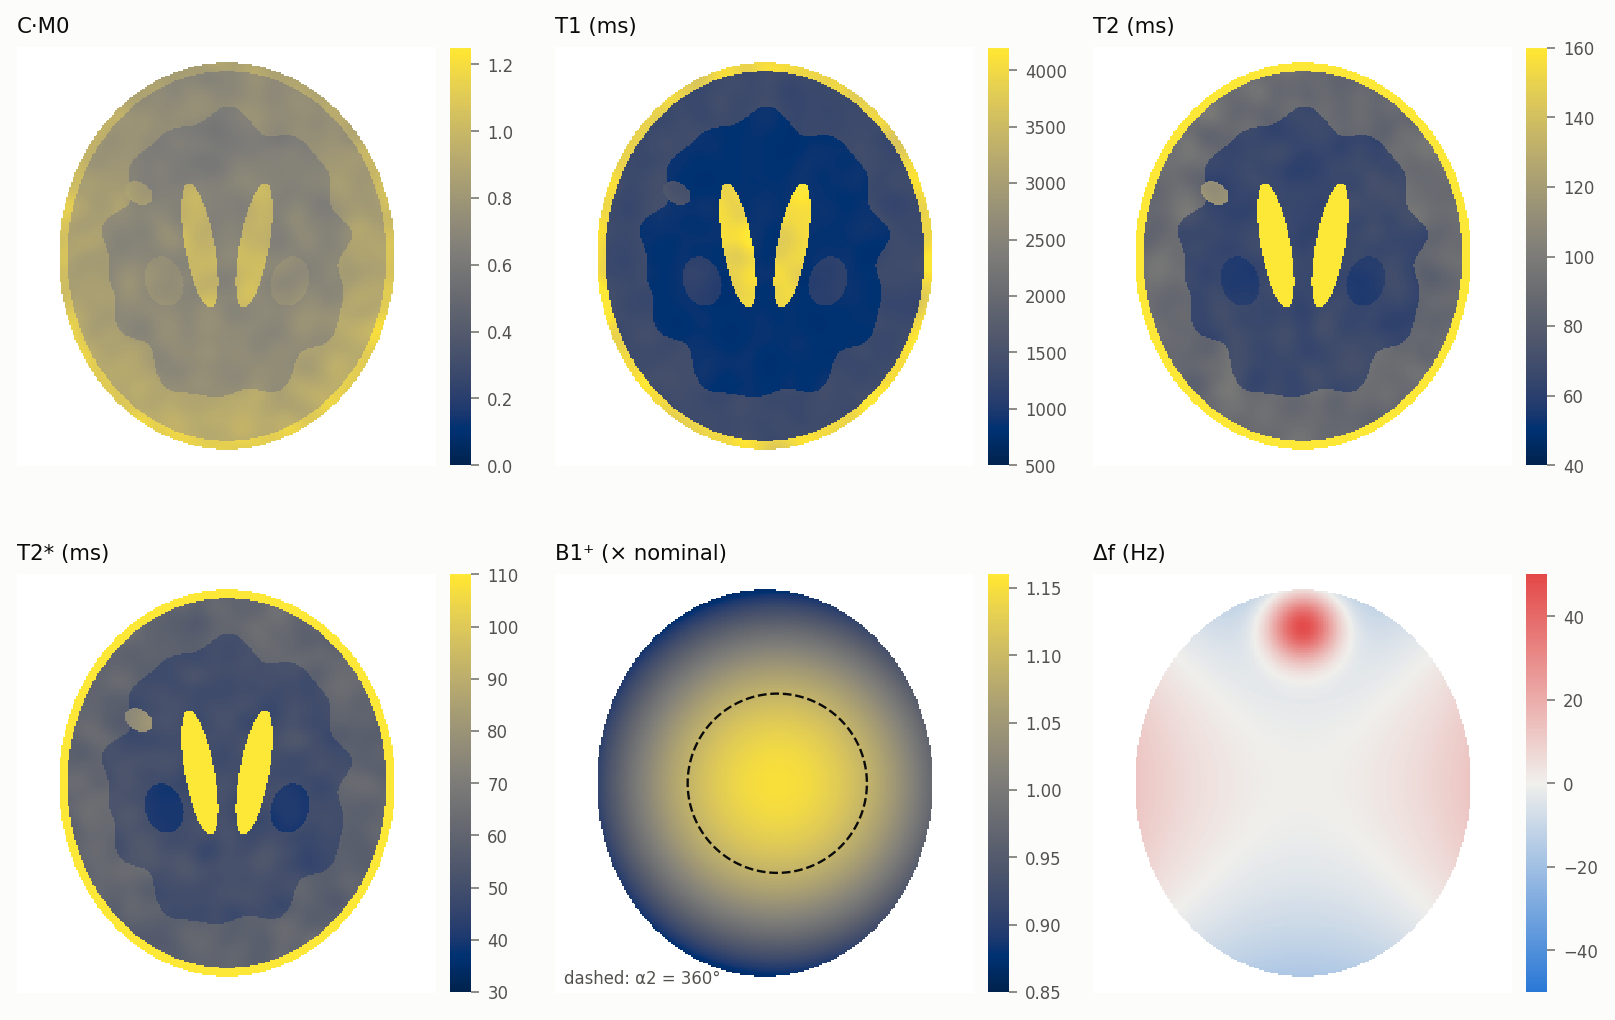
\includegraphics[width=0.92\linewidth]{phantom_truth.png}
\caption{True parameter maps. The dashed contour marks $\alpha_2=330^\circ\Bone=360^\circ$.}
\label{fig:phantom}
\end{figure}

Images are generated voxel by voxel with the forward model \eqref{eq:signal} (512
isochromats; no partial volume within a voxel) and complex Gaussian noise with
$\sigma=1/\mathrm{SNR}(\Mzero)$, for SNR$(\Mzero)=1000$ and $300$ ($\Mzero$ ranges from 0.6 to 1.2). Two
acquisitions are simulated (\cref{fig:images}):
\begin{itemize}
\item \textbf{Scenario A}: both scans at full resolution, the per-voxel setting of
  \cref{sec:information,sec:ml,sec:magnitude};
\item \textbf{Scenario B}: the published design, in which scan 2 covers only the central
  $25\%$ of the phase-encoding lines ($k_y$), with zero filling. (In 3D the published design
  keeps $25\%\times25\%$ of $k_y$--$k_z$, a factor 16; in 2D only one phase-encoding axis can be
  truncated, a factor 4.) Noise is added before truncation, i.e.\ the same per-sample noise
  with fewer samples.
\end{itemize}

\begin{figure}[!htbp]
\centering
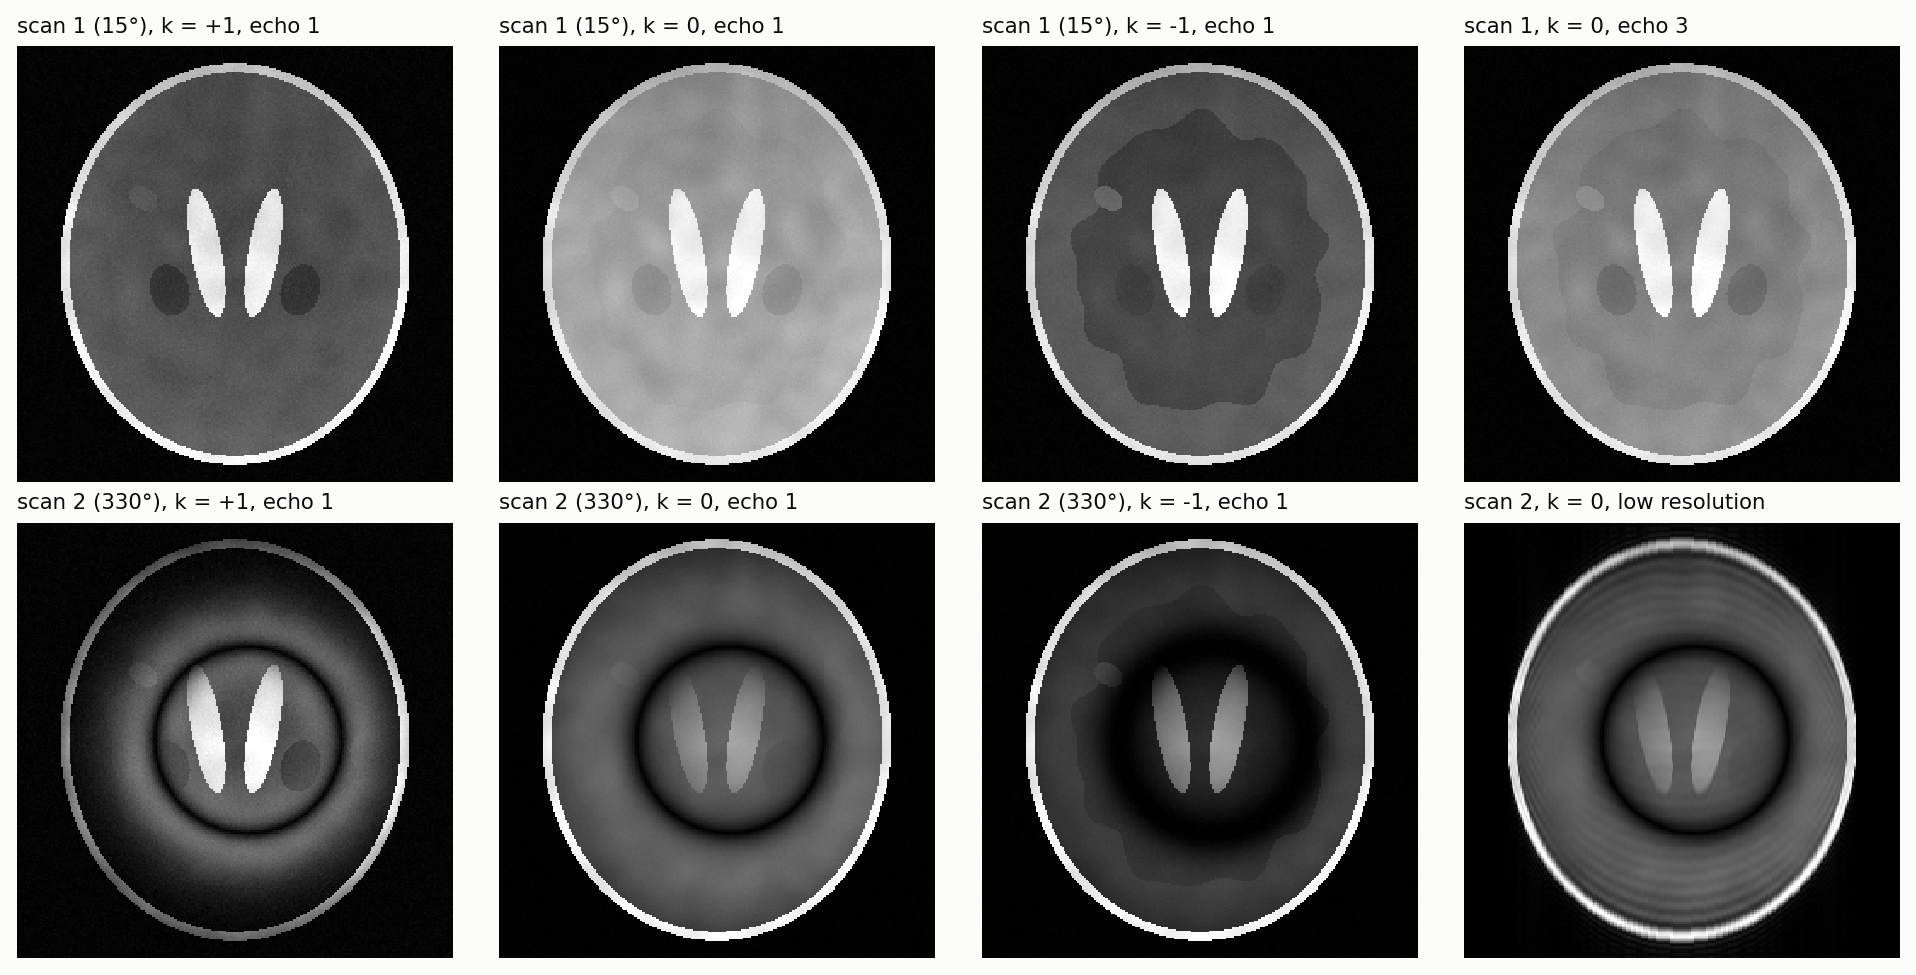
\includegraphics[width=\linewidth]{phantom_images.png}
\caption{Simulated MPME images (magnitude, SNR$(\Mzero)=1000$). The scan-2 images show the dark
ring where $\alpha_2^{\rm eff}=360^\circ$ and the signal vanishes; bottom right: the low-resolution scan 2 of
Scenario B, with truncation ringing.}
\label{fig:images}
\end{figure}

\subsection{Reconstructions}

All fits use the exact Jacobian in single precision with 128 isochromats, 25 iterations,
the $\Bone\le540/330$ bound and four starts (\cref{alg:ml}), processed in chunks of 4096 voxels.
\begin{itemize}
\item \textbf{Scenario A.} The analytic inverse (voxel-wise flip angle, no smoothing);
  complex ML; magnitude least squares with the FID-sign constraint. For the last two, a
  fifth \emph{spatial-restart} start is added after the first pass: the first-pass $\Bone$ map is
  smoothed by a robust polynomial fit, and each voxel is restarted from
  $(\Mzero\kappa,\ B^{+}_{1,\rm smooth},\ \Tone\kappa^2)$ with $\kappa=\Bone/B^{+}_{1,\rm smooth}$, i.e.\ moved along the
  near-degenerate direction of \cref{prop:scaling}; the lowest cost is kept. The neighbourhood
  only proposes a start, so every estimate remains a per-voxel likelihood maximum.
\item \textbf{Scenario B.} The paper pipeline (\cref{alg:twostage}): the flip angle from the
  two low-resolution scans by Eq.~15, a degree-4 robust polynomial fit, then $\Tone$, $\Ttwo$ and
  $\Mzero$ from full-resolution scan 1 by Eqs.~1, 16 and 17. The ML pipeline: $\Bone$ from the two
  low-resolution scans by complex ML, the same polynomial fit, then complex ML on
  full-resolution scan 1 with $\Bone$ fixed.
\end{itemize}

\paragraph{Why the spatial restart.} Without it, 324 voxels (SNR 1000) had $|\log(\hat\Tone/\Tone)|>0.3$;
321 of them lie within $3^\circ$ of $\alpha_2=360^\circ$, where scan 2 carries almost no signal and the problem
approaches the one-scan degeneracy of \cref{cor:onescan}. In 222 of the 324 the final cost
exceeded the cost at the true parameters (optimiser failures: all four starts derive from
estimators that are unreliable at $360^\circ$). The smoothed $\Bone$ map is accurate to $0.03\%$ there,
and the restart removes all optimiser failures (no voxel ends above the true-parameter cost).
The remaining large errors (53 at SNR 1000, 50 of them within $3^\circ$ of $360^\circ$) all have a cost at
or below the true one: they are genuine maxima of the likelihood, a property of the protocol
at $\alpha_2\approx360^\circ$ rather than of the estimator.

\subsection{Results}

\begin{table}[!htbp]
\centering
\caption{Phantom, SNR$(\Mzero)=1000$: median and SD of $\log(\hat\theta/\theta)$ over each tissue (bias and spread), and the fraction of voxels with an undefined estimate. Truth includes a $3\%$ smooth texture.}
\label{tab:roi1000}
\footnotesize
\setlength{\tabcolsep}{3.5pt}
\begin{tabular}{llcccccc}
\toprule
Tissue & Method & $\Tone$ median & $\Tone$ SD & $\Ttwo$ median & $\Ttwo$ SD & $\Bone$ median & undef.\,\%\\
\midrule
WM & A, analytic inverse & +0.006 & 0.298 & -0.000 & 0.145 & -0.000 & 0.0\\
 & A, complex ML & +0.001 & 0.094 & +0.001 & 0.041 & +0.000 & 0.0\\
 & A, magnitude LS + FID & -0.000 & 0.124 & +0.003 & 0.041 & +0.000 & 0.0\\
 & B, paper pipeline & +0.001 & 0.101 & -0.000 & 0.145 & +0.001 & 0.0\\
 & B, ML pipeline & +0.001 & 0.073 & -0.000 & 0.055 & -0.000 & 0.0\\
\midrule
GM & A, analytic inverse & +0.003 & 0.403 & +0.001 & 0.160 & +0.000 & 0.0\\
 & A, complex ML & +0.001 & 0.042 & +0.001 & 0.030 & +0.000 & 0.0\\
 & A, magnitude LS + FID & +0.002 & 0.042 & +0.000 & 0.030 & +0.000 & 0.0\\
 & B, paper pipeline & +0.043 & 0.117 & +0.001 & 0.160 & -0.015 & 0.0\\
 & B, ML pipeline & +0.001 & 0.065 & +0.001 & 0.051 & +0.000 & 0.0\\
\midrule
deep GM & A, analytic inverse & +0.011 & 0.321 & -0.009 & 0.141 & -0.000 & 0.0\\
 & A, complex ML & -0.000 & 0.115 & +0.000 & 0.041 & +0.000 & 0.0\\
 & A, magnitude LS + FID & -0.002 & 0.131 & +0.003 & 0.041 & +0.000 & 0.0\\
 & B, paper pipeline & +0.006 & 0.154 & -0.009 & 0.141 & -0.001 & 0.0\\
 & B, ML pipeline & +0.001 & 0.084 & -0.000 & 0.052 & -0.000 & 0.0\\
\midrule
lesion & A, analytic inverse & -0.004 & 0.119 & -0.009 & 0.167 & -0.000 & 0.0\\
 & A, complex ML & -0.007 & 0.050 & -0.005 & 0.031 & -0.000 & 0.0\\
 & A, magnitude LS + FID & -0.008 & 0.050 & -0.004 & 0.031 & -0.000 & 0.0\\
 & B, paper pipeline & -0.008 & 0.118 & -0.009 & 0.167 & +0.001 & 0.0\\
 & B, ML pipeline & +0.005 & 0.059 & -0.004 & 0.050 & +0.000 & 0.0\\
\midrule
CSF & A, analytic inverse & +0.015 & 0.650 & -0.019 & 0.802 & -0.000 & 0.1\\
 & A, complex ML & -0.001 & 0.079 & -0.000 & 0.080 & +0.000 & 0.0\\
 & A, magnitude LS + FID & -0.001 & 0.079 & -0.000 & 0.080 & +0.000 & 0.0\\
 & B, paper pipeline & +0.085 & 0.356 & -0.019 & 0.802 & -0.015 & 0.1\\
 & B, ML pipeline & -0.004 & 0.099 & +0.003 & 0.114 & -0.000 & 0.0\\
\bottomrule
\end{tabular}
\end{table}

\begin{table}[!htbp]
\centering
\caption{Phantom, SNR$(\Mzero)=300$: median and SD of $\log(\hat\theta/\theta)$ over each tissue (bias and spread), and the fraction of voxels with an undefined estimate. Truth includes a $3\%$ smooth texture.}
\label{tab:roi300}
\footnotesize
\setlength{\tabcolsep}{3.5pt}
\begin{tabular}{llcccccc}
\toprule
Tissue & Method & $\Tone$ median & $\Tone$ SD & $\Ttwo$ median & $\Ttwo$ SD & $\Bone$ median & undef.\,\%\\
\midrule
WM & A, analytic inverse & +0.015 & 0.652 & +0.003 & 0.771 & -0.002 & 1.3\\
 & A, complex ML & +0.000 & 0.230 & +0.005 & 0.138 & +0.000 & 0.0\\
 & A, magnitude LS + FID & -0.009 & 0.250 & +0.026 & 0.139 & +0.000 & 0.0\\
 & B, paper pipeline & -0.017 & 0.452 & +0.003 & 0.771 & +0.001 & 1.3\\
 & B, ML pipeline & -0.006 & 0.225 & +0.008 & 0.176 & -0.000 & 0.0\\
\midrule
GM & A, analytic inverse & +0.015 & 0.913 & +0.004 & 0.879 & +0.000 & 1.6\\
 & A, complex ML & +0.002 & 0.139 & +0.004 & 0.102 & +0.000 & 0.0\\
 & A, magnitude LS + FID & +0.013 & 0.137 & +0.001 & 0.100 & +0.002 & 0.0\\
 & B, paper pipeline & +0.027 & 0.508 & +0.004 & 0.879 & -0.016 & 1.6\\
 & B, ML pipeline & -0.000 & 0.208 & +0.009 & 0.168 & +0.000 & 0.0\\
\midrule
deep GM & A, analytic inverse & -0.018 & 0.728 & -0.023 & 0.762 & -0.002 & 5.4\\
 & A, complex ML & +0.002 & 0.287 & +0.003 & 0.170 & +0.000 & 0.0\\
 & A, magnitude LS + FID & -0.026 & 0.301 & +0.033 & 0.143 & +0.000 & 0.0\\
 & B, paper pipeline & -0.048 & 0.656 & -0.023 & 0.762 & -0.000 & 5.4\\
 & B, ML pipeline & -0.003 & 0.276 & +0.004 & 0.173 & +0.000 & 0.0\\
\midrule
lesion & A, analytic inverse & -0.032 & 0.747 & -0.028 & 0.933 & -0.001 & 1.7\\
 & A, complex ML & -0.026 & 0.161 & -0.006 & 0.100 & -0.000 & 0.0\\
 & A, magnitude LS + FID & -0.030 & 0.160 & +0.007 & 0.100 & -0.000 & 0.0\\
 & B, paper pipeline & -0.037 & 0.593 & -0.028 & 0.933 & +0.001 & 1.7\\
 & B, ML pipeline & -0.009 & 0.179 & -0.014 & 0.160 & -0.000 & 0.0\\
\midrule
CSF & A, analytic inverse & +0.047 & 1.011 & -0.054 & 1.228 & -0.010 & 17.8\\
 & A, complex ML & -0.015 & 0.275 & +0.003 & 0.280 & +0.000 & 0.0\\
 & A, magnitude LS + FID & -0.015 & 0.275 & +0.002 & 0.280 & +0.000 & 0.0\\
 & B, paper pipeline & +0.050 & 0.757 & -0.054 & 1.228 & -0.020 & 17.8\\
 & B, ML pipeline & -0.035 & 0.343 & +0.031 & 0.393 & +0.000 & 0.0\\
\bottomrule
\end{tabular}
\end{table}



\begin{figure}[!htbp]
\centering
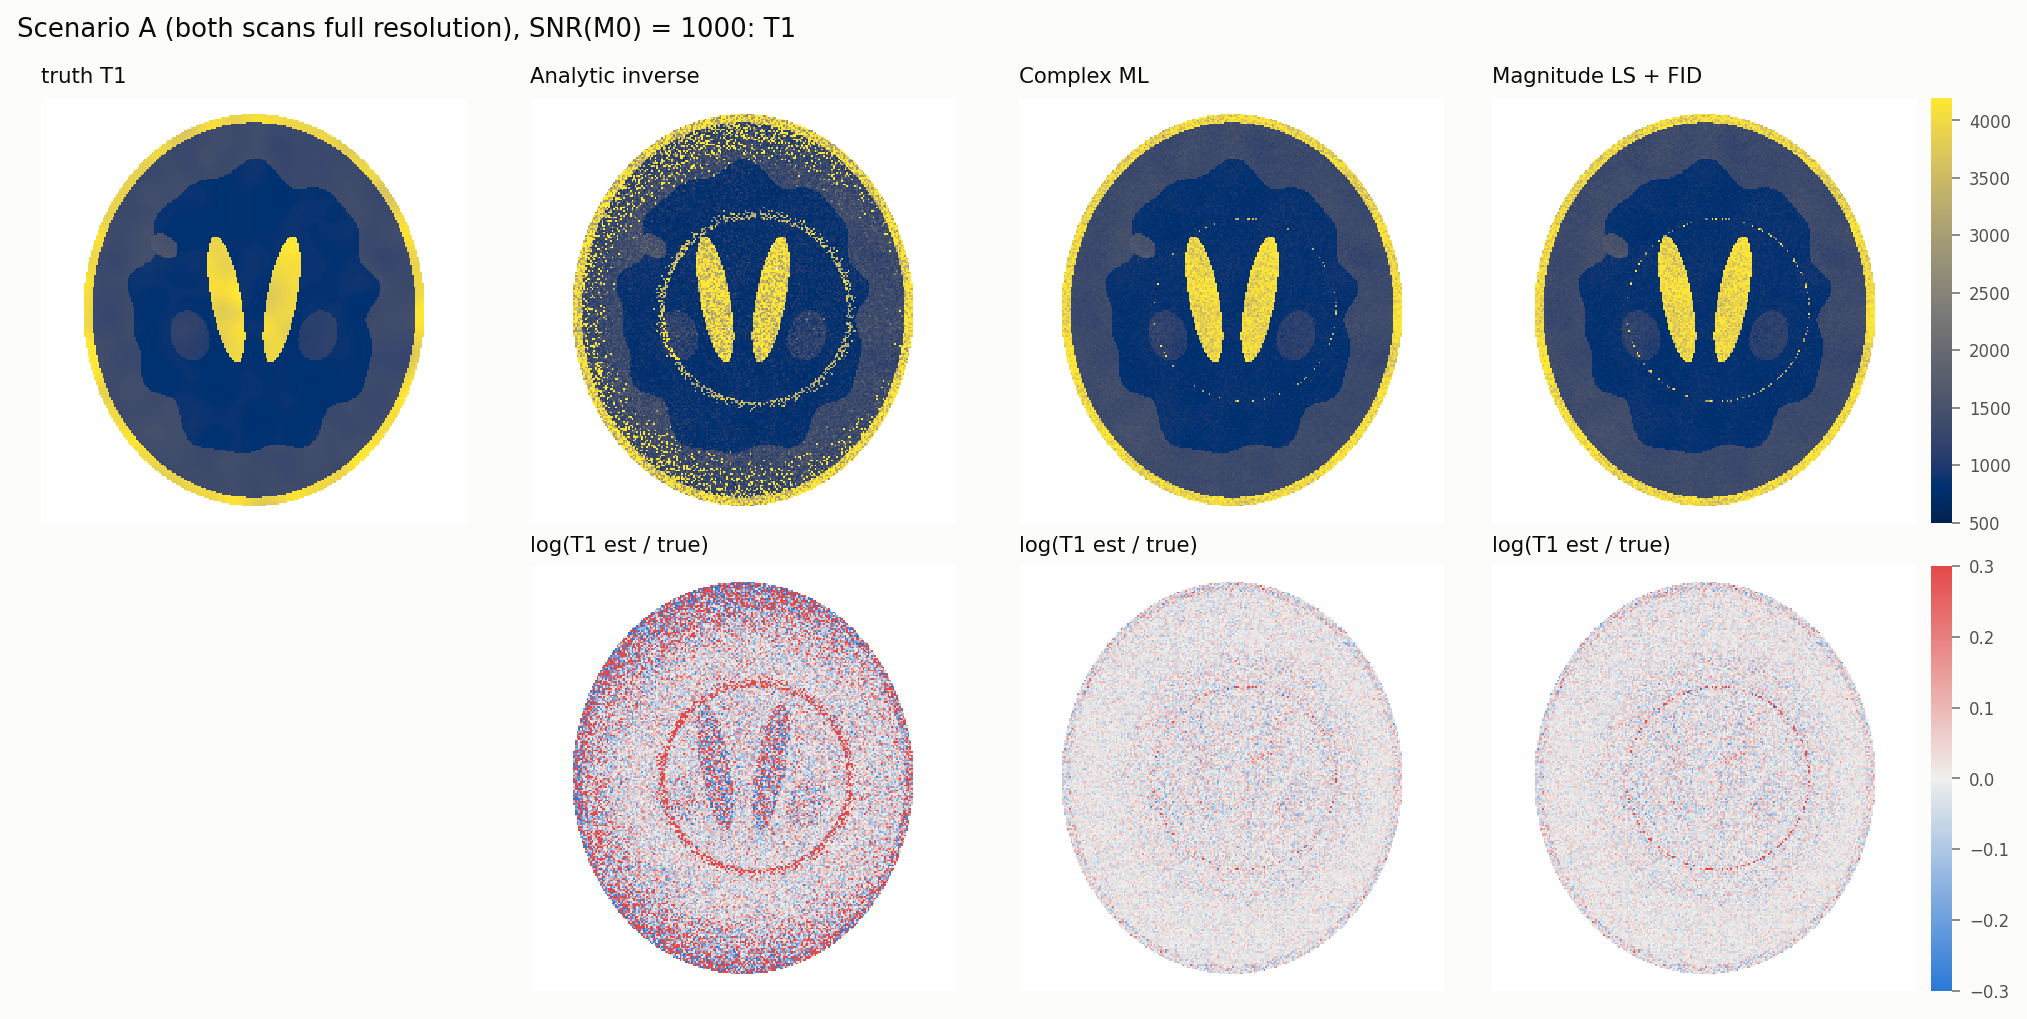
\includegraphics[width=\linewidth]{phantomA_T1_snr1000.png}
\caption{Scenario A, SNR$(\Mzero)=1000$: $\Tone$ maps and log-ratio error maps.}
\label{fig:phA_T1}
\end{figure}

\begin{figure}[!htbp]
\centering
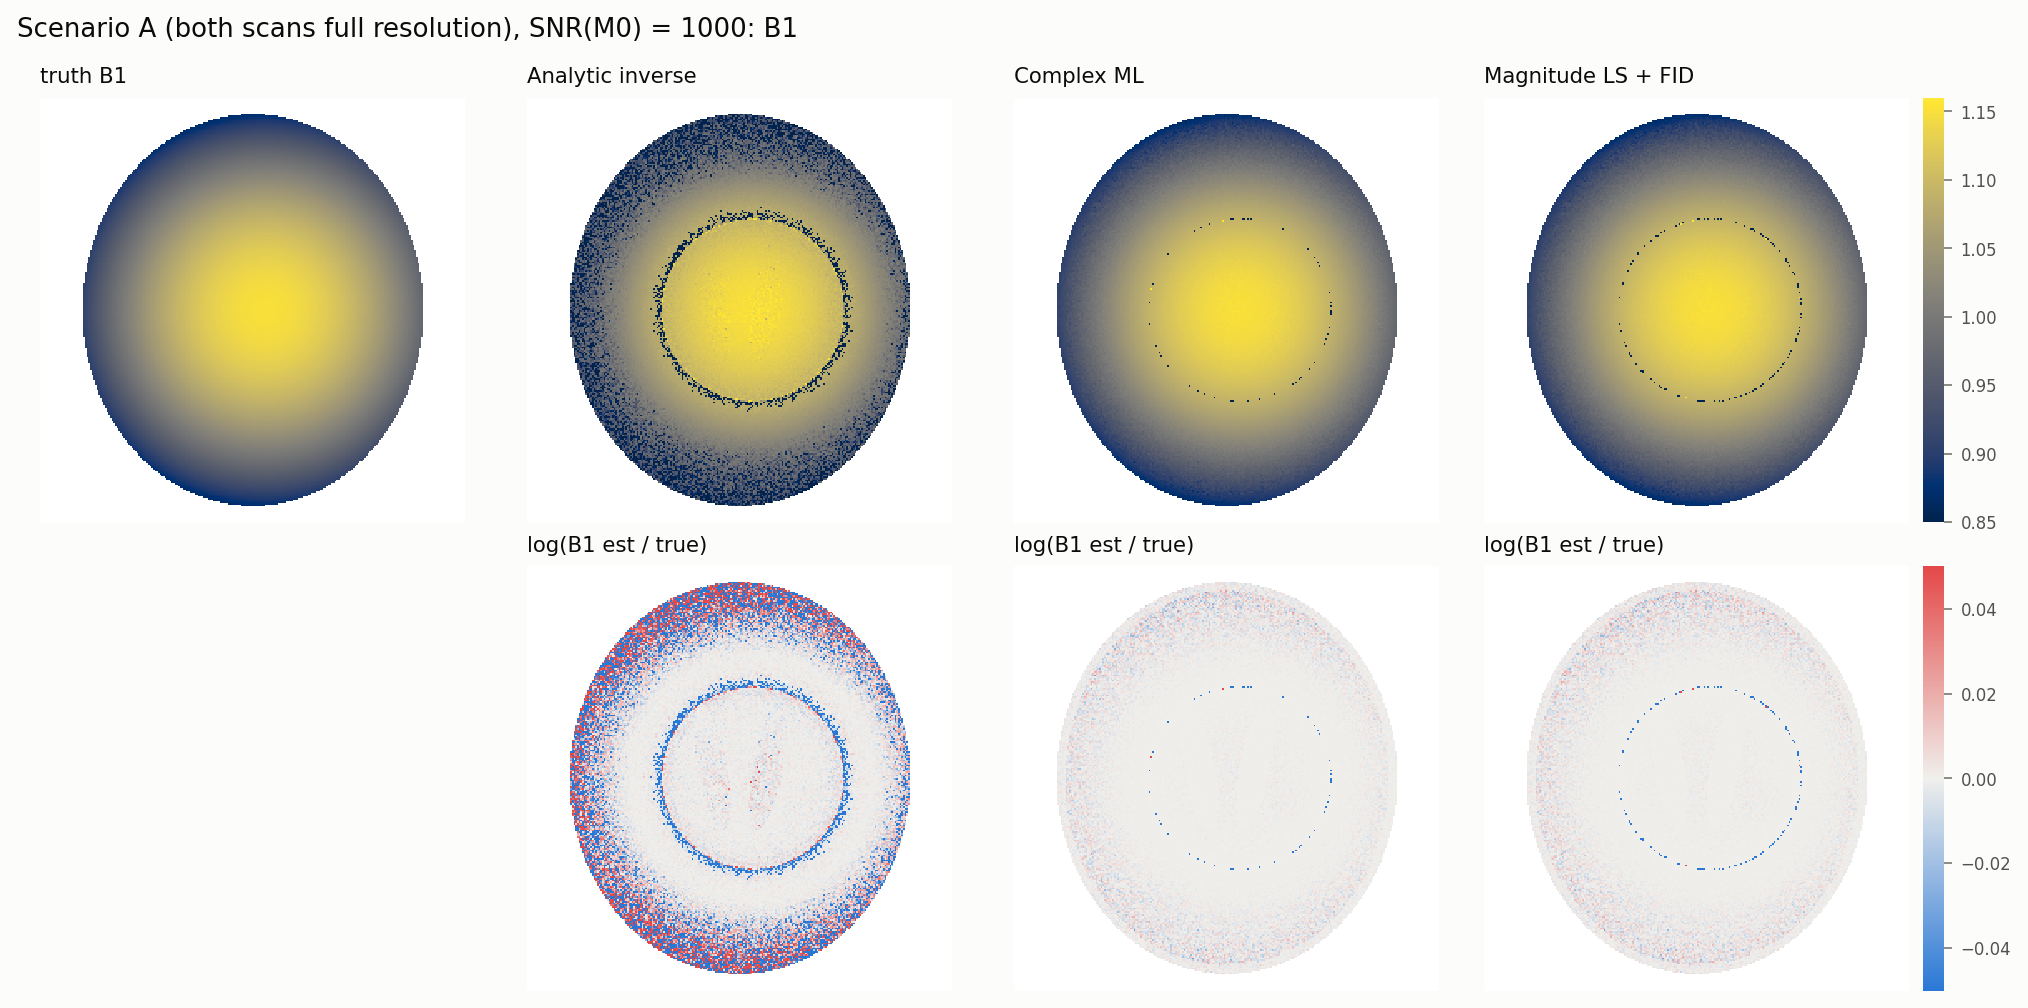
\includegraphics[width=\linewidth]{phantomA_B1_snr1000.png}
\caption{Scenario A, SNR$(\Mzero)=1000$: $\Bone$ maps and log-ratio error maps.}
\label{fig:phA_B1}
\end{figure}

\begin{figure}[!htbp]
\centering
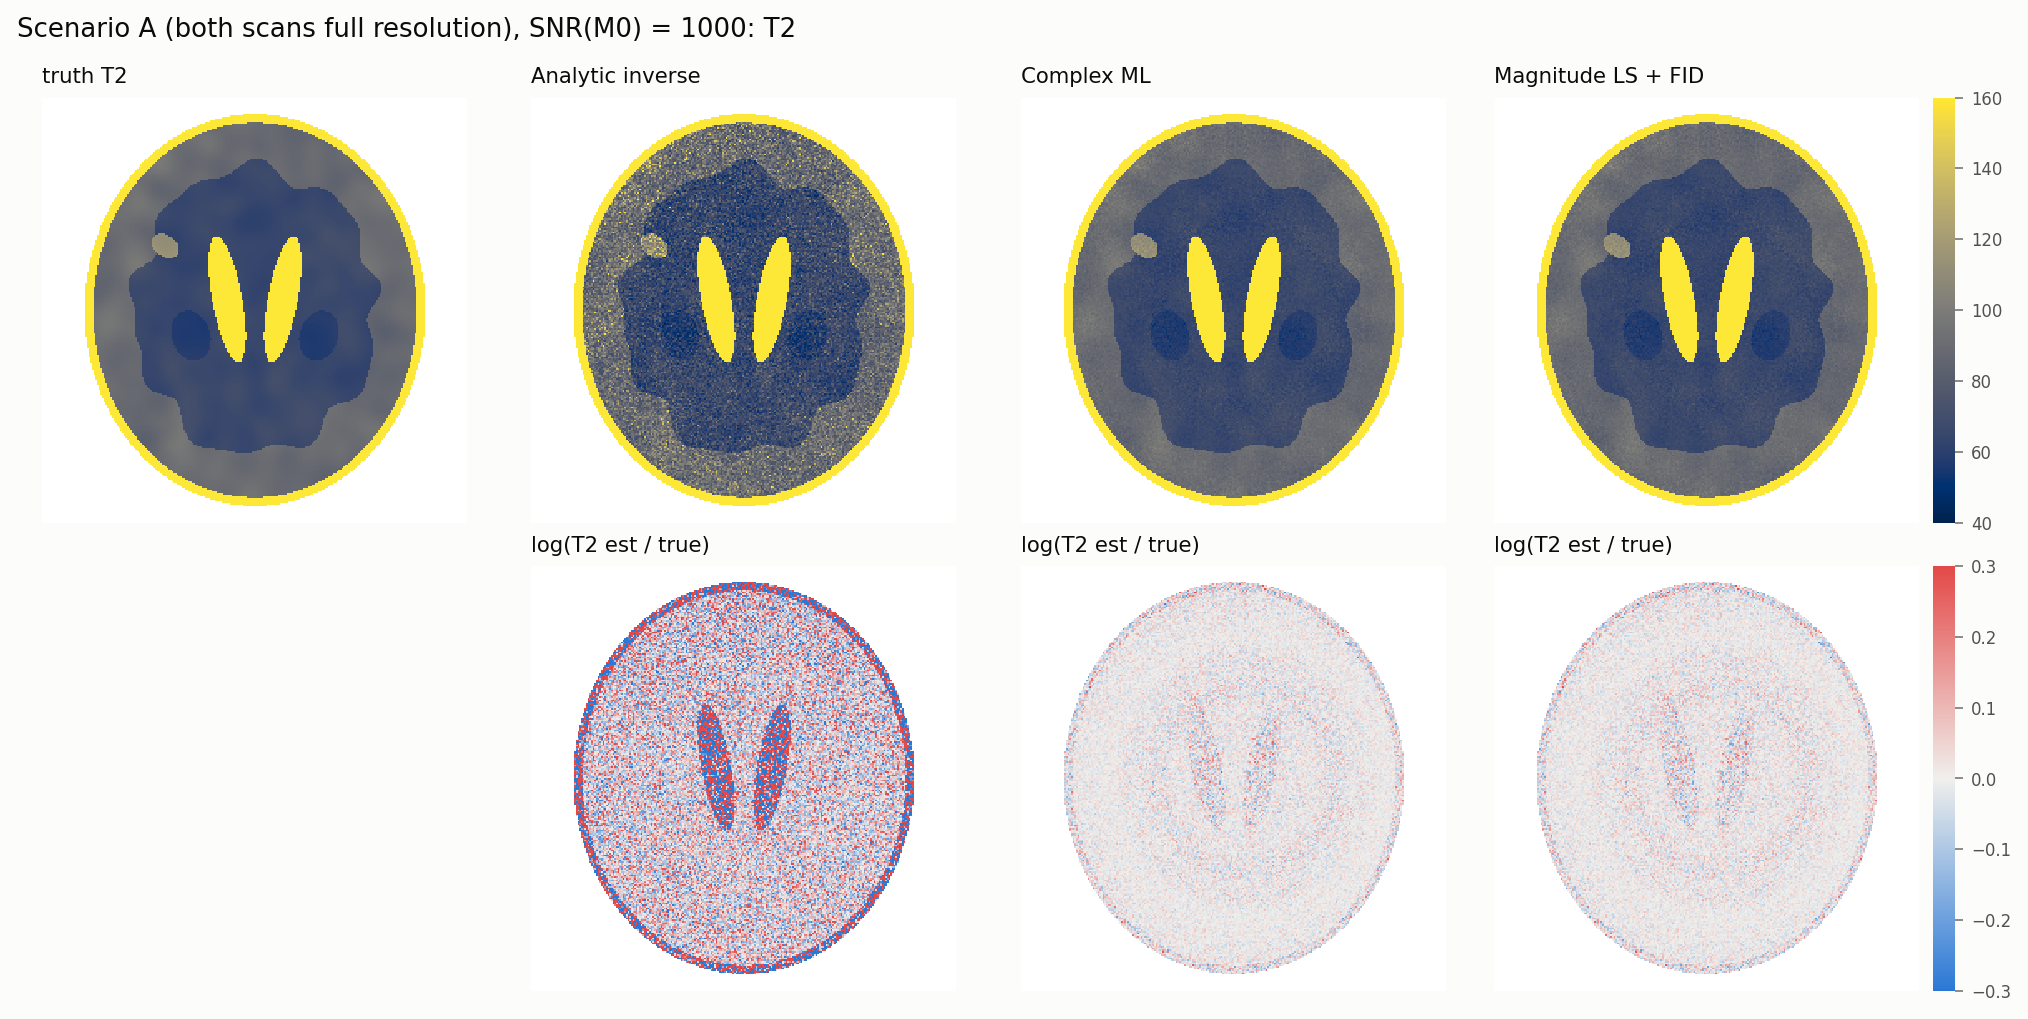
\includegraphics[width=\linewidth]{phantomA_T2_snr1000.png}
\caption{Scenario A, SNR$(\Mzero)=1000$: $\Ttwo$ maps and log-ratio error maps.}
\label{fig:phA_T2}
\end{figure}

\paragraph{Scenario A.} The maps reproduce the voxel-wise analysis
(\cref{fig:phA_T1,fig:phA_B1,fig:phA_T2}, \cref{tab:roi1000}). The analytic inverse is
unbiased in the median but noisy: at SNR 1000 its $\Tone$ spread is $0.30$ in white matter and
$0.40$ in grey matter, against $0.042$ for complex ML in grey matter, and its errors grow
towards the periphery (lower $\Bone$) and form a sharp ring at $\alpha_2=360^\circ$. Complex ML and
magnitude least squares with the FID sign are nearly indistinguishable, with negligible bias
in every tissue; their white-matter spread ($0.094$ and $0.124$) is inflated by the genuine
outliers on the $360^\circ$ ring, which lies in white matter, while the grey-matter spread ($0.042$)
is close to the voxel-wise bound. No voxel farther than $3^\circ$ from $360^\circ$ ends on the wrong branch
for any method.

\begin{figure}[!htbp]
\centering
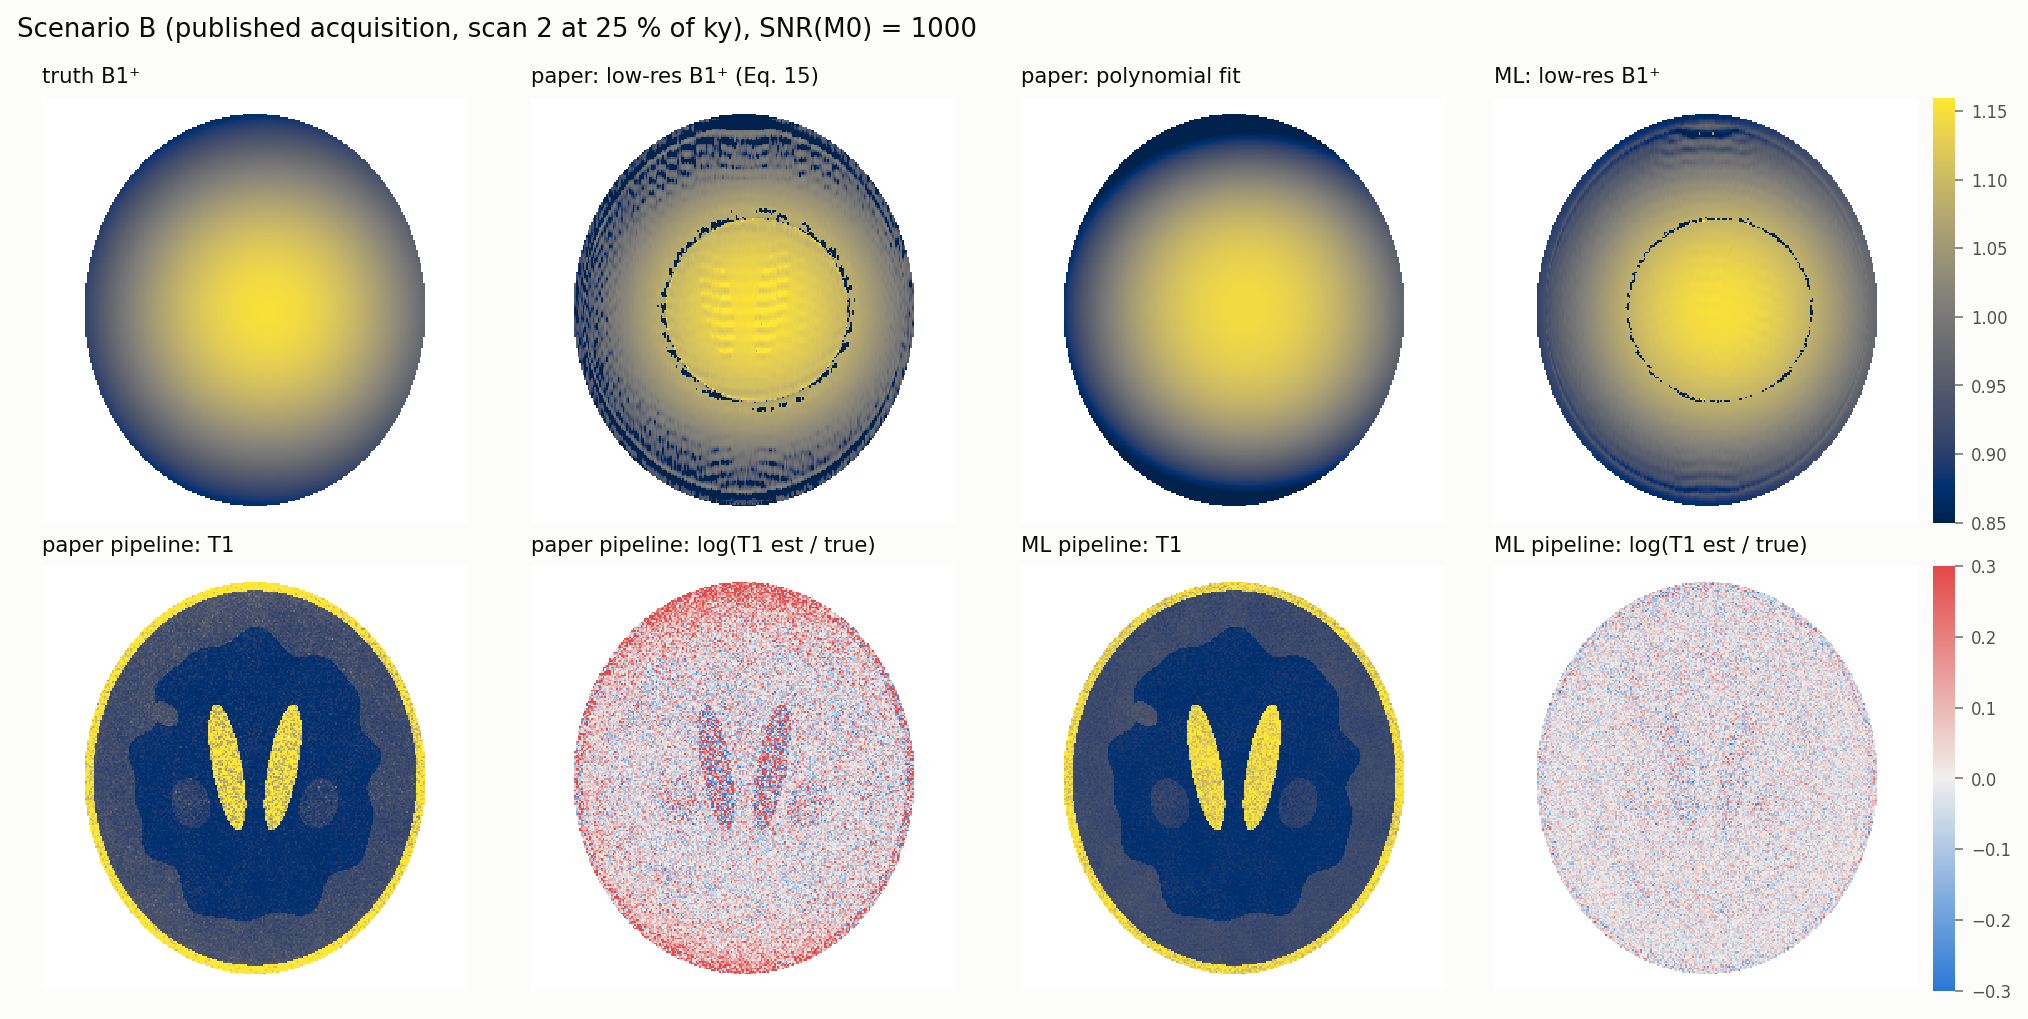
\includegraphics[width=\linewidth]{phantomB_snr1000.png}
\caption{Scenario B (scan 2 at $25\%$ of $k_y$), SNR$(\Mzero)=1000$. Top: true $\Bone$; low-resolution
$\Bone$ from Eq.~15; its polynomial fit; low-resolution $\Bone$ from complex ML. Bottom: $\Tone$ and its error
for the two pipelines.}
\label{fig:phB}
\end{figure}

\paragraph{Scenario B.} The low-resolution flip-angle map of the paper pipeline shows
truncation ringing, errors at the $360^\circ$ ring and outliers at the periphery
(\cref{fig:phB}); the polynomial fit absorbs much of this but remains biased by $-1.5\%$ in grey
matter (up to $15\%$ at the edge). Through the error transfer $\partial\log\Tone/\partial\log\Bone\approx-2$ of the
scan-1 $\Tone$ step (\cref{tab:cond}) this produces a $\Tone$ bias of $+4.3\%$ in grey matter and
$+8.5\%$ in CSF; with the true $\Bone$, the same $\Tone$ step is unbiased ($-0.06\%$ in grey matter). The
ML pipeline's smoothed map is accurate to $0.2\%$ everywhere and its $\Tone$ is unbiased in every
tissue. Its $\Tone$ spread is larger than in Scenario A in grey matter ($0.065$ vs $0.042$), as
expected from the scan-1-only bound ($57.1$ vs $40.5$), but smaller in white matter ($0.073$ vs
$0.094$), because a smooth, fixed $\Bone$ removes the $360^\circ$ ambiguity. Its $\Ttwo$ spread is larger than
in Scenario A because stage 2 uses only scan 1.

\paragraph{SNR 300.} \Cref{tab:roi300} gives the same statistics at SNR$(\Mzero)=300$
(image SNR about 26). The analytic inverse breaks down: its $\Tone$ spread is
$0.65$ in white matter and $0.91$ in grey matter, and $\Tone$ is undefined in $1.3$--$1.7\%$ of tissue
voxels and $17.8\%$ of CSF voxels. Complex ML and magnitude least squares with the FID sign
remain nearly unbiased, with spreads of $0.14$ (grey matter) to $0.28$ (CSF), no undefined
estimates and no wrong-branch voxels away from the $360^\circ$ ring (\cref{fig:phA_T1_300}). In
Scenario B the paper pipeline has spreads of $0.45$--$0.51$ in tissue and the same undefined
fractions, whereas the ML pipeline is nearly unbiased with spreads of $0.21$--$0.23$; its
grey-matter spread is $1.5$ times that of Scenario A, close to the bound ratio $57.1/40.5=1.4$.
At this SNR, errors above $0.3$ in log units are expected from noise alone in long-$\Tone$ tissue
(the local bound for CSF is of that order), and only 4 of \Voxels{} complex-ML voxels end above
the true-parameter cost.

\begin{figure}[!htbp]
\centering
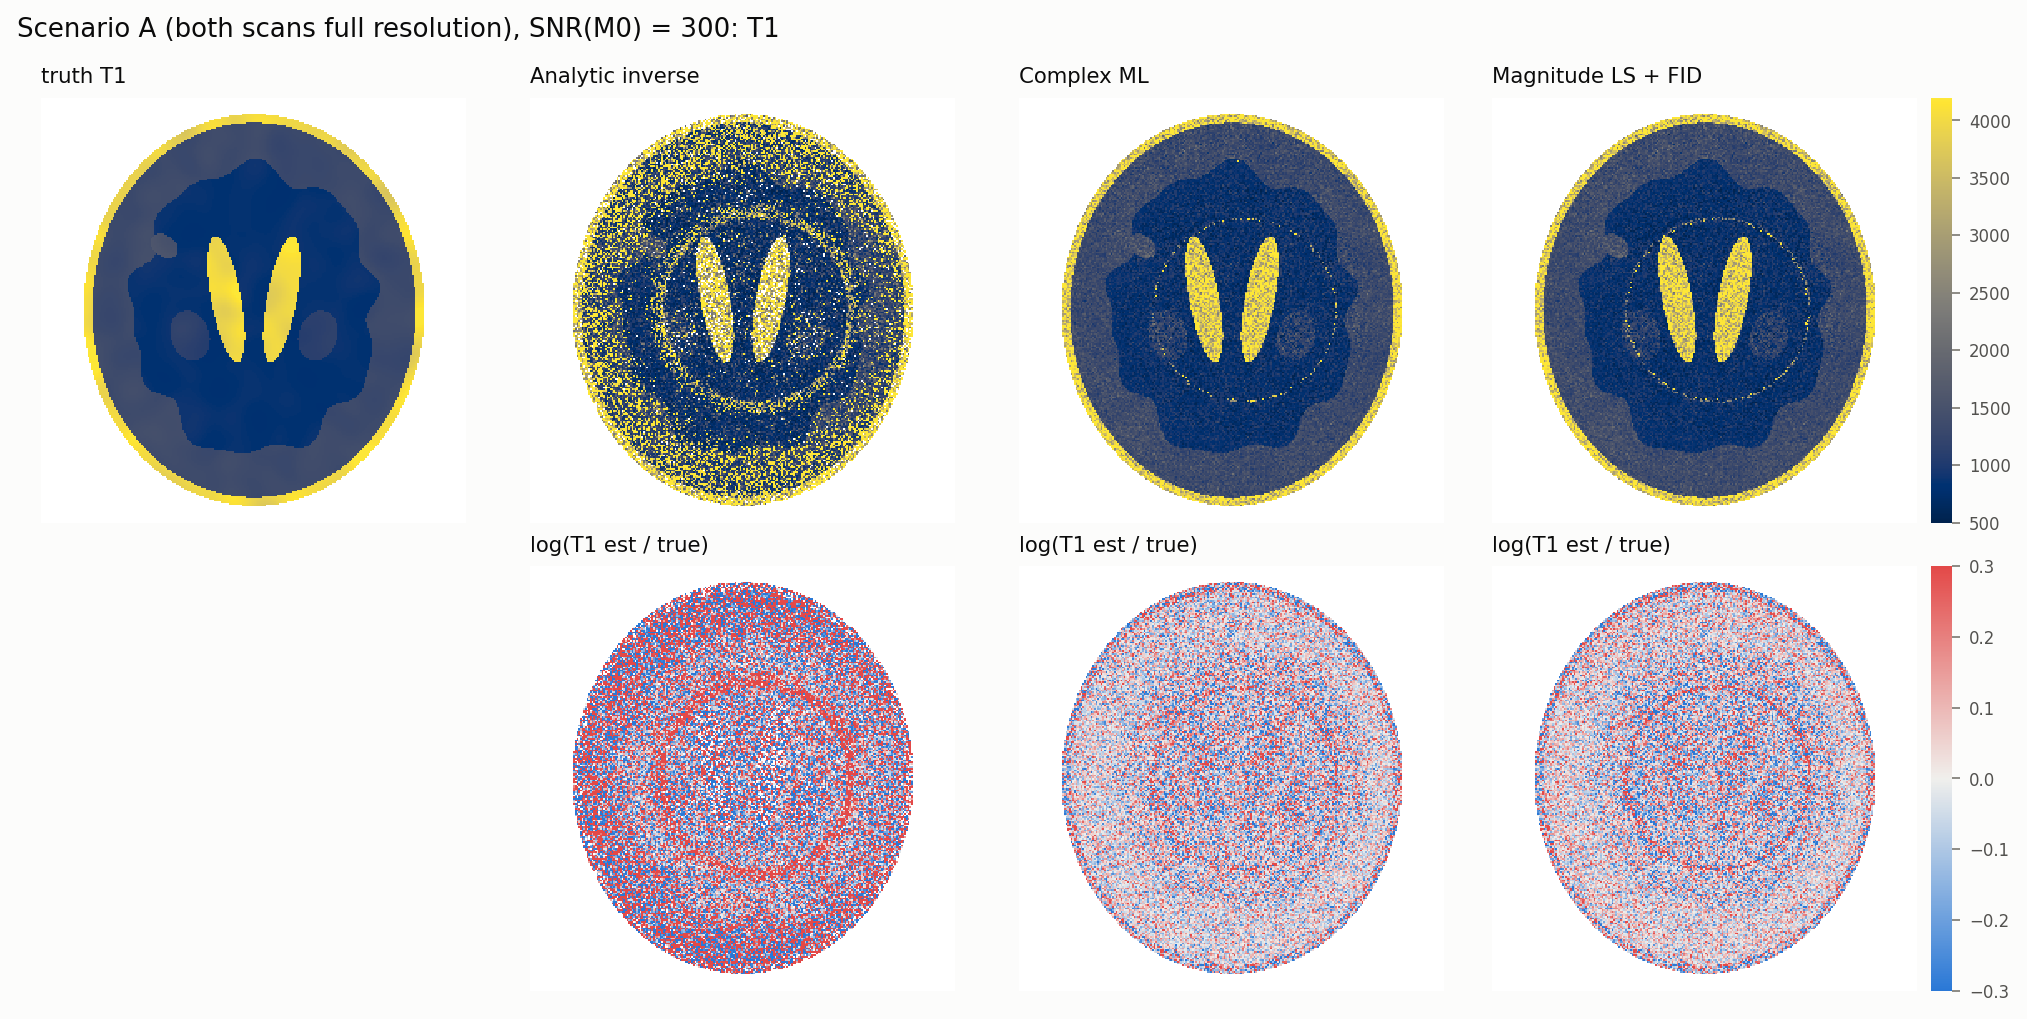
\includegraphics[width=\linewidth]{phantomA_T1_snr300.png}
\caption{Scenario A, SNR$(\Mzero)=300$: $\Tone$ maps and log-ratio error maps.}
\label{fig:phA_T1_300}
\end{figure}

\subsection{Uncertainty maps}

\begin{figure}[!htbp]
\centering
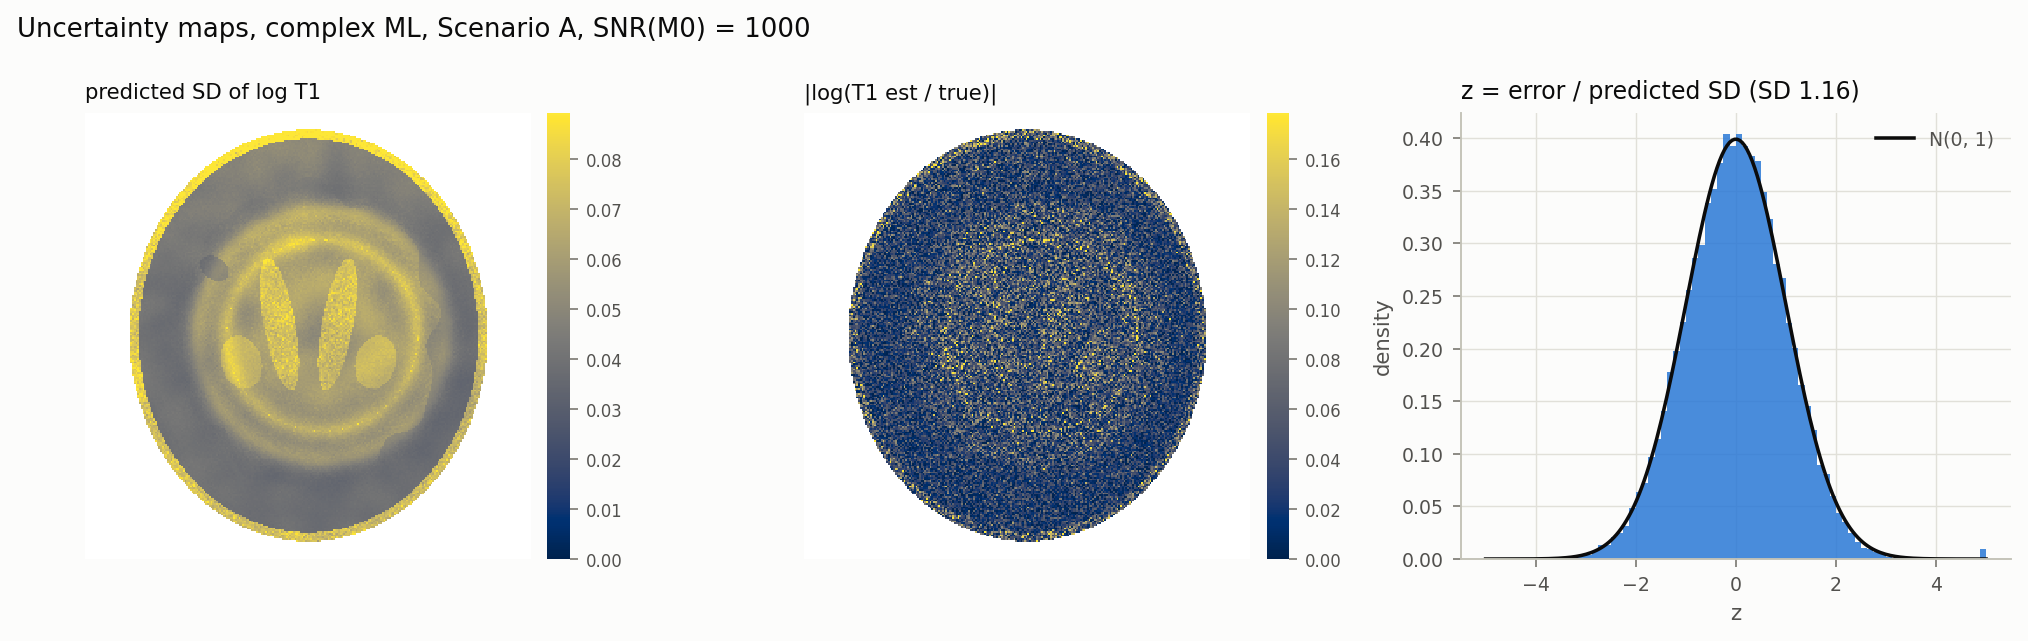
\includegraphics[width=\linewidth]{phantom_uncertainty_snr1000.png}
\caption{Complex ML, Scenario A, SNR$(\Mzero)=1000$: predicted SD of $\log\Tone$ (local CRLB at the
estimate), absolute error, and the distribution of the standardised error $z$ against $N(0,1)$
($z$ clipped to $\pm5$ for display).}
\label{fig:phunc}
\end{figure}

The local CRLB evaluated at the estimate gives a predicted standard deviation for every voxel
at the cost of one Jacobian (\cref{fig:phunc}). The map shows the structure expected from
\cref{sec:information}: higher uncertainty in CSF and long-$\Tone$ tissue, in deep grey matter, at
low $\Bone$, and on the $360^\circ$ ring. Standardised errors are close to $N(0,1)$. For complex ML in
Scenario A, $95\%$ intervals cover the truth in \CalAcovTThousand\% of voxels at SNR 1000
(\CalAcovTThreeHundred\% at SNR 300); the SD of $z$ is \CalAzTThousand{} (\CalAzTThreeHundred),
above 1 only because of the genuine outliers at $360^\circ$, which a local bound cannot describe.
For the ML pipeline of Scenario B (with $\Bone$ treated as known), coverage is
\CalBcovTThousand\% and \CalBcovTThreeHundred\% and the SD of $z$ is \CalBzTThousand{} and
\CalBzTThreeHundred{}: slightly conservative at SNR 300, consistent with the constraint
$\Rtwop\ge0$ being active in many voxels at that SNR (a constrained estimator can have a variance
below the interior bound, \cref{sec:ml}).

\subsection{Run times}

\begin{table}[!htbp]
\centering
\caption{Reconstruction times for the phantom (voxels in the mask; laptop CPU, 8 threads, implicit Jacobian, float64, 128 isochromats, 40 iterations).}
\label{tab:phantomtime}
\small
\begin{tabular}{lrr}
\toprule
Step & SNR 1000 & SNR 300\\
\midrule
A: analytic inverse & 3.0 s & 3.2 s\\
init (model fit) & 8.4 s & 9.1 s\\
A: complex ML (4 starts) & 131.0 s & 139.8 s\\
A: complex ML spatial restart & 34.1 s & 34.2 s\\
A: magnitude LS + FID sign (4 starts) & 120.9 s & 124.8 s\\
A: magnitude LS spatial restart & 30.2 s & 29.7 s\\
A: uncertainty maps & 2.6 s & 2.6 s\\
B: paper pipeline & 3.9 s & 4.2 s\\
B: ML pipeline & 194.8 s & 212.1 s\\
\bottomrule
\end{tabular}
\end{table}


A full set of reconstructions for one SNR level takes about 9 minutes on the laptop CPU
(\cref{tab:phantomtime}); each full-slice fit with four starts takes about 2 minutes, and the
uncertainty maps a few seconds.

\section{Partial volume: the BrainWeb phantom}\label{sec:pv}

The forward model assumes one tissue per voxel. Real voxels at 1--1.2\,mm often contain
several, and the cortex, two to three voxels thick, borders CSF almost everywhere. This
section measures the consequences with the BrainWeb anatomical model and the unchanged
estimators of \cref{sec:ml,sec:magnitude,sec:paper}, and explains them from the structure of
the model.

\subsection{The mixed-voxel signal}

If a voxel contains compartments $c$ with volume fractions $f_c$, proton densities $\mathrm{PD}_c$ and
relaxation parameters $\theta_c$, and shares the location-dependent quantities $\Bone$, $\dw$, $\phi_0$
and the receive sensitivity $C$, its signal is
\begin{equation}
  S^{\rm mix}_{ijk}=C\sum_cf_c\,\mathrm{PD}_c\;s_{ijk}(\theta_c),\qquad
  s_{ijk}(\theta_c)=v_{i,c}\,G_k(u_{i,c},E_{2,c},\dw)\,\E^{-t/T_{2,c}}\E^{-R'_{2,c}|t+k\TR|}\E^{i\Phi},
  \label{eq:mix}
\end{equation}
by \cref{thm:uv} applied to each compartment. A single-compartment estimator returns the
$\hat\theta$ whose model $S(\hat\theta)$ is closest to $S^{\rm mix}$ (in the sense of its own cost function).
Two questions follow: how far $S^{\rm mix}$ lies from the set of single-compartment signals (the
model manifold), which determines bias and detectability, and where on the manifold the
closest point lies, which determines the reported values.

\paragraph{Nearby compartments: a second-order effect.} If the compartments are close in
parameter space, write $\theta_c=\bar\theta+\delta_c$ with $\bar\theta$ the weighted mean (weights
$w_c=f_c\mathrm{PD}_c/\sum f\mathrm{PD}$, in log coordinates). Then
\begin{equation}
  \frac{S^{\rm mix}}{C\sum f\mathrm{PD}}=\sum_cw_cS(\theta_c)
  =S(\bar\theta)+\tfrac12\sum_cw_c\,\delta_c^{\mathsf T}\nabla^2S(\bar\theta)\,\delta_c+O(|\delta|^3),
  \label{eq:mix2}
\end{equation}
because the first-order terms cancel ($\sum w_c\delta_c=0$). The mixture is a single-compartment
signal at the weighted mean, up to a second-order term whose size is set by the curvature of
the model and the spread of the compartments. White and grey matter are close
($\Tone$ 850 vs 1350\,ms, $\Ttwo$ 66 vs 90\,ms): a WM/GM mixture is fitted to within $0.01\sigma$ per
measurement at SNR 1000 and reported at the weighted mean (median deviation $-0.013$ in
$\log\Tone$, \cref{tab:bwclean}). Such voxels are harmless: they look like an intermediate tissue,
which is what they are.

\paragraph{CSF: a first-order mismatch.} CSF is far from tissue ($\Tone=4000$\,ms, $\Ttwo=1500$\,ms),
so \eqref{eq:mix2} does not apply, and its signal contribution is strongly pathway- and
scan-dependent. Per unit volume, CSF produces $1.4$--$1.7$ times the grey-matter signal in the
FID of scan 1, but $2.6$--$3.4$ times in the echo pathways of scan 1 and $6.5$--$7.8$ times in
pathway $+1$ of scan 2 (proton-density ratio $1.22$): long $\Ttwo$ preserves the higher-order
configuration states that the echo pathways sample, and the large second pulse feeds them. A
voxel with $10\%$ CSF by volume therefore takes about $13\%$ of its FID but up to about $46\%$ of
its scan-2, $k=+1$ signal from CSF. No single $(\Tone,\Ttwo,\Ttwos)$ reproduces this pattern: the mixture
lies off the manifold, the residual is first order in the CSF fraction, and the fitted values
depend on which measurements an estimator weights most.

\paragraph{Consequences.} (i) Apparent parameters are not any simple average: relative to the
PD-weighted mean they are biased in a direction and by an amount that depend on the
parameter and the estimator (\cref{fig:bwcurves,tab:bwclean}). (ii) Different estimators no
longer agree, because they project the same off-manifold point differently: complex ML
weights all 36 measurements, the analytic inverse estimates $\Ttwo$ from scan 1 alone and $\Bone$
from closed-form ratios. (iii) The shared $\Bone$ absorbs part of the mismatch: the two scans see
the CSF admixture differently, and an estimator that ties them by a common $\Bone$ may shift
$\Bone$ to reconcile them. (iv) The residual grows only linearly with the CSF fraction while the
noise is fixed, so detectability depends on SNR: the noise-free cost $\|r\|^2$ makes the
residual $\chi^2$ non-central with parameter $\lambda=\|r\|^2/\sigma^2$, which grows as SNR$^2$.
(v) Uncertainty maps describe noise, not model error, so their coverage must drop wherever
the bias is comparable to the noise.

\subsection{Phantom and protocol}

We use the BrainWeb normal-brain anatomical model~\cite{collins1998,kwan1999,cocosco1997}: fuzzy
tissue-membership volumes at 1\,mm isotropic resolution ($181\times217\times181$). An axial slice through
the lateral ventricles (index 95, Talairach $z=23$\,mm) is zero-padded to $256\times256$. Voxels whose
discrete label is CSF, grey or white matter are kept (\,18\,668 voxels\,); fat, skin and skull are
excluded, since fat would require a chemical-shift model. Each compartment takes the tissue
values of \cref{tab:tissues} with a $3\%$ smooth texture, and the fields $\Bone$, $\dw$, $C$, $\phi_0$ are
those of \cref{sec:phantom}, rescaled to the head. Signals follow \eqref{eq:mix}. Of the
brain voxels, 13\,258 are pure (one tissue $\ge95\%$), 2818 are WM/GM mixtures and 2592 contain
5--95\% CSF (\cref{fig:bwphantom}).

Three cases are reconstructed with the estimators unchanged (four starts plus the spatial
restart for the two least-squares fits): \emph{noise-free with partial volume} (model error
alone), \emph{SNR 1000 with partial volume}, and a \emph{control} at SNR 1000 in which each
voxel is assigned entirely to its dominant tissue (same anatomy, no partial volume). For a
mixed voxel we report errors against the PD-weighted geometric mean
$\theta_{\rm eff}=\exp(\sum_cw_c\log\theta_c)$, and show the dominant-tissue value alongside, since a mixed
voxel has no single true value.

\begin{figure}[!htbp]
\centering
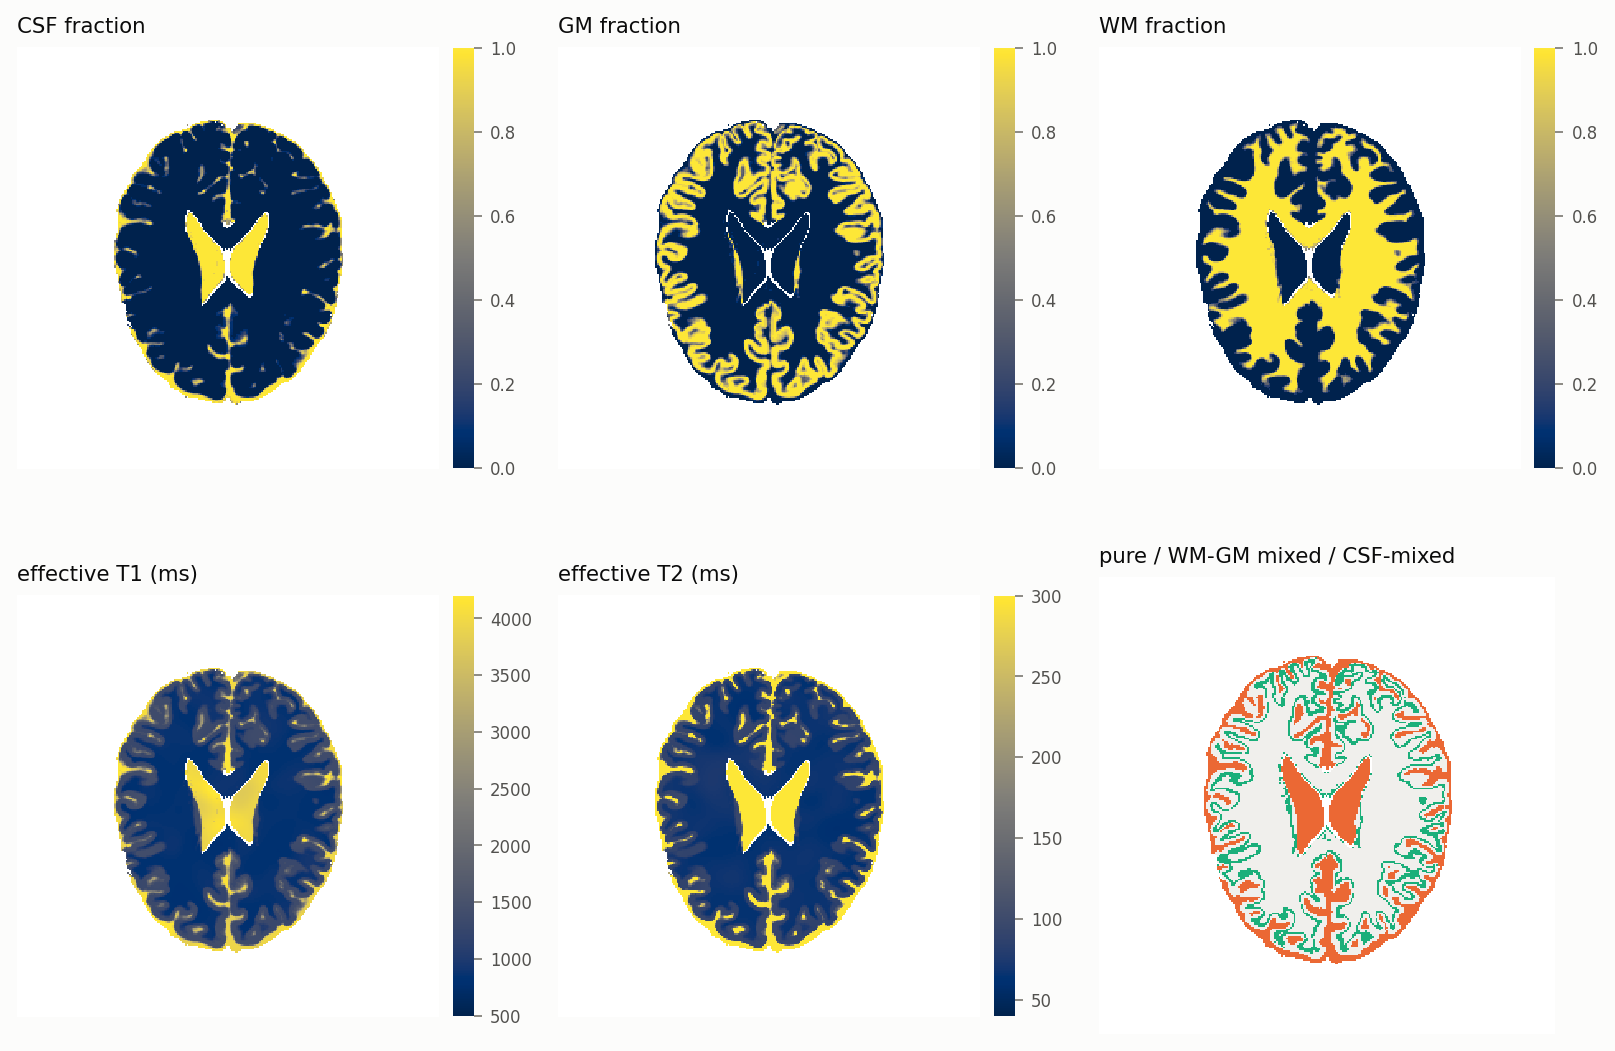
\includegraphics[width=0.92\linewidth]{brainweb_phantom.png}
\caption{BrainWeb slice: tissue fractions, the PD-weighted effective $\Tone$ and $\Ttwo$, and voxel
categories (pure; WM/GM mixed; containing $\ge5\%$ CSF).}
\label{fig:bwphantom}
\end{figure}

\subsection{Results}

\begin{table}[!htbp]
\centering
\caption{BrainWeb, noise-free: median of $\log(\hat\theta/\theta_{\rm eff})$ per voxel category, where $\theta_{\rm eff}$ is the PD-weighted geometric mean of the compartment values ($\Bone$: relative to the true field). Last columns: RMS mismatch residual per measurement in units of $\sigma$ at SNR 1000, and the probability that a $\chi^2$ test (99.9\,\%) flags the voxel at SNR 1000 and 3000.}
\label{tab:bwclean}
\footnotesize
\setlength{\tabcolsep}{3pt}
\begin{tabular}{lrcccccccc}
\toprule
 & & \multicolumn{3}{c}{Complex ML} & \multicolumn{3}{c}{Analytic inverse} & & \\
\cmidrule(lr){3-5}\cmidrule(lr){6-8}
Category & voxels & $\Tone$ & $\Ttwo$ & $\Bone$ & $\Tone$ & $\Ttwo$ & $\Bone$ & RMS/$\sigma$ & flagged 1000 / 3000\\
\midrule
pure CSF & 1823 & +0.000 & +0.000 & +0.000 & +0.000 & +0.000 & +0.000 & 0.00 & 0.1\,\% / 0.1\,\%\\
pure GM & 3931 & +0.000 & +0.000 & +0.000 & +0.000 & +0.000 & +0.000 & 0.00 & 0.1\,\% / 0.1\,\%\\
pure WM & 7504 & +0.000 & +0.000 & +0.000 & +0.000 & +0.000 & +0.000 & 0.00 & 0.1\,\% / 0.1\,\%\\
WM/GM mixed & 2818 & -0.013 & -0.009 & +0.000 & -0.017 & -0.006 & +0.000 & 0.01 & 0.1\,\% / 0.1\,\%\\
CSF 5-25\% & 1069 & -0.133 & -0.038 & +0.005 & -0.042 & -0.142 & -0.007 & 0.35 & 3.4\,\% / 59.2\,\%\\
CSF 25-50\% & 580 & -0.324 & -0.103 & +0.009 & -0.113 & -0.428 & -0.032 & 0.61 & 12.4\,\% / 95.7\,\%\\
CSF 50-95\% & 943 & -0.251 & -0.113 & +0.002 & -0.029 & -0.503 & -0.012 & 0.29 & 2.2\,\% / 48.1\,\%\\
\bottomrule
\end{tabular}
\end{table}

\begin{table}[!htbp]
\centering
\caption{BrainWeb at SNR$(\Mzero)=1000$, complex ML: SD of $\log(\hat\Tone/T_{1,\rm eff})$ with partial volume and in the control without it, coverage of $95\%$ uncertainty intervals, and the fraction of voxels flagged by the $\chi^2$ test.}
\label{tab:bwnoisy}
\footnotesize
\begin{tabular}{lccccc}
\toprule
Category & $\Tone$ SD (PV) & $\Tone$ SD (control) & median (PV) & coverage (PV) & flagged (PV)\\
\midrule
pure CSF & 0.077 & 0.077 & -0.003 & 94.7\,\% & 0.0\,\%\\
pure GM & 0.060 & 0.060 & +0.000 & 94.6\,\% & 0.2\,\%\\
pure WM & 0.084 & 0.084 & +0.000 & 94.9\,\% & 0.1\,\%\\
WM/GM mixed & 0.057 & 0.049 & -0.012 & 93.8\,\% & 0.1\,\%\\
CSF 5-25\% & 0.085 & 0.063 & -0.138 & 21.9\,\% & 4.0\,\%\\
CSF 25-50\% & 0.058 & 0.052 & -0.318 & 0.5\,\% & 15.2\,\%\\
CSF 50-95\% & 0.139 & 0.079 & -0.243 & 26.8\,\% & 3.1\,\%\\
\bottomrule
\end{tabular}
\end{table}


\begin{figure}[!htbp]
\centering
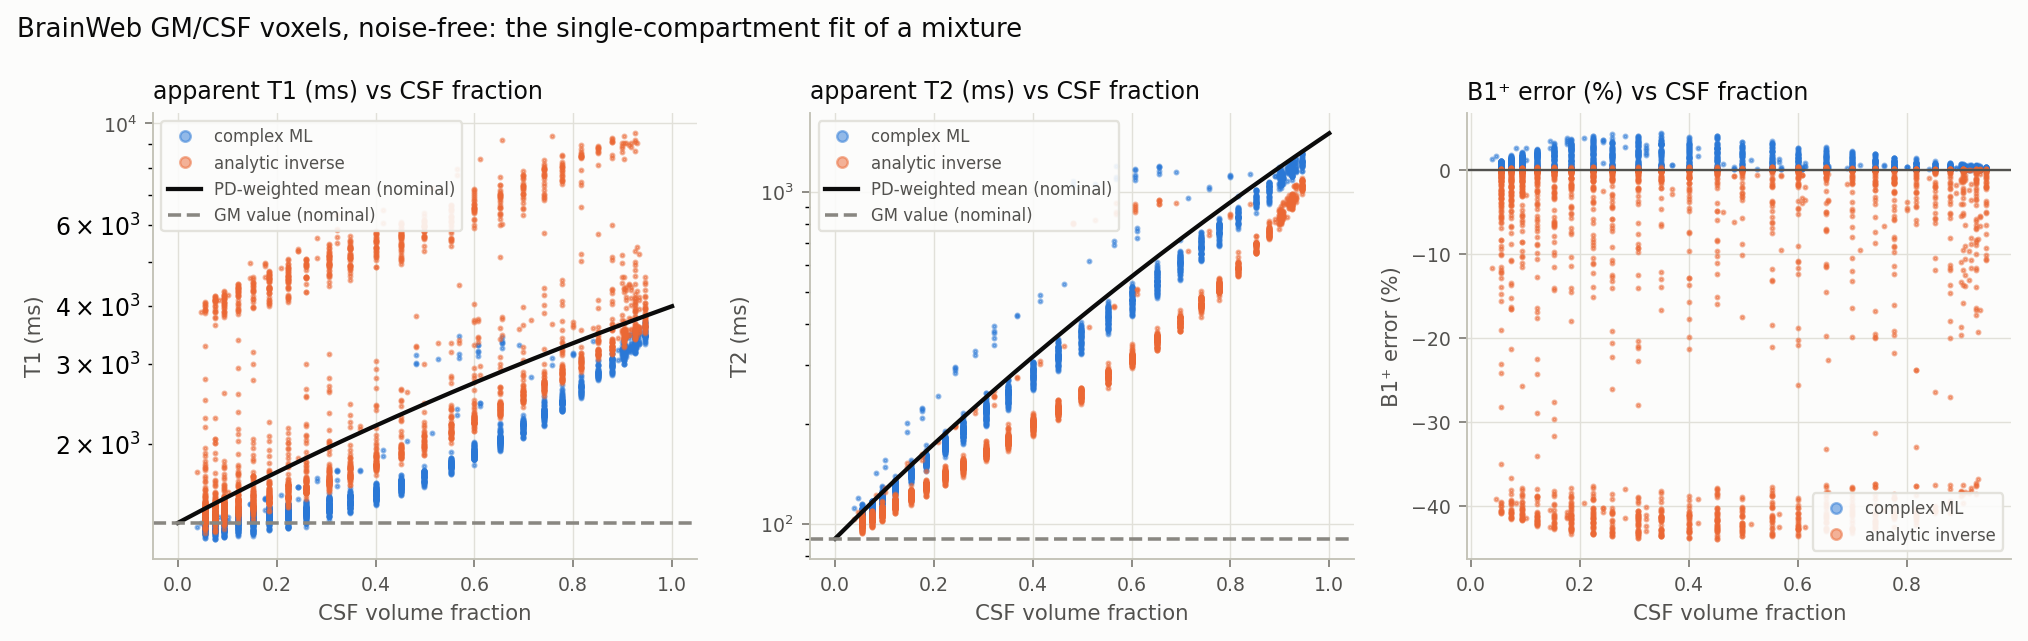
\includegraphics[width=\linewidth]{brainweb_mixture_curves.png}
\caption{Noise-free GM/CSF voxels ($<5\%$ WM): values returned by the single-compartment
estimators versus the CSF volume fraction, with the PD-weighted mean and the grey-matter value
(nominal, without texture). Right: $\Bone$ error.}
\label{fig:bwcurves}
\end{figure}

\begin{figure}[!htbp]
\centering
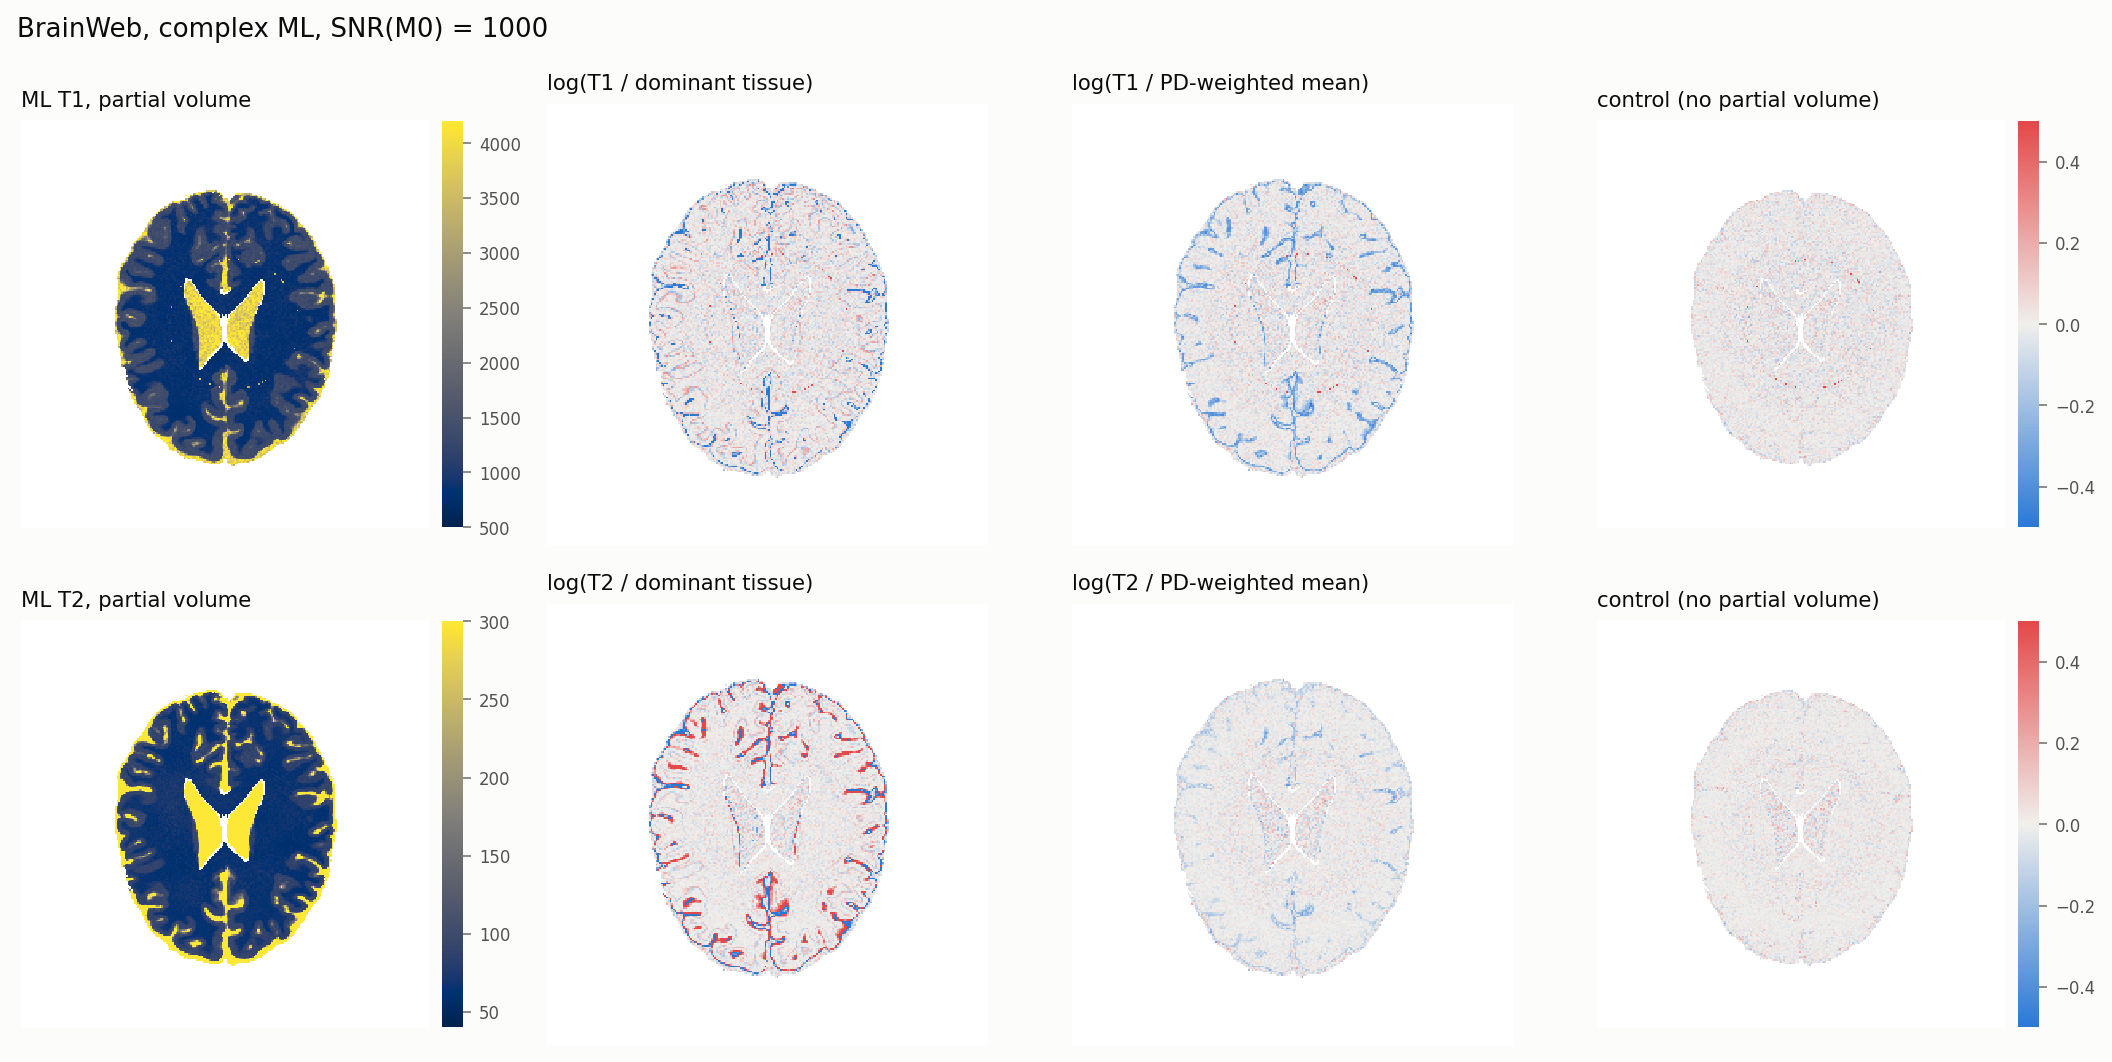
\includegraphics[width=\linewidth]{brainweb_maps.png}
\caption{Complex ML at SNR$(\Mzero)=1000$. From left: estimate with partial volume; log-ratio to the
dominant tissue's value; log-ratio to the PD-weighted mean; the same anatomy without partial
volume (control). Rows: $\Tone$ and $\Ttwo$.}
\label{fig:bwmaps}
\end{figure}

\paragraph{Pure tissue and WM/GM mixtures.} Pure voxels are reconstructed without bias by all
estimators, and complex ML has the same spread and $94.6$--$94.9\%$ coverage as in the control
(\cref{tab:bwnoisy}). WM/GM mixtures are fitted to $0.01\sigma$ per measurement, reported at the
PD-weighted mean to within $-0.013$ in $\log\Tone$ and $-0.009$ in $\log\Ttwo$ for complex ML, and their
coverage ($93.8\%$) is close to nominal: the second-order picture of \eqref{eq:mix2} holds.

\paragraph{CSF-mixed voxels: biased, confidently.} In the 2592 voxels with $5$--$95\%$ CSF all
estimators are biased by far more than the noise (\cref{tab:bwclean,fig:bwcurves,fig:bwmaps}).
For complex ML the deviation of $\log\Tone$ from the PD-weighted mean is $-0.13$, $-0.32$ and $-0.24$
in the three CSF bins; $\Ttwo$ deviates by $-0.04$ to $-0.11$ from the mean but lies far above the
grey-matter value (\cref{fig:bwcurves}: at $10\%$ CSF the apparent $\Ttwo$ is about $40\%$ above that of
grey matter). Against the dominant tissue, the cortex therefore appears with elevated $\Ttwo$ and,
where CSF dominates, depressed $\Tone$ (\cref{fig:bwmaps}). The noise spread in these voxels is
similar to the control (\cref{tab:bwnoisy}), so the uncertainty maps report small intervals
around a biased value: coverage of $95\%$ intervals drops to $21.9\%$, $0.5\%$ and $26.8\%$, against
$94$--$95.5\%$ in the control. The residual does not reveal the problem at this SNR: the mismatch
is $0.29$--$0.61\sigma$ per measurement, and a $\chi^2$ test at $99.9\%$ flags $3$--$15\%$ of these voxels at
SNR 1000 (predicted $2.2$--$12.4\%$ from the noise-free residual), rising to $48$--$96\%$ only at SNR
3000.

\paragraph{The estimators disagree.} Complex ML and magnitude least squares return the same
values (both fit all measurements), but the analytic inverse does not: its $\Ttwo$ deviates by
$-0.14$ to $-0.50$ from the mean (it uses scan 1 only), and in $19.5$--$38\%$ of the CSF-mixed voxels
the mismatch moves its flip-angle equation onto a different root, with $\Bone$ about $40\%$ too low
and $\Tone$ of $4$--$9$\,s even without noise (\cref{fig:bwcurves}, right). Complex ML's $\Bone$ stays within
$+4\%$ in every mixed voxel; its error is confined to the relaxation times.

\subsection{What partial volume does to the model and the estimators}

\begin{enumerate}
\item \textbf{Partial volume is a model error, not noise.} It biases every single-compartment
  estimator, does not average out with more data, and is invisible to the CRLB, which assumes
  the model is correct. Efficiency comparisons (\cref{sec:ml}) remain valid in pure voxels,
  where they were made.
\item \textbf{Its size is governed by distance on the model manifold.} Mixtures of nearby
  tissues are, to second order, single-compartment signals at the weighted mean \eqref{eq:mix2};
  they are harmless and should be read as intermediate tissue. Mixtures with CSF are far from the
  manifold because CSF's long $\Ttwo$ inflates its contribution to the echo pathways and to the
  second scan, up to eight times its volume share: the reported values then depend on the
  measurements an estimator weights most, and no estimator returns a well-defined average.
\item \textbf{It is hard to detect per voxel.} The mismatch residual grows linearly with the
  CSF fraction while the noise is fixed, so a $\chi^2$ test detects partial volume only at high SNR
  or after averaging. Per-voxel uncertainty maps become falsely confident where it acts; they
  should be reported together with a partial-volume indicator, e.g.\ the distance to a tissue
  boundary from a segmentation, or the fit of a mixture model.
\item \textbf{The shared $\Bone$ matters.} Because $\Bone$ couples the two scans, an estimator that uses the
  scans in separate closed-form steps (the analytic inverse) can resolve the mismatch by a large
  $\Bone$ error, whereas the joint fit keeps $\Bone$ nearly unbiased and pushes the error into the
  relaxation times. For the two-stage design this favours estimating $\Bone$ from robustly smoothed
  maps, which the polynomial fit already provides: partial-volume errors are local and are
  rejected as outliers.
\item \textbf{Remedy.} A two-compartment model,
  $S=C\,[f\,\mathrm{PD}_as(\theta_a)+(1-f)\,\mathrm{PD}_bs(\theta_b)]$ with shared $\Bone$, $\dw$, $\phi_0$, is the natural
  correction. Fitting both compartments freely is ill-conditioned (13 parameters, near-collinear
  signals), but with class parameters fixed from pure voxels or a population estimate (the
  hierarchical model of \cref{sec:future}) the signal is linear in the fractions given $\Bone$, $\dw$,
  $\phi_0$, and variable projection reduces the fit to a small nonlinear problem. CSF fractions should
  then be well determined, because CSF's signature is distinct, whereas WM/GM fractions will be
  poorly determined---and, by item 2, need not be. The implicit Jacobian, the CRLB machinery and
  the FID-sign test carry over unchanged (every compartment's FID has the sign of $\sin\alpha$).
\end{enumerate}

\section{Discussion}\label{sec:discussion}

\subsection{Forward model or inverse?}

\begin{table}[!htbp]
\centering
\caption{Origin of each difficulty.}
\label{tab:verdict}
\small
\begin{tabular}{p{0.38\linewidth}p{0.22\linewidth}p{0.32\linewidth}}
\toprule
Difficulty & Origin & Remedy\\
\midrule
One scan cannot separate $\Mzero,\Bone,\Tone$ (\cref{cor:onescan}) & forward model (exact) & two scans with a common $\Bone$\\
Small flip angles: leading-order invariance \eqref{eq:sym}, severe ill-conditioning & forward model $+$ protocol & a pulse whose effective angle does not scale with $\Bone$ (near $360^\circ$, as published)\\
Residual $\Tone$ bound ($40.5\,\sigma/\Mzero$): confounding with $\Ttwo$, $\Ttwos$, $\Mzero$, $\Bone$ & forward model $+$ protocol & SNR, averaging, spatial priors; protocol tuning ($\le20\%$ for flip angles)\\
Exact magnitude alias $\alpha_2=360^\circ\mp x$ at physiological $\Bone$ & forward model: magnitudes lose $\sgn\sin\alpha$ & FID-sign test, or complex data with a shared phase\\
Exact complex alias $\alpha_2>540^\circ$ & forward model: $2\pi$ periodicity & range bound $\Bone<1.64$\\
Error 3--7$\times$ the bound; bias and undefined $\Tone$ at moderate SNR & analytic inverse (sequential, closed form) & joint ML or magnitude least squares with the FID sign\\
$\Tone$ bound 57.1 instead of 28.0 with $\Bone$ known; $\Tone$ bias $-2\varepsilon$ per $\Bone$ error $\varepsilon$ & design: scan-1-only $\Tone$ step, low-resolution scan 2 & joint estimation; full-resolution scan 2 if affordable\\
Estimates on $\Rtwop=0$ at low SNR & model domain $+$ small true $\Rtwop$ & report; Bayesian or constrained bounds\\
One start insufficient & nonconvex likelihood & multiple starts (affordable with exact Jacobians)\\
In-vivo calibration $\beta=1.24$ & model mismatch (not variance) & richer forward model (\cref{sec:future})\\
\bottomrule
\end{tabular}
\end{table}

The published protocol is sound from an information standpoint: the near-$360^\circ$ pulse lifts
the leading-order invariance that makes $\Bone$/$\Tone$ separation hopeless with small angles, and the
data contain the information that the bounds promise. The published inverse does not extract
it efficiently; joint estimation does, for complex data and, with one bit of phase, for
magnitudes. The phantom (\cref{sec:phantom}) confirms these conclusions spatially and
quantifies the cost of the low-resolution second scan.

No unbiased voxel-wise estimator can beat the bounds of \cref{sec:information}. Further gains
require prior information: $\Bone$ is spatially smooth and can be treated as nearly known (removing
its factor of about $1.45$), while the confounding with $\Mzero$ and the transverse relaxation times
can only be reduced by priors on the parameter maps themselves. Such estimators are biased by
design, and their bias must be measured rather than ignored.

\subsection{Limitations}

The forward model assumes instantaneous RF pulses, a Lorentzian intravoxel frequency
distribution, no diffusion, no magnetisation transfer, no flow or motion, a single
compartment per voxel, and perfect steady state; the time from the pulse to the first echo
is assumed (4.5\,ms). The CRLB is local and assumes an exact model, Gaussian noise, an interior
true parameter and locally unbiased estimators. The digital phantom is noise-only and
model-consistent: it validates estimators and uncertainty maps but not the model itself.

\subsection{Future work}\label{sec:future}

\paragraph{Model mismatch.} The in-vivo calibration $\beta=1.24$ of~\cite{cheng2019}, unexplained by
the authors and absent in phantoms, indicates that the forward model misses something in
vivo. Candidates, each of which can be added to the simulator and assessed by fitting
mismatched data with the current model: (i) finite hard pulses with off-resonance during the
pulse (their Eq.~8 nutation function) and an inaccurate ratio of the actual flip angles; (ii)
non-Lorentzian intravoxel frequency distributions (e.g.\ Gaussian or susceptibility-driven),
which change $\exp(-\Rtwop|\tau|)$; (iii) diffusion attenuation of the higher-order pathways
under the unbalanced gradient (already available in the EPG simulator); (iv) magnetisation
transfer, which lowers the effective longitudinal magnetisation under the large pulse; (v)
partial volume (two compartments per voxel); (vi) $B_0$ drift or motion between the sequential
scans, which corrupts the relative phase used by the branch test and by complex ML. The
measure of interest is the bias each effect induces in $\Tone$ and $\Bone$ relative to the noise
spread, and whether a single global factor like $\beta$ can absorb it.

\paragraph{Rician maximum likelihood.} Magnitude least squares ignores the Rician noise floor.
At the published protocol the induced bias is small (\cref{sec:magnitude}), but it grows with
lower SNR, smaller flip angles or protocols with weaker pathways. Two routes are natural.
(i) Direct ML with the Rician likelihood
$\log p(m\mid A)=\log m-\log\sigma^2-(m^2+A^2)/(2\sigma^2)+\log I_0(mA/\sigma^2)$, whose gradient and
Gauss--Newton approximation follow from the exact Jacobian of $A=|s(\theta)|$. (ii) An EM algorithm
that treats the lost phase as missing data: with $\kappa=m|s_t|/\sigma^2$, the E-step gives
$\mathbb E[|z|\mid m]=m\,I_1(\kappa)/I_0(\kappa)$ and the M-step is magnitude least squares on these
shrunk pseudo-data, which is the existing fit. Either should be combined with the FID-sign
constraint, which the alias of \cref{prop:equiv} requires for any magnitude likelihood.
The Rician Fisher information of \cref{sec:rician} provides the reference bound.

\paragraph{Hierarchical (empirical-Bayes) estimation.} A hierarchical model with tissue classes
(a Gaussian mixture in $(\log\Tone,\log\Ttwo,\log\Ttwos)$) and a smooth parametric $\Bone$ field, whose
hyperparameters are estimated by EM with a Laplace E-step (MAP fit plus
$(J^{\mathsf T}J+\Sigma_k^{-1})^{-1}$ per voxel and class), would use the subject's own data as the
prior. It targets exactly the weak direction of \cref{fig:eigen} and makes the $\Bone$ field
effectively known; its bias would be evaluated on the phantom, including the lesion.

\paragraph{Learned estimators.} Networks trained on simulated signals~\cite{cheng2020} are
biased estimators whose prior is the training distribution. The tools here---exact bounds,
efficient ML as a reference, calibrated uncertainty, and the phantom---are what is needed to
measure their bias and variance against the CRLB rather than only their average error.

\paragraph{Acquisition.} Direct CRLB-based optimisation of $\TR$, flip angles, echo placement
and scan-2 coverage, now cheap (\cref{sec:jacobian}); and the joint use of a low-resolution
scan 2 inside a single likelihood (modelling its $k$-space truncation) instead of the two-stage
pipeline.


\appendix
\section{Proofs and derivations}\label{app:proofs}

The proofs of \cref{prop:offres}, \cref{thm:uv}, \cref{lem:absv}, \cref{cor:onescan},
\cref{prop:paperconsistent}, \cref{prop:scaling}, \cref{prop:period} and \cref{prop:equiv} are
given in the main text. This appendix contains the remaining derivations.

\subsection{Direct small-angle expansion of the isochromat solution}\label{app:scaling}

This gives the leading term of \cref{prop:scaling} in explicit form, independently of
\cref{thm:uv}. Use the notation of the proof of \cref{thm:uv} with $\varphi=\dw=0$, write
$m_\perp$ and $m_z$ for the post-pulse state, $m_\perp^-=E_2\E^{i\psi}m_\perp$ and
$Z=m_z^-=E_1m_z+1-E_1$ for the pre-pulse state. The pulse gives
\[
  m_\perp=m_\perp^--i\sin\alpha\,Z+i(\cos\alpha-1)\Im m_\perp^-,\qquad
  m_z=\sin\alpha\,\Im m_\perp^-+\cos\alpha\,Z .
\]
In the steady state $Z=O(1)$ and $m_\perp=O(\alpha)$, so the last term in $m_\perp$ is $O(\alpha^3)$ and
\begin{equation}
  m_\perp=\frac{-i\alpha Z}{1-E_2\E^{i\psi}}+O(\alpha^3),\qquad |1-E_2\E^{i\psi}|\ge1-E_2>0 .
\end{equation}
With $E_1=1-\rho+O(\rho^2)$, $m_z=Z-\rho(1-Z)+O(\rho^2)$, and with $\cos\alpha=1-\alpha^2/2+O(\alpha^4)$ the
longitudinal equation becomes
$\rho(1-Z)=-\alpha\Im m_\perp^-+\tfrac{\alpha^2}{2}Z+O(\alpha^4+\rho^2+\alpha^2\rho)$. From the transverse result,
$\Im m_\perp^-=-\alpha Z(E_2\cos\psi-E_2^2)/|1-E_2\E^{i\psi}|^2$, and
\[
  \frac{E_2\cos\psi-E_2^2}{|1-E_2\E^{i\psi}|^2}+\frac12=\frac12H(\psi),\qquad
  H(\psi)=\frac{1-E_2^2}{1-2E_2\cos\psi+E_2^2}.
\]
Hence $Z=[1+cH(\psi)]^{-1}$ with $c=\alpha^2/(2\rho)$ to leading order, and
\begin{equation}
  m_\perp(\psi)=\frac{-i\alpha}{(1-E_2\E^{i\psi})\,[1+cH(\psi)]}+O(\alpha^3+\alpha\rho),
\end{equation}
uniformly in $\psi$ because $1+cH\ge1$. Its Fourier coefficients are $\alpha f_k(c,E_2)$ plus a
remainder bounded by the uniform remainder, which proves \eqref{eq:scaling} for every $k$.
(Consistency with \cref{prop:scaling}: $u\to(c-1)/(c+1)$ and $v\to\alpha/(1+c)$.)

\subsection{Fisher information of a Rician amplitude}\label{app:rician}

Let $m=|A+n|$ with $n$ circular complex Gaussian of variance $\sigma^2$ per component. Then
\[
  p(m\mid A)=\frac{m}{\sigma^2}\exp\Bigl(-\frac{m^2+A^2}{2\sigma^2}\Bigr)I_0\Bigl(\frac{mA}{\sigma^2}\Bigr),\qquad
  \frac{\partial\log p}{\partial A}=-\frac{A}{\sigma^2}+\frac{m}{\sigma^2}R\Bigl(\frac{mA}{\sigma^2}\Bigr),\quad R=\frac{I_1}{I_0},
\]
using $I_0'=I_1$. The score has zero mean, so $\mathbb E[mR(mA/\sigma^2)]=A$, and
\[
  \Fi_A=\mathbb E\Bigl[\Bigl(\frac{\partial\log p}{\partial A}\Bigr)^2\Bigr]
  =\frac{\mathbb E[m^2R^2]}{\sigma^4}-\frac{2A\,\mathbb E[mR]}{\sigma^4}+\frac{A^2}{\sigma^4}
  =\frac{\mathbb E[m^2R^2]-A^2}{\sigma^4}.
\]
With $x=m/\sigma$ and $a=A/\sigma$, $\Fi_A=g(a)/\sigma^2$ with $g$ as in \eqref{eq:rician}. As $a\to\infty$,
$R\to1$ and $m$ is approximately Gaussian with mean $A$ and variance $\sigma^2$, so $g\to1$; as $a\to0$,
$R(xa)\approx xa/2$ and $g=O(a^2)$. For several independent magnitudes depending on $\theta$ through
$A_j(\theta)$, the chain rule gives $\Fi_{\rm mag}=\sum_j\Fi_{A_j}\nabla A_j\nabla A_j^{\mathsf T}$, and
$\nabla|S|=\Re(\overline S\nabla S)/|S|$. We evaluate $g$ by trapezoidal quadrature over
$x\in[\max(0,a-14),a+14]$ with exponentially scaled Bessel functions.

\subsection{Implicit differentiation}\label{app:implicit}

If $A(x)\mathbf M(x)=\mathbf b(x)$ with $A$ invertible and differentiable, differentiating gives
$A'\mathbf M+A\mathbf M'=\mathbf b'$, hence \eqref{eq:implicit}. The derivatives of $A=I-R_x(\alpha)R_z(\psi)
\mathrm{diag}(E_2,E_2,E_1)$ follow from the product rule; for $E_1$, $R_z(\psi)\,\mathrm{diag}(0,0,1)=
\mathrm{diag}(0,0,1)$ because $R_z$ fixes $\hat{\mathbf z}$. The explicit inverse of a $3\times3$ matrix is
$\mathrm{adj}(A)/\det A$ with $\det A$ expanded along the first row.

\subsection{The pathway amplitudes are imaginary; the FID-sign identity}

\begin{lemma}\label{lem:imag}
For $\varphi=0$ and $\dw=0$, every $a_k$ (equivalently every $G_k(u,E_2,0)$) is purely imaginary.
\end{lemma}
\begin{proof}
Let $m(\beta)$ be the unique solution of \eqref{eq:mperp_lin} and set $\tilde m(\beta)=-\overline{m(-\beta)}$.
With $w=E_2\E^{-i\beta}m(-\beta)$ we have $E_2\E^{i\beta}\tilde m(\beta)=-\overline w$, so the right-hand side of
\eqref{eq:mperp_lin} evaluated at $\tilde m$ is $-\Re w-iu\Im w-iv$. The left-hand side is
$-\overline{m(-\beta)}=-\overline{\Re w-iu\Im w-iv}=-\Re w-iu\Im w-iv$. Hence $\tilde m$ solves the same
equation and, by uniqueness, $m(\beta)=-\overline{m(-\beta)}$. With $\dw=0$, $\beta=\psi$ and
\[
  \overline{a_k}=\frac{1}{2\pi}\int_0^{2\pi}\overline{m(\psi)}\,\E^{ik\psi}d\psi
  =-\frac{1}{2\pi}\int_0^{2\pi}m(-\psi)\,\E^{ik\psi}d\psi=-a_k .
\]
\end{proof}

By \cref{thm:uv}, $a_0^{(i)}=v_iG_0(u_i)$ with $G_0=-i\,g_0(u)$, $g_0$ real. The echo factors of the
$k=0$ pathway at echo $j$ are the same for both scans (same echo times, $\Ttwo$, $\Ttwos$, $\dw$,
$\phi_0$; with $\dw\ne0$ both scans acquire the same phase $\E^{ik\dw\TR}$, which is $1$ for $k=0$).
Hence
\[
  S_{1j0}\overline{S_{2j0}}=\Mzero^2\,v_1v_2\,g_0(u_1)g_0(u_2)\,|D_j|^2,
\]
which is real with sign $\sgn(v_1v_2)\,\sgn(g_0(u_1)g_0(u_2))$. Numerically $g_0>0$ (the phase of
$a_0/v$ is exactly $-\pi/2$) for all 126 combinations of $\alpha\in[2^\circ,359^\circ]$,
$\Tone\in\{300,1500,4000\}$\,ms and $\Ttwo\in\{30,70,1500\}$\,ms that we tested, so the sign is that of
$v_1v_2$, i.e.\ of $\sin\alpha_1\sin\alpha_2$: this is the test \eqref{eq:fidsign}, and its agreement with
$\sgn(\sin\alpha_1\sin\alpha_2)$ is a unit test over $\Bone\in[0.9,1.3]$. \Cref{lem:imag} also explains why the
published method can work with real-valued states (their Eq.~18): all configuration amplitudes
share the phase $\pm\pi/2$.

\section{Algorithms}\label{app:algorithms}

\begin{algorithm}[!htbp]
\caption{Projected Levenberg--Marquardt with exact Jacobian (batched over voxels)}
\label{alg:lm}
\begin{algorithmic}[1]
\Require data $y$, start $\theta_0$, model-and-Jacobian $\mathcal S(\theta)\mapsto(s,J)$, projection $\Pi$, fixed mask $\mathcal F$
\State $\theta\gets\Pi(\theta_0)$;\ $(s,J)\gets\mathcal S(\theta)$;\ $J_{:,\mathcal F}\gets0$;\ $r\gets s-y$;\ $c\gets\|r\|^2$;\ $\lambda\gets10^{-2}$
\For{$n=1,\dots,n_{\rm iter}$}
  \State $H\gets J^{\mathsf T}J+\lambda\,\mathrm{diag}(J^{\mathsf T}J)+\mathrm{diag}(\mathbb 1_{\mathcal F})$;\ $g\gets J^{\mathsf T}r$
  \State $\theta'\gets\Pi(\theta-H^{-1}g)$;\ $(s',J')\gets\mathcal S(\theta')$;\ $J'_{:,\mathcal F}\gets0$;\ $r'\gets s'-y$
  \If{$\|r'\|^2<c$} \State $(\theta,r,J,c)\gets(\theta',r',J',\|r'\|^2)$;\ $\lambda\gets0.3\lambda$
  \Else \State $\lambda\gets10\lambda$ \EndIf
  \State $\lambda\gets\min(\max(\lambda,10^{-9}),10^9)$
\EndFor
\State \Return $\theta$, $c$, constraint flags
\end{algorithmic}
\end{algorithm}

\begin{algorithm}[!htbp]
\caption{FID-sign branch constraint for the magnitude fit}
\label{alg:branch}
\begin{algorithmic}[1]
\Require complex images (for the sign only), start $B_1^{+(0)}$
\State $\sigma_{\rm FID}\gets\sgn\Re\sum_jS_{1j0}\overline{S_{2j0}}$ \Comment{$=\sgn(\sin\alpha_1\sin\alpha_2)$}
\State zeros $\mathcal Z\gets\{n\pi/\alpha_i^{\rm nom}\}$, sorted
\If{$\sgn(\sin B_1^{+(0)}\alpha_1^{\rm nom}\,\sin B_1^{+(0)}\alpha_2^{\rm nom})\ne\sigma_{\rm FID}$}
  \State reflect $B_1^{+(0)}$ across the nearest $z\in\mathcal Z$: $B_1^{+(0)}\gets2z-B_1^{+(0)}$
\EndIf
\State $[\ell,h]\gets$ interval between consecutive zeros containing $B_1^{+(0)}$
\State run \cref{alg:lm} with $\Pi$ augmented by $\Bone\gets\min(\max(\Bone,\ell),h)$
\end{algorithmic}
\end{algorithm}

\begin{algorithm}[!htbp]
\caption{ML estimation with multiple starts}
\label{alg:ml}
\begin{algorithmic}[1]
\State starts: model-fit estimate; analytic inverse (where defined); model fit with $\Tone=700$ and $2000$\,ms
\State initialise $\phi_0$ per start in closed form; set $\Pi$: $\Rtwop\ge0$, box, $\Bone\le540/330$
\State run \cref{alg:lm} from each start; keep, per voxel, the lowest final cost
\State optionally: uncertainty $\sqrt{\mathrm{diag}(J^{\mathsf T}J)^{-1}}\,\sigma$ at the solution
\end{algorithmic}
\end{algorithm}

\begin{algorithm}[!htbp]
\caption{Two-stage reconstruction for a low-resolution scan 2}
\label{alg:twostage}
\begin{algorithmic}[1]
\State low-pass scan 1 to the $k$-space support of scan 2
\State stage 1: estimate $\Bone$ voxel-wise from the two low-resolution scans (analytic inverse, or \cref{alg:ml})
\State smooth: fit a 2D (3D) polynomial to $\Bone$ inside the mask, rejecting outliers ($3\times$MAD)
\State stage 2: estimate $\Tone,\Ttwo,\Ttwos,\Mzero,\dw,\phi_0$ from full-resolution scan 1 with $\Bone$ fixed (Eqs.~1, 16, 17; or \cref{alg:lm} with $\mathcal F=\{\Bone\}$)
\end{algorithmic}
\end{algorithm}

\section{Reproducibility}\label{app:repro}

All results are produced by the code in the accompanying repository
(\texttt{github.com/scjoshi/MPME}). From the repository root,
\begin{center}
\texttt{make technote}
\end{center}
regenerates every number, table and figure with the fast (implicit-Jacobian) settings and
compiles this note; \texttt{make technote-reference} reruns the Monte Carlo experiments with
the forward-difference reference settings used for \cref{tab:mc,tab:mcb1,tab:mcdiag,tab:mag}.

\begin{table}[!htbp]
\centering
\caption{Code map.}
\small
\begin{tabular}{ll}
\toprule
Component & File\\
\midrule
Protocol, echo timing & \texttt{src/mpme/sequence.py}\\
Steady state (isochromat, EPG) & \texttt{src/mpme/epg.py}\\
Voxel signal \eqref{eq:signal} & \texttt{src/mpme/signal.py}\\
Published inverse & \texttt{src/mpme/paper.py}\\
Model-fit baseline & \texttt{src/mpme/analytic.py}\\
Complex ML, magnitude LS, branch test & \texttt{src/mpme/mle.py}\\
Exact Jacobians & \texttt{src/mpme/fastjac.py}\\
Fisher information, CRLB, Rician, uncertainty maps & \texttt{src/mpme/crlb.py}\\
Digital phantom, low-resolution scan 2, polynomial fit & \texttt{src/mpme/phantom.py}\\
\midrule
CRLB tables and figures (\cref{sec:information}) & \texttt{scripts/crlb\_analysis.py}\\
Estimator efficiency (\cref{tab:mc,tab:mcb1,tab:mcdiag}) & \texttt{scripts/estimator\_efficiency.py}\\
Magnitude comparison (\cref{tab:mag}) & \texttt{scripts/magnitude\_comparison.py}\\
One start vs four (\cref{sec:ml}) & \texttt{scripts/start\_count.py}\\
Jacobian benchmark (\cref{tab:bench}) & \texttt{scripts/benchmark\_fit.py}\\
Phantom experiment (\cref{sec:phantom}) & \texttt{scripts/phantom\_experiment.py}\\
Figures and tables of this note & \texttt{scripts/technote\_figures.py}\\
Unit tests & \texttt{tests/} (\texttt{pytest})\\
\bottomrule
\end{tabular}
\end{table}

\paragraph{Settings.} Noise seeds are fixed in every script (Monte Carlo: the SNR value; phantom:
seed 1 for noise, seed 0 for the phantom). Software: Python 3.12.2, PyTorch 2.6.0, NumPy 2.3.5,
SciPy 1.16.3, Matplotlib 3.10.7; laptop CPU with 8 threads, no GPU. Run times quoted in the note
refer to this machine.

\paragraph{Assumptions not stated in~\cite{cheng2019}.} The time from the RF pulse to the first
echo (4.5\,ms), instantaneous RF pulses, and the polynomial degree used to smooth the flip-angle
map (4 here).


\begin{thebibliography}{9}
\bibitem{cheng2019} C.-C.~Cheng, F.~Preiswerk, W.~S.~Hoge, T.-H.~Kuo, B.~Madore.
  Multipathway multi-echo (MPME) imaging: all main MR parameters mapped based on a single
  3D scan. \emph{Magn.\ Reson.\ Med.} 81(3):1699--1713, 2019.
\bibitem{cheng2016} C.-C.~Cheng, C.-S.~Mei, J.~Duryea, H.-W.~Chung, T.-C.~Chao,
  L.~P.~Panych, B.~Madore. Dual-pathway multi-echo sequence for simultaneous frequency and
  $T_2$ mapping. \emph{J.\ Magn.\ Reson.} 265:177--187, 2016.
\bibitem{cheng2020} C.-C.~Cheng, F.~Preiswerk, B.~Madore. Multi-pathway multi-echo acquisition
  and neural contrast translation to generate a variety of quantitative and qualitative image
  contrasts. \emph{Magn.\ Reson.\ Med.} 83(6):2310--2321, 2020.
\bibitem{hennig1991} J.~Hennig. Echoes---how to generate, recognize, use or avoid them in
  MR-imaging sequences. \emph{Concepts Magn.\ Reson.} 3(3):125--143, 1991.
\bibitem{weigel2015} M.~Weigel. Extended phase graphs: dephasing, RF pulses, and
  echoes---pure and simple. \emph{J.\ Magn.\ Reson.\ Imaging} 41(2):266--295, 2015.
\bibitem{collins1998} D.~L.~Collins, A.~P.~Zijdenbos, V.~Kollokian, J.~G.~Sled, N.~J.~Kabani,
  C.~J.~Holmes, A.~C.~Evans. Design and construction of a realistic digital brain phantom.
  \emph{IEEE Trans.\ Med.\ Imaging} 17(3):463--468, 1998.
\bibitem{kwan1999} R.~K.-S.~Kwan, A.~C.~Evans, G.~B.~Pike. MRI simulation-based evaluation of
  image-processing and classification methods. \emph{IEEE Trans.\ Med.\ Imaging}
  18(11):1085--1097, 1999.
\bibitem{cocosco1997} C.~A.~Cocosco, V.~Kollokian, R.~K.-S.~Kwan, A.~C.~Evans. BrainWeb: online
  interface to a 3D MRI simulated brain database. \emph{NeuroImage} 5(4):S425, 1997.
\end{thebibliography}

\end{document}
